\documentclass[letterpaper,11pt,oneside]{book}
\usepackage[lmargin=2.5cm,
rmargin=2.5cm,top=2.7cm,bottom=3.3cm]{geometry}

\usepackage[utf8]{inputenc}
\usepackage[spanish]{babel} 

\usepackage{tikz,lipsum,lmodern}
\usepackage[most]{tcolorbox}

\usepackage{cancel}


\usepackage{amsmath}
\usepackage{graphicx}
\usepackage{graphics}
\usepackage{enumitem}
\usepackage{pdfpages}

\usepackage{pgf,tikz,pgfplots}
\pgfplotsset{compat=1.15}
\usepackage{mathrsfs}
\usetikzlibrary{arrows}
%\usepackage{fontspec}

\usepackage{xcolor}
\usepackage{gensymb}
\usepackage{hyperref}
\usepackage{bookmark,blindtext}
\usepackage{float}
\usepackage{tikz}
%\usepackage[spanish,es-noshorthands]{babel}
\usepackage{xcolor}
\usepackage{amsthm}
\usepackage{amsfonts}
%\usepackage[shortlabels]{enumitem}
\usepackage{multicol}
%\usepackage{pdfpages}
%\usepackage[centering,text ={18 cm ,22 cm } , showframe = false]{geometry}

\usepackage{blindtext,hyperref} %Proteger y hacer crossreference
\usepackage{fontawesome} %Iconos

%Para que salgan las subsubsection en el indice
\setcounter{tocdepth}{4} 
\setcounter{secnumdepth}{4}

%para que salgan numeros en booksmarks pdf
\bookmarksetup{
	numbered,
	addtohook={%
		\ifnum\bookmarkget{level}>1 %
		\bookmarksetup{numbered=false}%
		\fi
	},
}

%\usepackage{fixltx2e}

\usepackage{xparse} % paquete para hacer entornos con p a r m e t r o s

\newtheoremstyle{break}
{\topsep}{\topsep}%
{\itshape}{}%
{\bfseries}{}%
{\newline}{}%

\theoremstyle{definition}
\newtheorem{exer}{$\textit{\textbf{Ejercicio}}$}[chapter]
\newtheorem{exers}{\textbf{Ejercicios}}[chapter]
\newtheorem{ejemplo}{{ Ejemplo }}[chapter]

%\theoremstyle{theorem}
\newtheorem{theorem}{{ Teorema }}[chapter]
\newtheorem{prop}{{ Propiedad }}[chapter]
\newtheorem{defi}{{\underline{\textbf Definici\'on}}}[chapter]
\newtheorem{problem}{\textbf{\textit Problema}}[chapter]
\theoremstyle{remark}
\newtheorem{act}{ \textbf{Actividad} }[section]
\newtheorem{act_clase}{ \textbf{Actividad de Clase} }[section]


\newcommand{\saleASolution}[1]{\begin{flushright} \hyperlink{#1}{\faLightbulbO} \end{flushright}}
\newcommand{\entraASolution}[1]{\hypertarget{#1}{}}

\newcommand{\saleAEjercicios}[1]{\begin{flushright} \hyperlink{#1}{\faEdit} \end{flushright}}
\newcommand{\entraAEjercicios}[1]{\hypertarget{#1}{}}


\begin{document}
	
	\begin{titlepage}
		\begin{center}
			\begin{Huge}
				\textsc{Notas de un curso de Olimpiadas}
			\end{Huge}
		\end{center}
	\end{titlepage}
	
	%\newpage
	%$\ $
	\thispagestyle{empty} % para que no se numere esta pagina
	
	\chapter*{}
	\pagenumbering{Roman} % para comenzar la numeracion de paginas en numeros romanos
	\begin{flushright}
\textit{Grupo de Educación y Formación Matemática}
	\end{flushright}
	
	%\newpage
	%$\ $
	%\thispagestyle{empty}
	
	
	\tableofcontents
	
	%\newpage
	%$\ $
	\thispagestyle{empty} % para que no se numere esta pagina
	
	\pagenumbering{arabic} % para empezar la numeraci�n con n�meros	
	
	\part{Combinatoria}\label{cap_conteo_y_probabilidad}
	%\input{Combinatoria/contando_listas_de_numeros/contando_listas_de_numeros.tex}
	\chapter{Contando listas de números}\label{combinatoria:contando_listas_de_numeros}
Ver diapositivas \textit{''Contando listas de numeros``}

\begin{ejemplo}
Cuántos número hay en la siguiente lista?
\[
1,2,3,4,\dots,16,17,18?
\]
Claramente hay 18. Esta es una \textbf{lista fácil de contar }.
\end{ejemplo}

\begin{ejemplo}
	Cuántos número hay en la siguiente lista?
	\[
	1,2,3,4,\dots,16,17,2020?
	\]
	Es una lista facil! hay 2020.
\end{ejemplo}

\begin{tcolorbox}[colback=red!5!white,colframe=red!75!black]
	Usando una variable $n$, tenemos que para cualquier valor que tenga $n$ la cantidad de números en la lista
	\[
	1,2,3,4,\dots,n-2,n-1,n
	\]
	es $n$.
\end{tcolorbox}



\begin{ejemplo}
Cuántos números hay en la sigueinte lista?
\[
7,8,9,10,11,12,13,14,15,16,17,18,19,20,21,22,23,24,25,26,27,28,29
\]
\begin{itemize}
	\item \textbf{Forma 1: }Como son pocos podemos contarlos uno a uno y ver que son 23.
	\item \textbf{Forma 2: } Podremos convertir esta lista en una lista fácil? claro que si!
			\begin{align*}
				7  & 8   &9  &\cdots  &27&28 &29\\
				-6 & -6 &-6 &\cdots &-6 &-6 &-6\\
				\hline \\
				1  &2   &3  &\cdots  &21&22 &23
			\end{align*}
			Al restarle -6 a todos cambió la cantidad de números en la lista? o sigue habiendo la misma cantidad?. Note que al restarle no cambia la cantidad que es lo que nos importa! Entonces en la lista hay 23 números pues la hemos convertido a una lista fácil.
\end{itemize}
\end{ejemplo}

\begin{exer}{\ \\}
	Cuántos números hay en la siguiente lista de números?
	\[21,22,23,\cdots, 98,99,100\]
\end{exer}

\begin{exer}{\ \\}
	Cuántos números hay en la siguiente lista de números?
	\[321,322,323,\cdots, 2018,2019,2020\]
\end{exer}

\begin{exer}\label{ejercicio_cantidad_numeros_en_una_lista}
	\textbf{Avanzado}. Si se tienen dos números cualquiera $a$ y $b$ tal que $b$ es mas grande que $a$, encontrar una fórmula para saber cuántos números hay entre $a$ y $b$ incluyendolos, es decir
	\[
	a,a+1,a+2,\dots, b
	\]	
\end{exer}

\begin{ejemplo}
Cuántos múltiplos de 3 hay entre 62 y 215?
\textbf{Rta: } Escribamos nuestra lista! Donde empieza? donde termina?
\[
63,66,69,\dots , 207, 210,213
\]
Será que restandole algo quedará una lista fácil? \textbf{NO}. Pero vemos que la lista va de 3 en 3, entonces dividimos por 3 y  obtenemos la lista
\[
21,2,23,\dots , 69, 70,71
\]
Esta si la podemos volver fácil, restando cuanto? Si, 20.
\[
1,2,3,\dots,49,50,51
\]
Entonces hay 51 números en la lista.
\textbf{Otra solución: } 
Como la lista va de 62 a 215 entonces hay $\frac{215-62}{3}=\frac{153}{3}=51$. Hmm, esto siempre funcionará?
\end{ejemplo}


\begin{exer}
Realizar estos ejercicios de dos formar: primero como la última forma y luego reduciendolos a una lista fácil.
\begin{enumerate}[label=\Alph*)]
	\item Cuantos múltiplos de 10 hay entre 9 y 101?
	\item Cuántos múltiplos de 10 hay entre 11 y 103?
\end{enumerate}
Cuál de los dos métodos funciona siempre?
\end{exer}


\begin{tcolorbox}[colback=red!5!white,colframe=red!75!black]
	\textbf{OJO!} Ver que $\frac{101-9}{10}=\frac{103-11}{10}=9,2$ pero sin embargo en una lista habían 10 y en la otra 9. Luego, no nos debemos confiar de este método.
\end{tcolorbox}

\begin{ejemplo}
Cuántos múltiplos de 5 hay entre 100 y 1000 incluyendolos?
\end{ejemplo}

\begin{tcolorbox}[colback=red!5!white,colframe=red!75!black]
	Para contar elementos de una lista debemos saber cuál es el \textbf{primero} y cuál es el \textbf{último}.	
\end{tcolorbox}

\begin{exer}
	Cuántos múltiplos de 4 hay entre 100 y 2020 incluyendolos?
\end{exer}

\begin{ejemplo}
Cuántos números de 4 dígitos son cubos perfectos?
\end{ejemplo}

\begin{tcolorbox}[colback=white!5!white,colframe=green!50!black]
	Se recomienda para la actividad \ref{ejercicios:part:combinatoria:chp:contando_listas_de_numeros} hacer relevos de forma individual o por parejas.
\end{tcolorbox}


\newpage
\entraAEjercicios{combinatoria:ContandoListasDeNumeros}		
\begin{center}
\vspace{-1cm}
\section{ Ejercicios: Contando listas de números. }\label{ejercicios:part:combinatoria:chp:contando_listas_de_numeros}
\end{center}
	\begin{enumerate}
	\item (p.5 de \cite{Aops_intro_counting_prob}). Cuántos números hay en la siguiente lista 
	\[36,37,38, \dotsi ,92,93 \]
	\item (p.5 de \cite{Aops_intro_counting_prob}). Cuántos números hay en la siguiente lista
	\[4,6,8, \dotsi ,128,130\]
	\item (p.23 de \cite{Aops_intro_counting_prob}). Cuántos números hay en la siguiente lista?
	\[6,10,14,18,\dots, 82,86\]
	\item (p.5 de \cite{Aops_intro_counting_prob}). Cuántos números hay en la siguiente lista
	\[147,144,141, \dotsi ,42,39\]
	\item (p.5 de \cite{Aops_intro_counting_prob}). Cuántos números hay en la siguiente lista
	\[-33,-28,-23, \dotsi ,52,57\]
	\item (p.23 de \cite{Aops_intro_counting_prob}). Cuántos números hay en la siguiente lista?
	\[2{.} 5, 5{.}5, 8{.}5,\dots , 80{.}5, 83{.}5\]
	\item (p.6 de \cite{Aops_intro_counting_prob}). Cuántos múltiplos positivos de 7 son menores que 150?
	\item Cuántos números naturales entre 100 y 10000 son divisibles por 2,3 y 7 al mismo tiempo?
	\item Cúantas potencias de 3 hay entre 90 y 10000?
	\item (p.6 de \cite{Aops_intro_counting_prob}). Cuántos números hay en la siguiente lista
	\[3\frac{2}{3},4\frac{1}{3},5,5\frac{2}{3}, \dotsi ,26\frac{1}{3},27\]
	\item Cuántos números de 4 dígitos son cuadrados perfectos?
	\item (p.6 de \cite{Aops_intro_counting_prob}). \textbf{Wow} Cuántos conjuntos de cuatro números enteros positivos consecutivos hay tales que el producto de ellos es menor que 100000?
		\end{enumerate}

\saleASolution{solution:combinatoria:ContandoListasDeNumeros}

\newpage	

\begin{tcolorbox}[colback=white!5!white,colframe=green!50!black]
	Se recomienda seguir con el capítulo de Sumas: \ref{chapter_sumas} .                                                         
\end{tcolorbox}


\chapter{Principio de Multiplicación}\label{Pmultiplicacion}


\begin{ejemplo}
	Una bandera como la de abajo, quiere ser pintada utilizando dos de los colores que se muestran al lado. ¿De cuántas maneras puede ser pintada la bandera?
	
	\begin{figure}[H]
		\centering
		\includegraphics[width=0.6\textwidth]{Combinatoria/imgs/Bandera.eps}
		\caption{Bandera}
		\label{fig:Bandera}
	\end{figure}
	
	\label{Ejemplobandera}
\end{ejemplo}
Antes de mostrar la solución del problema es importante ser ordenados a la hora de contar nuestros casos.
\begin{figure}[H]
	\centering
	\includegraphics[width=0.4\textwidth]{Combinatoria/imgs/banderasol.eps}
	\caption{Solución \ref{Ejemplobandera}}
	\label{solbandera}
\end{figure}


Para el caso anterior, es útil contar en primer lugar los colores que pueden ir en la parte externa de la figura y después los colores que irán en la parte interna. Para esto puede ser de gran ayuda el \textbf{Diagrama de árbol}.

\begin{figure}[H]
	\centering
	\includegraphics[width=0.5\textwidth]{Combinatoria/imgs/diagramadearbolbandera.eps}
	\caption{Diagrama de Árbol}
	\label{Diagramadearbolbandera}
\end{figure}

Es de notar que al elegir el color externo tenemos 3 opciones y una vez elegido este, quedan 2 opciones para cada uno de los casos, es decir, habrían en total $3\times2=6$ maneras de pintar la bandera.

\begin{ejemplo}
	Y si ahora fueran 4 colores. ¿De cuántas maneras se puede colorear la bandera de manera que se utilicen 2 colores diferentes?.
\end{ejemplo}

\textit{Solución.} Haciendo un diagrama de árbol y usando la misma idea anterior se llega a que habrían $4\times 3$ formas de hacerlo. 

\begin{ejemplo}
	Una bandera como la de abajo, quiere ser pintada utilizando 3 de los 4 colores que se muestran al lado. ¿De cuántas maneras puede ser pintada la bandera?
	\label{ejemplobandera3regiones}
\end{ejemplo}

\begin{figure}[H]
	\centering
	\includegraphics[width=0.4\textwidth]{Combinatoria/imgs/bandera3regiones.eps}
	\caption{Ejemplo \ref{ejemplobandera3regiones}}
	\label{bandera3regiones}
\end{figure}

\textit{Solución.} Si hicieramos el árbol nuevamente, sabemos que al inicio tenemos 4 opciones para elegir el color de la zona externa, luego como ya usamos uno, de cada una de estas ramas tendríamos 3 posibles colores para pintar la zona de la mitad pues ya se usó un color. Es decir, que hasta ahora van $4\times 3=12$ formas distintas. Así que para cada una de estas $12$ ramas quedarán solo 2 colores posibles para pintar la zona interior. Por tanto en total habrían $4\times 3\times 2=24$ opciones.

\begin{ejemplo}
	Un aventurero quiere ir de la ciudad A a la ciudad B pasando por C y usando los caminos señalados en la figura. ¿Cuántos caminos distintos puede tomar el aventurero para llegar a la ciudad B?\\
	\label{EjemplociudadAaC}
\end{ejemplo}

\begin{figure}[H]
	\centering
	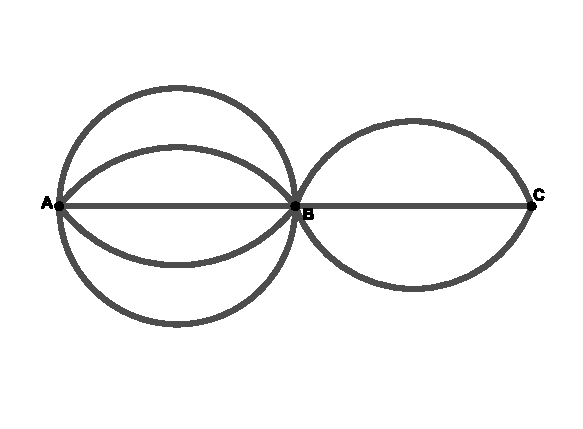
\includegraphics[width=0.6\textwidth]{Combinatoria/imgs/CAMINOSAaC.eps}
	\caption{Ejemplo \ref{EjemplociudadAaC}}
	\label{caminosAaC}
\end{figure}

\textit{Solución. }En este caso trataremos de contar de una forma distinta. Es útil nombrar los caminos como sigue

\begin{figure}[H]
	\centering
	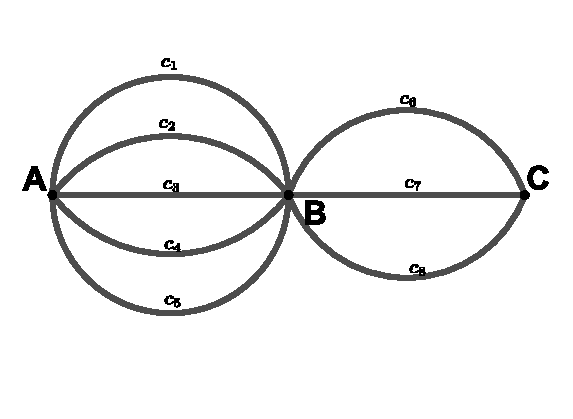
\includegraphics[width=0.6\textwidth]{Combinatoria/imgs/CAMINOSAaCrotulados.eps}
	\caption{Ejemplo \ref{EjemplociudadAaC} con caminos nombrados}
	\label{caminosAaCrotulados}
\end{figure}

En la siguiente tabla encontramos en la parte superior de la tabla están los caminos de la ciudad A a B, y en la parte vertical de la tabla los caminos posibles de B a C.


\begin{center}
	\begin{table}[H]
		\centering
		\begin{tabular}{|c|c|c|c|c|c|}
			\hline
			& $c_1$        & $c_2$        & $c_3$        & $c_4$        & $c_5$        \\ \hline
			$c_6$ & $c_1$ y $c_6$ & $c_2$ y $c_6$ & $c_3$ y $c_6$ & $c_4$ y $c_6$ & $c_5$ y $c_6$ \\ \hline
			$c_7$ & $c_1$ y $c_7$ & $c_2$ y $c_7$ & $c_3$ y $c_7$ & $c_4$ y $c_7$ & $c_5$ y $c_7$ \\ \hline
			$c_8$ & $c_1$ y $c_8$ & $c_2$ y $c_8$ & $c_3$ y $c_8$ & $c_4$ y $c_8$ & $c_5$ y $c_8$ \\ \hline
		\end{tabular}
		\caption{Caminos posibles para ir de A a C.}
		\label{tablacaminosAaC}
	\end{table}
\end{center}


En la tabla se ve que hay 15 caminos para ir de A a B y cada uno de ellos es distinto.
\vspace{0.3cm}

No siempre es útil utilizar este tipo de tablas o diagramas de árbol. Es por eso que debemos ayudarnos de un método mas sencillo.

\begin{defi}
	Cuándo al tratar de contar casos nos enfrentamos ante varias decisiones, es cuando usamos lo que se conoce como \textbf{Principio de Multiplicación}. Y lo que este dice, es que simplemente se multiplicar la cantidad de decisiones una tras otra. Para así, hallar la cantidad de todas las posibles opciones.
\end{defi}

\begin{ejemplo}
	La bandera de abajo debe ser pintada con 3 colores de tal manera que los colores que estén adyacentes sean distintos. Los 4 colores a la derecha son los que pueden ser usados. ¿De cuántas maneras puede ser pintada la bandera? 
\end{ejemplo}
\vspace{2cm}

(***Bandera de 3 franjas como de Colombia***)

\vspace{2cm}

\textit{Solución.} En primer lugar, hay 4 formas de pintar la franja de arriba. Luego de pintada esta, hay 3 formas de pintar la de la mitad, pues este color debe ser distinto al de arriba. Y para la franja de abajo, se podría pensar que hay 2 opciones porque no puedo usar el color del medio, pero note que podría volver a usar el color de la franjsa de arriba. Así, que para la de abajo hay 3 opciones. Usando el \textit{Principio de Multiplicación} habrían $4\times 3\times 3=24$ formas de pintar la bandera.

\begin{problem}
	Marta va a ir a una fiesta y deberá vestirse con un sombrero, un vestido y unos tacones. Ella tiene 3 sombreros distintos, tiene un vestido rojo y otro negro, y además tiene dos tacones, unos altos y otros bajos. ¿De cuántas maneras se podrá vestir Marta?\\
	a) Hacer un diagrama de árbol.\\
	b) Luego usar el principio de multiplicación y comparar.
\end{problem}

\begin{problem}
	¿Cuántos hay cuyos dígitos son todos distintos?
	\label{problema3digitosdistintos}
\end{problem}

\begin{ejemplo}
	El código binario utiliza únicamente los dígitos 1 y 0 para formar números. Por ejemplo, el 1101001 es un número binario de 7 dígitos. ¿Cuántos números binarios hay tales que tengan con máximo 4 dígitos?
\end{ejemplo}

\textit{Solución.} De longitud uno hay 2 números, el 1 y el 0. De longitud dos hay $2\times 2 = 4$. De longitud tres hay $2\times 2\times 2=8$. Y de longitud cuatro hay $2\times 2\times 2\times 2=16$ números. Así que en total hay $2+4+8+16=30$ números binarios tales que tienen como máximo 4 dígitos.

\section*{Postura Combinatorica.}
\begin{itemize}
	\item En los ejemplos trabajados hasta ahora y en general, es importante tomar una postura siempre del lado del objeto problema. Por ejemplo, al colorear la bandera, ponerse en el lado de quien pinta la bandera y ver que decisiones tiene que ir tomando esta persona.
	\item Las etapas del problema deben ser identificadas, por ejemplo al colorear la bandera fue útil decidir primero pintar el exterior y así hasta el interior. O en el caso de los número binarios fue necesario primero ver los números de 1 dígito, luego los de 2, después los de 3 y por último los de 4 dígitos.
	\item Por último saber ver cuál es la decisión más importante y aquella que tenga mas condiciones, por ejemplo en el problema de los números de 3 dígitos es importante saber que el primero dígito no puede ser cero. Así que debemos empezar a contar los casos por la decisión de poner el primer número.
\end{itemize}

\begin{ejemplo}
	¿Cuántos números pares de tres dígitos se pueden formar de tal manera que todos los dígitos sean distintos?
\end{ejemplo}

\textit{Solución 1.} Poniéndonos en el lugar del número, sabemos que este debe terminar en 0,2,4,6,8. Pero también debemos tener en cuenta que el 0 no puede ir en la primera posición. Así que tenemos varias condiciones para nuestro problema y es útil atacarlo por partes. El primer caso es cuando colocamos el 0 en la última posición, pues ahora para el primer dígito solo tendría 9 opciones. Pero si no se coloca el 2,4,6 0 8 en la última posición, se tendrán 8 opciones para el primer dígito, pues no puede ser 0 ni tampoco el que ya fue usado en la última posición. Es decir, el problema cambió, pues si pensamos en \ref{problema3digitosdistintos} allí las decisiones no cambiaban, en cambio acá las decisiones cambian cuando coloco o no coloco el 0 de último. Por tanto debemos contar ambos casos por aparte. Para el primero habrían $9\times 8 \times 1=72$ formas, pues como dijimos hay 9 formas para poner el primer número, 8 formas para el segundo porque no podemos usar el de la primera posición y 1 manera para el último, pues este dijimos que iba a ser 0. En el segundo caso habrían $8\times 8\times 4= 256$, pues para la primera posición dijimos que pueden ir 8, para la segunda se pensaría que pueden ir 7 pero se debe tener en cuenta que ahora si se puede usar el 0, por eso habrían 8 opciones para el segundo lugar y por último habrían 4 opciones para el último puesto (2,4,6,8). Así ya contamos ambos casos y se tendría que la cantidad total sería $72+256=328$.

\textit{Solución 2.} Otra manera de atacar el problema podría ser contar muchos casos y luego restar los que no funcionan. Por ejemplo contar todos los números que terminan en 0,2,4,6 o 8 y restar cuáles de estos números empiezan en 0. Entonces, para contar todos los que terminan en 0,2,4,6 o 8 sabemos que habrían 5 opciones para la última posición (0,2,4,6,8), luego habrían 9 opciones para la primera posición (Pues no se puede repetir el que ya se puso de último) y para la posición del medio habrían 8. Es decir, habrían $9\times 8\times 5=360$ maneras de formar números de 3 dígitos que terminen en 0,2,4,6 o 8. Pero de estos, hay casos que no sirven y son los que empiezan en 0. Para la última posición habrían 4 opciones (2,4,6,8. Ya que el 0 va a ir en la primera), para la primera posición hay 1 opción (Pues va el 0) y para la segunda 8 opciones (pues ya se usaron dos números). Así que hay $1\times 8\times 4=32$ números pares de tres dígitos que empiezan en 0. Así que restando estos de los anteriores tendríamos $360-32=328$.

\begin{ejemplo}
	¿De cuántas formas pueden hacer una fila 6 personas distintas?
\end{ejemplo}
\textit{Solución.} $6\times5\times4\times3\times2\times1$.
\vspace{0.2cm}

\begin{defi}
	Para evitar escribir $6\times5\times4\times3\times2\times1$ se usa $6!$ y se lee "\textit{seis factorial}". Es decir $n\times (n-1) \times (n-2) \cdots \times 3 \times 2\times 1 = n!$ y se lee "n factorial".
\end{defi}

\subsection*{\centering Práctica.}
Hallar otra expresión para cada una de las siguientes:
\begin{enumerate}[label=(\alph*)]
	\item $\frac{10!}{6!}$
	\item $\frac{5!4!}{6!}$
	\item $10!+11!$
	\item $\frac{6!+7!}{2!3!4!}$
	\item $n!(n^2 + 3n+2)$
	\item $\frac{(2n)!-(2n-1)!}{(2n)!-(n-1)!}$
	\item $\frac{(2n)!}{1\times 2\times 3\cdots \times (2n-1)}$
\end{enumerate}

\newpage
\begin{center}
	\vspace{-1cm}
	\section{ Ejercicios: Principio de multiplicación}\label{ejercicios:combinatoria:contandoListasDeNumeros}
\end{center}	
\begin{enumerate}
	\item ¿Cuántos números pares de tres dígitos pueden ser formados utilizando el 2,3,4 y 5 con la condición de que solo se puede usar máximo una vez cada dígito? (Ejercicio 1 de \textit{Primera Capacitación, básico, 2018, Principio de multiplicidad}).
	\item 
	\begin{enumerate}
		\item ¿Cuántos números naturales de tres cifras se pueden formar con los dígitos 2, 3, 4, 5, 6, 7, 8?
		\item ¿Cuántos números naturales de tres cifras \textbf{diferentes} se pueden formar con los dígitos 2, 3, 4, 5, 6, 7, 8? (Ejercicio 2 de \textit{Primera Capacitación, básico, 2018, Principio de multiplicidad}).
	\end{enumerate}
	\item ¿Cuántas palabras de tres letras se pueden formar únicamente usando las siguientes dos letras:\textit{a} y \textit{b}? .
	\item ¿De cuántas maneras se pueden sentar 5 personas en cinco puestos numerados del 1 al 5?
	\item Se desea ubicar 5 niños y 6 niñas en una fila de modo que los niños ocupen los lugares pares. ¿De cuántas formas puede hacerse? (Ejercicio 9 de \textit{Primera Capacitación, básico, 2018, Principio de multiplicidad}).
	\item Juan, Carlos, Tomás, María y José van al cine y les fueron asignadas cinco sillas consecutivas. ¿De cuántas formas se pueden sentar, si Juan y María están uno al lado del otro y nadie, además de María, está junto a Juan? (Ejercicio 10 de \textit{Primera Capacitación, básico, 2018, Principio de multiplicidad}).
	\item \label{problema_camino_flechas} De cuántas formas se puede ir del punto $A$ a $B$? (Ver figura \ref{problema7principiomultiplicacion})
	
	\begin{figure}[b]
		\centering
		\includegraphics[width=0.7\linewidth]{Combinatoria/imgs/problema7Principiomultiplicacion}
		\caption{Ver problema \ref{problema_camino_flechas}}
		\label{problema7principiomultiplicacion}
	\end{figure}
	
	\item Las placas de los carros son formadas por 3 letras (En un abecedario de 27 letras) y 3 dígitos. ¿Cuántas placas se pueden formar en total?
	\item Un grupo de 4 estudiantes (Alejandro, Blanca, Carlos, Daniela) quieren elegir el presidente y vicepresidente del salón. (Tomado de \cite{Contagem_e_probabilidade})
	\begin{enumerate}
		\item Haga una lista de todas las posibles formas de elegir al presidente(a) y vicepresidente(a). 
		\item ¿Cómo utilizaría el Principio de Multiplicación para contar?
	\end{enumerate} 
	\item \textbf{... ten cuidado.} \label{Problema_bandera_6colores} De cuántas formas se puede pintar la bandera (de la figura \ref{bandera6coloresprincipiomultiplicacion}) usando los seis colores de modo que las secciones adyacentes estén pintadas de diferente color?
	
	\begin{figure}
		\centering
		\includegraphics[width=0.7\linewidth]{Combinatoria/imgs/bandera_6_colores_Principiomultiplicacion}
		\caption{Ver Problema \ref{Problema_bandera_6colores}.}
		\label{bandera6coloresprincipiomultiplicacion}
	\end{figure}
	\item \textbf{... ten cuidado.} Se tiene un circulo dividido en 4 partes iguales. Martín tiene 5 colores en su mano y quiere saber de cuántas formas puede colorear el circulo con la condición de que las partes del circulo que comparten un lado no queden con el mismo color. (\textit{Cap 1, ejercicio 7 de }\cite{Contagem_e_probabilidade})
	\item Un examen consta de 8 preguntas, cada una de ellas con 5 respuestas múltiples (A,B,C,D y E). 
	\begin{enumerate}
		\item ¿Cuántos resultados distintos puede tener el examen?
		\item ¿En cuántos de estos resultados aparece solo una pregunta respondida con la letra A?
		\item ¿En cuántos de los resultados \textbf{no} aparece ninguna pregunta respondida con la letra A?
	\end{enumerate}
	\item \label{subconjuntos1,2,3}Dado el conjunto $\{ 1,2,3 \}$.
	\begin{enumerate}
		\item Haga una lista con todos los subconjuntos.
		\item ¿Cuántos subconjuntos hay?
	\end{enumerate}
	\item ¿Cuántos subconjuntos tiene el conjunto $\{1,2,3,\ldots ,n \}$? (Ver \ref{subconjuntos1,2,3})
	\item (\textit{Cap 1, ejercicio 13 de }\cite{Contagem_e_probabilidade})
	\begin{enumerate}
		\item ¿De cuántas maneras se puede formar una palabra de 6 letras (El abecedario tiene 27 letras) si la letra A debe ir en la palabra pero no puede estar en el primer lugar?
		\item ¿Y si la palabra no puede tener letras repetidas?
	\end{enumerate}
	\item Se escriben los números enteros del1 hasta el 2222. (\textit{Cap 1, ejercicio 16 de }\cite{Contagem_e_probabilidade})
	\begin{enumerate}
		\item Cuántas veces está escrito el dígito 0?
		\item En cúantos números aparece el dígito 0? 
	\end{enumerate}
	\item Cuántos enteros positivos de 4 dígitos hay en los cuales aparece el dígito 5? (\textit{Cap 1, ejercicio 17 de }\cite{Contagem_e_probabilidade})
	\item \textit{Teniendo 4 colores disponibles, de cúantas maneras se puede pintar una bandera de tres franjas si las franjas adyacentes deben ser de distinto color?}. Un estudiante da la siguiente solución: "Primero, voy a pintar las franjas extremas; para cada una, tengo 4 posibilidades de escoger. Después, yo pinto la franja central; como tiene que tener color diferente a sus dos franjas distintas, yo puedo escoger su color de apenas 2 formas. Luego, el número total de formas de pintar la bandera es $4\times 4\times 2=32$". La solución es corecta? Si no es correcta, dónde está el error? (\textit{Cap 1, ejercicio 19 de }\cite{Contagem_e_probabilidade}) 
	
	\item Hay 8 competidores en una final de 100 metros planos en una Olimpiada deportiva. La medalla de oro es para el primer puesto, la de plata para el segundo puesto y la de bronce para el tercer puesto. De cuántas formas pueden ser entregadas las medallas?. (1.4.7 de  \cite{ICP_Aops}) 
	
	\item (1.5.3 de  \cite{ICP_Aops}). 12 bolas numeradas del 1 al 12 son puestas en una urna. De cuántas maneras se pueden sacar 3 bolas, en orden, de la urna, si:
	\begin{enumerate}
		\item Cada bola se queda afuera una vez es sacada?
		\item Cada bola se devuelve a la urna después de ser sacada?
		\item La primera bola se devuelve a la urna  luego de ser sacada y la segunda se deja afuera una vez es sacada?
	\end{enumerate}
	
	\item Se desea ubicar 5 niños y 6 niñas en una fila de modo que los niños ocupen los lugares pares. ¿De cuántas maneras puede hacerse?. (Ejercicio 9 de \textit{Primera Capacitación, básico, 2018, Principio de multiplicidad}).
	
	\item Cuántos números de tres dígitos tienen exactamente un 0?. (Capítulo 2.4 Problema 2.8 de \cite{ICP_Aops}).
	
	\item Cuántos números de 3 dígitos tienen la propiedad de que el primer digito es al menos dos veces el segundo?. (2.4.2 de  \cite{ICP_Aops}).
	
	\item Cuántos números de 4 dígitos tienen la propiedad de que el ultimo digito es la suma de los primeros dos dígitos?. (2.4.3 de  \cite{ICP_Aops}).
	
	\item 	Cuántas secuencias de seis dígitos $x_1,x_2,…,x_6$ se pueden formar, dada la condicon de que los $x_i$ adyacentes no tienen la misma paridad? (paridad es ser par o impar, entonces por ejemplo $x_2$ y $x_3$ no pueden ser uno par y otro impar). (2.4.4 de  \cite{ICP_Aops}).
	
	\item Cuantas palabras de 3 letras se puede formar con las letras $A,B,C,D$ si se pueden repetir letras y se debe usar la letras A por lo menos una vez?. (2.2.1 de  \cite{ICP_Aops}).
	
	\item 
	\begin{enumerate}
		\item ¿De cuántas maneras se puede formar una palabra de 6 letras (Abecedario español de 27 letras) si la letra “A” debe ir en la palabra pero no en el primer lugar?
		\item ¿Y de cuántas maneras se puede formar si la palabra no puede tener letras repetidas?
	\end{enumerate}
	
	\item Suponga que tiene 6 camisas y 5 corbatas. De cuántas formas puede vestirse si debe usar camisa y corbata?. (1.4.1 de  \cite{ICP_Aops}).
	
	\item Para cada uno de ocho colores, tengo una camiseta y una corbata de ese color. De cuántas formas me puedo vestir si no quiero usar camisa y corbata del mismo color?. (1.4.2 de  \cite{ICP_Aops}).
	
	\item Cuántas placas de carro se pueden hacer si deben ser de dos letras seguidas de tres números?. (1.4.3 de  \cite{ICP_Aops}). 
	
	\item \label{problema_ciudadA_ciudadH} De cuantas formas se puede llegar de la ciudad A a la ciudad H siguiendo las direcciones de las flechas? (Ver figura \ref{ciudadaciudadh}). (2.2.3 de  \cite{ICP_Aops}). 
	
	\begin{figure}
		\centering
		\includegraphics[width=0.5\linewidth]{Combinatoria/imgs/ciudadA_ciudadH}
		\caption{ Problema \ref{problema_ciudadA_ciudadH}. }
		\label{ciudadaciudadh}
	\end{figure}
	
	\item Yo tengo dos sombreros. En uno hay bolas numeradas del 1 al 15 y en el otro hay bolas numeradas del 16 al 25. Yo primero elijo un sombrero, luego, de ese sombrero elijo 3 bolas, sin devolver las bolas una vez son sacadas. Cuántas diferentes formas de seleccionar las balotas son posibles?. (2.2.2 de  \cite{ICP_Aops}). 
	
	\item Cuántas placas de carro se pueden hacer si deben ser de tres letras seguidas de dos números pares y luego 2 números impares?. (1.4.4 de \cite{ICP_Aops}).
	
	\item Cuántos números de 5 dígitos tienen al menos un 0 (un dígito cero)?. (2.3.2 de \cite{ICP_Aops}).
	
	\item Tengo 6 camisetas, 6 pantalones y 6 sombreros. Cada uno de ellos viene en los mismos colores (Es decir, dado un color hay un sombrero un pantalón y un sombrero de ese color). Si no me quiero vestir con las 3 prendas del mismo color . De cuántas formas diferentes me puedo vestir?. (2.2.3 de \cite{ICP_Aops}).
	
	\item De cuántas formas se pueden sentar 7 personas en una fila de sillas si dos de ellos, William y Cata no se quieren sentar juntos?. (2.3.4 de \cite{ICP_Aops}).
	
	\item De cuántas maneras se pueden organizar cinco libros en una biblioteca?. (1.4.5 de \cite{ICP_Aops}).
	
	\item Suponga que se tienen 6 libros diferentes, de los cuales dos son de matemáticas. De cuántas maneras se pueden organizar los seis libros en una repisa si se quiere que los libros de matemáticas queden cada uno en un extremo?. (1.4.6 de \cite{ICP_Aops}).
	
	\item Cuántos números de 3 dígitos no son múltiplos de 7?. (Capítulo 2.3 Problema 2.6 de \cite{ICP_Aops}).
	
	\item Hay 8 estudiantes en la final de las Olimpiadas Matemáticas. De cuántas formas puede quedar el podio si este consiste de un primer puesto, un segundo puesto y un tercer puesto?.
	
	\item De cuántas formas puedo arreglar 3 libros de matemáticas y 5 de historia en una biblioteca si necesito que haya un libro de matemáticas al inicio y al final?. (Capítulo 2.5 Problema 2.11 de \cite{ICP_Aops}).
	
	\item En una granja hay 4 gallinas, 2 perros y 5 gatos, de cuantas formas se pueden colocar los animales en una casa de mascota si los animales de la misma especie deben quedar adyacentes?. (2.5.2 de \cite{ICP_Aops}).
	
	\item La familia Ordoñez tiene 5 niños, 3 niñas y 2 de las niñas son gemelas. De cuántas formas se pueden sentar en una fila de 8 sillas si las gemelas insisten en quedar juntas y la otra hermana no quiere sentarse al lado de ninguna de ellas?. (2.5.3 de \cite{ICP_Aops}).
	
	\item (1.4.5 de \cite{ICP_Aops}). Simplificar las siguientes expresiones sin usar calculadora: 
	\begin{enumerate}
		\item $\frac{9!}{8!}$.
		\item $\frac{42!}{40!}$.
		\item $8!-7!$.
	\end{enumerate}
	
	\item En Bucaramanga juega una lotería que consiste de 25 balotas numeradas del 1 al 25. Las balotas se introducen en una urna. Cuatro balotas son sacadas una a la vez y sus números son registrados. El número ganador se compone de los cuatro números extraídos, en el orden que fueron sacados. Cuántos números ganadores pueden haber, si:
	\begin{enumerate}
		\item Cada balota una vez es retirada de la urna no se vuelve a ingresar.
		\item b)	Cada balota se vuelve a meter en la urna una vez es extraída y registrada, para así poder sacar la siguiente balota.
	\end{enumerate}
	
	\item \label{problema_triangulos_piramide_contar} (2.2.4 de \cite{ICP_Aops}). Cuántos triángulos aparecen en el diagrama \ref{trainguloscontar}.
	\begin{figure}
		\centering
		\includegraphics[width=0.5\linewidth]{Combinatoria/imgs/traingulos_contar}
		\caption{Problema \ref{problema_triangulos_piramide_contar}.}
		\label{trainguloscontar}
	\end{figure}
	
	\item \label{problema_circulo_seiscolores} Con seis colores se quiere pintar la bandera (Figura \ref{circulo4franjas}) de manera que no queden espacios adyacentes del mismo color. De cuántas maneras se puede pintar?
	\begin{figure}
		\centering
		\includegraphics[width=0.4\linewidth]{Combinatoria/imgs/circulo_4_franjas}
		\caption{Problema \ref{problema_circulo_seiscolores}.}
		\label{circulo4franjas}
	\end{figure}
	
	\item Cuántas palabras de 3 letras pueden formarse si la segunda letra debe ser una vocal y la tercera letra debe ser distinta de la primera?.
	
	\item 40.	De cuántas formas es posible colocar 8 personas en una fila de modo que Camila y José no queden juntas y Marta y Martin si queden juntos?.
	
	\item 	Cuál es el máximo común divisor de 5!,10! Y 15!?. (1.33 de \cite{ICP_Aops}).
	
	\item De cuántas formas podemos colocar dos torres de ajedrez en el tablero de manera que ninguna amenace a la otra? (O sea que no estén en la misma fila ni en la misma columna).
	
	\item \textbf{Wow}. Cuántos enteros positivos menores que 500 se pueden expresar como la suma de dos cubos perfectos?.
	
	\item Juan, Carlos, Tomás, María y Jose van al cine y les fueron asignadas cinco sillas consecutivas. ¿De cuántas formas se pueden sentar, si Juan y María están uno al lado del otro y nadie, además de María, está junto a Juan?.
	
	\item Cuántos de los factoriales desde 1! Hasta 100! Son divisibles por 9?.
	
	\item Cuántos números naturales de 7 dígitos hay tales que tienen el dígito 4 exactamente tres veces y al dígito 8 exactamente dos veces?.
	
	\item Un candado de seguridad para una bicicleta necesita una clave de 5 dígitos. De cuántas formas se puede escoger la clave si debe ser un número impar, el dígito de la mitad debe ser par, el primer dígito debe ser múltiplo de 3, el segundo dígito debe ser un número primo? (Problema 2 \textit{UIS reto semanal bachillerato 2019}).
	
	\item \textbf{WOW}. Puede simplificar $P(n,k)P({n-k},j)$ donde $n,k$ y $j$ son enteros tales que $k\leq n$ y $j\leq {n-k}$?. (1.5.4 de \cite{ICP_Aops}).
	
	\item \textbf{WOW}. Cuál es el digito de las unidades de la suma $1!+2!+3!+\cdots+1000!?$. (1.35 de \cite{ICP_Aops}).
	
	\item \textbf{WOW}. De cuantas maneras se pueden elegir tres números del grupo de números 1,2,3,…100 de tal forma que el número más grande sea mayor que el producto de los otros dos? (el orden en que son sacados los números no importa). (2.4.5 de \cite{ICP_Aops}).
	
	\item Cuántos números de 4 dígitos tienen únicamente dígitos impares?. (2.16 de \cite{ICP_Aops}).
	
	\item Cuántas palabras de 3 letras pueden formarse con el alfabeto usual de 27 letras, si la primera letra debe ser una vocal?. (2.17 de \cite{ICP_Aops}).
	
	\item Cuántas claves de seguridad distintas se pueden formar con los dígitos del 1 al 5 si el segundo digito no puede ser el mismo que el primero y el tercero no puede ser el mismo que el segundo?. (2.18 de \cite{ICP_Aops}).
	
	\item Cuántas triplas (a,b,c) de números pares enteros positivos satisfacen $a^3+b^2+c\leq 50$?. (2.19 de \cite{ICP_Aops}).
	
	\item Cuántos números entre 100 y 200 no son cuadrados perfectos?. (2.20 de \cite{ICP_Aops}).
	
	\item Cuántos números de tres dígtios hay tales que el primer dígito es el triple que el tercer dígito?. (2.21 de \cite{ICP_Aops}).
	
	\item De cuantas formas se pueden sentar 6 niñas y 2 niños en una fila si los 2 niños insisten en sentarse juntos?. (2.22 de \cite{ICP_Aops}).
	
	\item Cuantos números de 4 dígitos tienen el segundo digito par y el cuarto digito al menos dos veces mayor que el segundo?. (2.23 de \cite{ICP_Aops}).
	
	\item Cuántos números de 3 digitos existen tales que la suma del digito de las centenas y el de las decenas es igual al de las unidades?. (2.26 de \cite{ICP_Aops}).
	
	\item La suma digital de un número es la suma de sus dígitos. Para cuantos números entre 24 y 125 incluyéndolos la suma digital es múltiplo de 7?. (2.27 de \cite{ICP_Aops}).
	
	\item \textbf{WOW.} Los $n$ miembros de un comité son numerados desde 1 hasta $n.$ Uno de los miembros es designado como el “cansón”. Los $n$ miembros se sientan en una fila de $n$ sillas, pero ningún miembro con un número mayor al del “cansón” se puede sentar inmediatamente a la derecha del “cansón”. Suponga que el “cansón” es el miembro $p$ con $1\leq p\leq n$. Encuentre una formula, en términos de $n$ y $p$, para el número de formas que se pueden sentar los miembros del comité. (2.29 de \cite{ICP_Aops}).
	
	\item \label{problema_tablaNOON} \textbf{WOW.} De cuántas formas usted puede deletrar la palabra NOON con la tabla \ref{tabla_NOON}? Usted puede empezar con cualquier letra, luego en cada paso usted se puede mover arriba, abajo, a la derecha, a la izquierda o en diagonal hasta que termine de deletrar la palabra. Usted no puede pasar por la misma casilla dos veces. (2.30 de \cite{ICP_Aops}).
	
	\begin{table}[]
		\centering
		\begin{tabular}{|l|l|l|l|}
			\hline
			N & N & N & N \\ \hline
			N & O & O & N \\ \hline
			N & O & O & N \\ \hline
			N & N & N & N \\ \hline
		\end{tabular}
		\caption{Problema \ref{problema_tablaNOON}.}
		\label{tabla_NOON}
	\end{table}
	
	\item Un número palíndromo es un número que se lee igual de derecha a izquierda que de izquierda a derecha, por ejemplo 12321. (2.31 de \cite{ICP_Aops}).
	\begin{enumerate}
		\item Cuántos números palíndromos hay de 4 digitos?
		\item Cuántos números palíndromos hay de 5 digitos?
		\item \textbf{Wow} Cuántos números palíndromos hay de $n$ digitos?
		\item \textbf{Woww}. Suponga que hacemos una lista con los números palíndromos de k dígitos que están formados únicamente con los dígitos 8 y 9, y además tiene al menos un 8 y al menos un 9. Cuál es el valor más pequeño de k tal que hayan al menos 2019 números en la lista? 
	\end{enumerate}
	
	\item Sea $S$ un cubo. Calcule cuantos planos pasan a través de al menos 3 vértices de $S$. (2.32 de \cite{ICP_Aops}).
	
	\item \textbf{Woww}. Cuantos ceros se escriben al escribir todos los enteros desde 1 hasta 256 en binario?. (2.33 de \cite{ICP_Aops}).
	
	\item Cuántas palabras de 5 letras (donde cualquier lista de 5 letras se considera una palabra) tienen al menos dos letras iguales consecutivas?. (2.34 de \cite{ICP_Aops}).
	
	\item Un número entero positivo es llamado \textit{"estable"} si al menos uno de sus dígitos tiene el mismo valor que su posición en el número. Por ejemplo, $78247$ es estable debido a que un 4 aparece en la 4ta posición. Cuántos números estables de tres dígitos hay?. (Ejercicio 26 de \textit{XXIX Competencia Regional de Matemáticas,Nivel Intermedio UAN 2019}). 
\end{enumerate}
\newpage


\chapter{Principio de Inclusión y Exclusión}\label{Pinclusionyexclusion}
\vspace{3cm}

(***importante aclarar conjuntos....la diferencia entre ``y" y la ``o".)
\vspace{3cm}




\newpage
\begin{center}
	\vspace{-1cm}
	\section{ Ejercicios: Principio de Inclusión y Exclusión}
\end{center}	
\begin{enumerate}
	\item En un colegio hay 170 estudiantes. Algunos de ellos asisten a la lúdica de Club matemático,  cine o fútbol, que se realizan por las tardes. Se sabe que
	\begin{itemize}
		\item 65 estudiantes asisten a Club matemático.
		\item 96 asisten a cine.
		\item 94 asisten a fútbol.
		\item 35 estudiantes asisten únicamente a la lúdica de cine.
		\item 42 asisten a cine y fútbol.
		\item 40 asisten a Club matemático y fútbol.
		\item 22 estudiantes asisten a las tres lúdicas.
	\end{itemize}
	Con base en la información anterior,
	\begin{enumerate}
		\item ¿Cuántos estudiantes están únicamente en el Club matemático?
		\item ¿Cuántos están únicamente en cine?
		\item ¿Cuántos de ellos asisten a cine o fútbol?
		\item ¿Cuántos asisten por lo menos a una de las lúdicas?
		\item ¿Cuántos estudiantes no asisten a ninguna lúdica?
	\end{enumerate}
\end{enumerate}
\newpage

	
	%\input{Combinatoria/Principio_de_multiplicacion/cap_principio_multiplicacion.tex}	
	%\input{Combinatoria/inclusion_y_exclusion/cap_inclusion_exclusion.tex}
	
	
	\part{Geometr\'ia}
	\chapter{Introducción}
\label{seccion_geometria_introduccion}

\section{Puntos, segmentos, marcas de igualdad.}\label{subseccion_puntos_segmentos_etc}
\textit{Que es un Punto?} La mínima marca que deja un lápiz, un pobre solo en la nada.

\begin{figure}[H]
	\centering
	\includegraphics[width=0.15\linewidth]{Geometria/imgs/punto.png}
%	\caption{}
	\label{punto}
\end{figure}
\textbf{OJO.} Lo debemos nombrar usando \textbf{letras mayúsculas}.

\begin{figure}[H]
	\centering
	\includegraphics[width=0.15\linewidth]{Geometria/imgs/puntos}
	%	\caption{}
	\label{puntos}
\end{figure}

\textit{Ahora si tenemos dos puntos, cómo hacemos para llegar de uno al otro?}

\begin{figure}[H]
	\centering
	\includegraphics[width=0.4\linewidth]{Geometria/imgs/puntos_A_y_B}
	%	\caption{}
	\label{puntos_A_y_B}
\end{figure}

\textbf{Rta:} Podriamos con muchos caminos, \textit{como cuales?}. De estos \textit{cuál es el más corto?} \textbf{Rta:} El \textbf{segmento}.

\begin{figure}[H]
	\centering
	\includegraphics[width=0.5\linewidth]{Geometria/imgs/segmento_AB}
	\caption{Segmento $\overline{AB}$}
	\label{segmento_AB}
\end{figure}

\textbf{OJO.} Un \textbf{segmento} se denota por sus puntos extremos, en este caso el de la figura \ref{segmento_AB} se denota como \textbf{segmento $\overline{AB}$ }. A veces para referirnos a la longitud simplemente decimos $AB=12cm$. 


\rule{\textwidth}{0.1mm}
\begin{act}
	Construir en geogebra un lado $AB$ y luego construir otro lado $CD$ que sea el triple que este (Mejor si logra crear un deslizador para el valor de la razón incluso si logra crear un deslizador).
\end{act}
\rule{\textwidth}{0.1mm}

\textit{Cúantos puntos tiene un segmento? } \textbf{Rta:} Infinitos.

\begin{figure}[H]
	\centering
	\includegraphics[width=0.4\linewidth]{Geometria/imgs/punto_C_sobre_AB}
	\caption{Un punto $C$ sobre $\overline{AB}$}
	\label{punto_C_sobre_AB}
\end{figure}

\begin{figure}[H]
	\centering
	\includegraphics[width=0.4\linewidth]{Geometria/imgs/puntos_C_D_sobre_AB}
	\caption{Dos puntos, $C$ y $D$ sobre $\overline{AB}$}
	\label{puntos_C_D_sobre_AB}
\end{figure}

\textit{Entre un par de puntos en un segmento siempre encontrará otro punto?} \textbf{Rta:} Si.

\rule{\textwidth}{0.1mm}
\begin{act}
	Construir en geogebra un segmento $\overline{AB}$ e ir poniendo puntos y haciendo zoom para ver que siempre entre cada par de puntos habrá otro.
\end{act}
\rule{\textwidth}{0.1mm}

\textbf{OJO.} Leer lo siguiente a ver que se entiende, es un ejercicio útil a la hora de resolver problemas, identificar palabra por palabra.\\
\textit{Cuántos puntos \textbf{equidistantes} a $A$ y $B$ hay en un segmento $\overline{AB}$?} \textbf{Rta:} Es decir punto $X$ tal que $AX=XB$, hay uno ver figura \ref{punto_medio}.
 
\begin{figure}[H]
	\centering
	\includegraphics[width=0.5\linewidth]{Geometria/imgs/punto_medio}
	\caption{Punto medio  $X$ de $\overline{AB}$, es decir, $AX=XB$}
	\label{punto_medio}
\end{figure}

Para denotar longitudes iguales se usan marcas, ejemplos:

\begin{figure}[H]
	\centering
	\includegraphics[width=0.5\linewidth]{Geometria/imgs/notacion_longitud_igual}
	\caption{$AX=XB$}
	\label{notacion_longitud_igual}
\end{figure}

\begin{figure}[H]
	\centering
	\includegraphics[width=0.5\linewidth]{Geometria/imgs/notacion_en_un_triangulo}
	\label{notacion_en_un_triangulo}
\end{figure}


\begin{exer}{\ \\}
		Si no fuera sobre el segmento, habrán mas puntos equidistantes a $A$ y $B$?
\end{exer}

\newpage
\begin{center}
		\vspace{-1cm}
		\subsection{ Puntos, segmentos, marcas de igualdad.}\label{ejercicios_puntos_segmentos_etc} 
\end{center}
			
\begin{enumerate} 
	\item  En la figura \ref{notacion_longitud_igual} se tiene que $AB=10cm$, entonces cuánto mide $AX$?
	\item\label{ejer_problema_segmento_dividido_en_tres} En la figura \ref{problema_segmento_dividido_en_tres} se tiene que $HK=12cm$, entonces cuánto mide $IJ$?
		
		\begin{figure}[H]
			\centering
			\includegraphics[width=0.8\linewidth]{Geometria/imgs/problema_segmento_dividido_en_tres}
			\caption{Ejercicio \ref{ejer_problema_segmento_dividido_en_tres}.}
			\label{problema_segmento_dividido_en_tres}
		\end{figure}
	\item \label{ejer_problema_2} En la figura \ref{problema_2} se tiene que $AB=12cm$, si $AX = XB$ y $AL=LX$ entonces cuánto mide $LB$?
		
		\begin{figure}[H]
			\centering
			\includegraphics[width=0.8\linewidth]{Geometria/imgs/problema_2}
			\caption{Ejercicio \ref{ejer_problema_2}.}
			\label{problema_2}
		\end{figure}
	
	\item \label{ejer_problema_3} En la figura \ref{problema_3} se tiene que $NO=12cm$, si $OB=4cm$ y $AX=3cm$ entonces cuánto es el perimetro de $NOBA$?
	
	\begin{figure}[H]
		\centering
		\includegraphics[width=0.6\linewidth]{Geometria/imgs/problema_3}
		\caption{Ejercicio \ref{ejer_problema_3}.}
		\label{problema_3}
	\end{figure}		
\end{enumerate}
\newpage

\section{Rectas, rayo, paralelas, rectas concurrentes}\label{subseccion_rayo_recta_paralelas_etc}

Sabiamos que con un segmento podíamos ir de un punto a otro, ahora seguiremos derecho al pasar por un punto hasta donde queramos mediante el \textbf{rayo}.

\begin{figure}[H]
	\centering
	\includegraphics[width=0.8\linewidth]{Geometria/imgs/rayo}
	\caption{Un \textbf{rayo} $\overset\rightarrow{PQ}$ que parte de $P$ y pasa por $Q$.}
	\label{rayo}
\end{figure}

\textbf{OJO. } Al \textbf{rayo} que parte de $P$ y pasa por $Q$ se le denota como $\overrightarrow{PQ}$.\\

\textit{Será que $\overrightarrow{PQ}$ es lo mismo que $\overrightarrow{QP}$?} \textbf{Rta:} No.\\
\textit{Coloquen un punto que esté en  $\overrightarrow{PQ}$ y no esté en  $\overrightarrow{QP}$ }\\
\textit{Coloquen un punto que esté en  $\overrightarrow{PQ}$ y en  $\overrightarrow{QP}$ }\\
\textit{Coloquen un punto que esté en  $\overrightarrow{QP}$ y no esté en  $\overrightarrow{PQ}$ }.\\

Si ahora seguimos derecho al pasar por ambos puntos hasta donde queramos obtenemos una \textbf{recta}.
\begin{figure}[H]
	\centering
	\includegraphics[width=0.8\linewidth]{Geometria/imgs/recta}
	\caption{Una \textbf{recta} $\overset\leftrightarrow{RS}$ o $l$ que pasa por $R$ y $S$.}
	\label{recta}
\end{figure}

\textbf{OJO. } A la \textbf{recta} que que pasa por $R$ y $S$ se le denota como $\overleftrightarrow{RS}$ o se le llama con una letra minúscula ejemplo: $l$.\\

\textit{Si se trazan dos rectas en cuántos puntos se pueden cortar?} \textbf{Rta: }Puede ser en 0 punto como en la figura \ref{paralelas}

\begin{figure}[H]
	\centering
	\includegraphics[width=0.7\linewidth]{Geometria/imgs/paralelas}
	\caption{Las rectas $k$ y $l$ son paralelas o sea $l||k$.}
	\label{paralelas}
\end{figure}

\textbf{OJO. }Un par de rectas $k$ y $l$ son \textbf{paralelas} si nunca se cortan, esto se denota como $l||k$ .\\

\textbf{Rta: }Puede ser en 1 punto como en la figura \ref{concurrentes}

\begin{figure}[H]
	\centering
	\includegraphics[width=0.85\linewidth]{Geometria/imgs/concurrentes}
	\caption{Las rectas $n$ y $b$ son concurrentes o se intersectan en $S$.}
	\label{concurrentes}
\end{figure}

\textbf{OJO. }Un par de rectas $n$ y $n$ son \textbf{concurrentes} o se \textbf{intersectan} si comparten 1 punto.\\

\textit{Será que dos rectas se pueden intersectar en 2 puntos ?}

\textbf{OJO.} Si varios puntos están sobre una misma recta se dice que son \textbf{colineales}, ver figura \ref{colineales}.

\begin{figure}[H]
	\centering
	\includegraphics[width=0.85\linewidth]{Geometria/imgs/colineales}
	\caption{Los puntos $U$, $S$ y $V$ son colineales pues están todos sobre la recta $b$.}
	\label{colineales}
\end{figure}

\textit{Es diferente la recta $\overleftrightarrow{US}$ que $\overleftrightarrow{VS}$ ?}\\

\newpage
\begin{center}
	\vspace{-1cm}
	\subsection{Ejercicios: Rectas, rayo, paralelas, rectas concurrentes.}\label{ejercicios_subseccion_rayo_recta_paralelas_etc}
\end{center}
	\begin{enumerate}
		\item Realizar los puntos del 1. al 9.
		\begin{figure}[H]
			\centering
			\includegraphics[width=\linewidth]{Geometria/imgs/Clemens_p14_1to9}
			%\caption{Los puntos $U$, $S$ y $V$ son colineales pues están todos sobre la recta $b$.}
			\label{Clemens_p14_1to9}
		\end{figure}
		\item Realizar los puntos del 12. al 14.
		\begin{figure}[H]
			\centering
			\includegraphics[width=\linewidth]{Geometria/imgs/CLEMENS_p15_12to14}
			%\caption{Los puntos $U$, $S$ y $V$ son colineales pues están todos sobre la recta $b$.}
			\label{CLEMENS_p15_12to14}
		\end{figure}
		\item (1.2.1 de \cite{Aops_Geometria}). Alicia está pensando en una recta. Cuántos puntos en esta recta le debe mostrar a Bernardo para que el sepa en que recta está pensando ella?
		\item (1.2.2 de \cite{Aops_Geometria}). $M$ es el punto medio de $\overline{AB}$ y $N$ es el punto medio de $\overline{BM}$. Si $BN=4cm$, cuánto mide $AB$?
		\item (1.2.3 de \cite{Aops_Geometria}). $P,Q,R,S$ y $T$ están en una recta $k$ tal que $Q$ es el punto medio de $\overline{PT}$, $R$ es el punto medio de $\overline{QT}$  y $S$ es el punto medio de $\overline{RT}$. Si $PS=9cm$, cuánto mide $PT$?
		\item (1.2.4 de \cite{Aops_Geometria}). \textbf{(Woww)}. Los puntos $A,B,C,D$ y $E$ están sobre el segmento que tiene como puntos finales a $A$ y $E$. Los puntos están en el orden que fueron mencionados de izquierda a derecha de forma que $CD=\frac{AB}{2}$, $BC=\frac{CD}{2}$, $AB=\frac{AE}{2}$ y $AE=12cm$. Cuánto mide $AD$?		
	\end{enumerate}
\newpage

\section{Circulo, radio, tangente, secante, cuerda, diámetro, arco}\label{subseccion_de_introduccion_geo_circulo}

\rule{\textwidth}{0.1mm}
\begin{act_clase} \textbf{En el circulo}\\ (\textit{Basado en \cite{Aops_Geometria} problemas 1.1 y 1.2}){\ \\}
	
	\textbf{Materiales:} 
	\begin{enumerate}
		\item Regla.
		\item Compás.
		\item Lápiz.
	\end{enumerate}

	\textbf{Desarrollo:}
	\begin{enumerate}
		\item Marcar un punto $O$, luego con el solo uso de la regla encontrar la mayor cantidad de puntos que estén a 2cm de $O$, nombrar estos puntos $A,B,C,D,\dots$ y así sucesivamente. Si se dibujan muchos de estos puntos que figura se forma?
		\vspace{6cm}
		
		\begin{itemize}
			\item Esto es un \textbf{circulo}, donde $O$ es el \textbf{centro del círculo}. En vez de decir \textit{``circulo con centro en $O$""} se puede decir: $\odot O$. 
			\item El segmento \textbf{$\overline{AB}$ es un radio} de $\odot O$. Mencione otros radios de $\odot O$: \vspace{1cm}
			
			\item La distancia del centro $O$ a los puntos también se conoce como radio, es decir \textbf{el radio del $\odot O$ es de 2cm} .
		\end{itemize}
		
		
		\item Dado $\odot X$ de radio $1.5cm$ trazar:
		\begin{enumerate}[label=\Alph*)]
				\item Una recta $l$ que corte al circulo en cero puntos. \vspace{5cm}
				\item Una recta $k$ que corte al circulo en 1 punto. \vspace{5cm}
						\begin{itemize}
							\item Esta recta que solo toca en 1 punto al circulo recibe el nombre de: \textbf{recta tangente}. Se dice entonces que $l$ es tangente a $\odot X$.
						\end{itemize}
				\item Una recta $m$ que corte al circulo en 2 puntos. \vspace{5cm}
						\begin{itemize}
							\item Esta recta que intersecta en 2 puntos al circulo recibe el nombre de: \textbf{recta secante}. Se dice entonces que $m$ es secante a $\odot X$.
						\end{itemize}
				\item Habrá una recta que corte en 3 puntos al circulo?
		\end{enumerate}
		\item Dibujar un $\odot O$ de radio $2cm$ y un recta $m$ que sea tangente a $\odot O$ en un punto $P$.\vspace{5cm}
		\item Dibujar un $\odot R$ de radio $1.7cm$ y un recta $s$ que sea secante a $\odot R$ en los puntos $P$ y $Q$. \vspace{5cm}
		
		\item Dado $\odot Y$ de radio $1.2cm$ trazar:
			\begin{enumerate}[label=\Alph*)]
				\item Todas las formas posibles en que un segmento $\overline{RS}$ corte al circulo en cero puntos. \vspace{5cm}
				\item Todas las formas posibles en que un segmento $\overline{PQ}$ corte al circulo en 1 punto. \vspace{5cm}
				\item Todas las formas posibles en que un segmento $\overline{CT}$ corte al circulo en 2 puntos. \vspace{5cm}
				\begin{itemize}
					\item En el caso en el los puntos del segmento están sobre el circulo es especial. Se dice en este caso que el segmento es una \textbf{cuerda}. 
				\end{itemize}
			\end{enumerate}
		\item Dibuje un $\odot M$ de radio $3cm$ y dibuje:
				\begin{enumerate}[label=\Alph*)]
						\item Una cuerda $\overline{AB}$ de forma que $AB=6cm$.
						\item Una cuerda $\overline{RS}$ de forma que $AB=4cm$.
						\item Una cuerda $\overline{PQ}$ de forma que $AB=2cm$.
				\end{enumerate}
		 		\vspace{8cm}
		 \item Qué diferencia hay entre una cuerda y una secante?\vspace{1.5cm}
		 \item Dado $\odot Q$ de radio cualquiera, construir una cuerda $\overline{XY}$ que pase por $Q$.\vspace{4cm}
			 \begin{enumerate}[label=\Alph*)]
			 		\item Es $Q$ equidistante a $X$ y $Y$? Por qué?\vspace{1.5cm}
			 \end{enumerate}
		 	\begin{itemize}
		 		\item La cuerda que pasa por el centro de un circulo recibe el nombre de \textbf{diámetro}. En el anterior ejemplo tenemos entonces que el diámetro es la cuerda $XY$. Habrán más diámetros? Dibuje mas puntos si es necesario y mencioe acá otros diámetros:\vspace{2cm}
		 		
		 	\end{itemize}
	 	\item Cuántos diámetros tiene un circulo?
	 	\item Trazar $\odot Q$ de forma que los diámetros del circulo midan $4cm$.\vspace{5cm}
	 	\item Trazar $\odot N$ de radio $1.5cm$ y dos puntos $A$ y $H$ sobre el circulo. Luego trazar la curva más corta que une a $A$ y $H$ sobre el circulo.\vspace{4cm}
	 	\begin{itemize}
	 		\item La curva que une a $A$ y $H$ es un \textbf{arco}. Es la curva mas corta que une dos puntos sobre el circulo.
	 	\end{itemize}
	\end{enumerate}
\end{act_clase}
\rule{\textwidth}{0.1mm}

\newpage
\begin{center}
	\vspace{-1cm}
	\subsection{Ejercicios: Circulo, radio, tangente, secante, cuerda, diámetro, arco}\label{ejercicios_subseccion_de_introduccion_geo_circulo}
\end{center}
	\begin{enumerate}				
			\item \label{p131_aops_geo} (1.3.1 de \cite{Aops_Geometria}). En la Figrua \ref{aops_geo_p_1_3_1} identifique cuando cada uno de los siguientes es una secante, una recta, una cuerda, un radio, un diámetro o una recta tangente a $\odot O$. (Si cumple con varios terminos, mencionelos todos):
			\begin{enumerate}[label=\Alph*)]
					\item $\overline{CO}$.
					\item $\overleftrightarrow{EF}$.
					\item $\overline{CD}$.
					\item $\overline{AB}$.
					\item $\overleftrightarrow{CD}$.
			\end{enumerate}
			
				\begin{figure}[H]
					\centering
					\includegraphics[width=0.35\linewidth]{Geometria/imgs/aops_geo_p_1_3_1}
					\caption{Ejercicio \ref{p131_aops_geo}}
					\label{aops_geo_p_1_3_1}
				\end{figure}
			\item \label{p132_aops_geo} (1.3.2 de \cite{Aops_Geometria}). Suponga que tiene un punto $P$ fuera de un circulo cualquiera. Siempre es posible trazar una recta que pase por $P$ y sea tangente al circulo?
			
			\item \label{p133_aops_geo} (1.3.3 de \cite{Aops_Geometria}). Cuánto es la máxima cantidad posible que puede haber de puntos de intersección entre un cirulo y un triángulo?
			
			\item \label{p134_aops_geo} (1.3.4 de \cite{Aops_Geometria}). \textbf{Wow}. Se tienen dos circulos y tres rectas sobre el mismo plano. Cuánto es la máxima cantidad posible que puede haber de puntos de intersección donde al menos dos figuras se intersectan?
	\end{enumerate}
\newpage

\section{Copiando segementos}\label{Copiando_segmentos}
\rule{\textwidth}{0.1mm}
\begin{act_clase} \textbf{Copiando segmentos} \\ (\textit{Basado en \cite{Aops_Geometria} problemas 1.3 y 1.4}){\ \\}
	\textbf{Materiales:} 
	\begin{itemize}
		\item Regla.
		\item Compás.
		\item Lápiz.
		\item Transportador.
	\end{itemize}
	
	\textbf{Desarrollo:} De acá en adelante no se puede usar la regla para medir!
	\begin{enumerate}
		\item Dados dos puntos $A$ y $B$ donde quieran, trazar un $\odot A$ que pase por $B$ y se llame $c_1$ y otro $\odot B$ que pase por $A$ y se llame $c_2$. \vspace{8cm}
		
		\begin{itemize}
				\item \textbf{Dato:} Al igual que las rectas, también podemos llamar a los circulos con letras minúsculas.
		\end{itemize}
	
		\item Trazar un segmento $\overline{AB}$ de longitud aleatoria, luego hacer un circulo $\odot M$ cuyo radio sea $\overline{AB}$
		\vspace{6cm}
		
		\item (1.3 de \cite{Aops_Geometria}). Usar el compás para hallar en la recta $k$ un punto $Y$ tal que $AB=XY$.
			\begin{figure}[H]
				\centering
				\includegraphics[width=0.8\linewidth]{Geometria/imgs/aops_geo_1_3}
				%\caption{}
				\label{aops_geo_1_3}
			\end{figure}

		\item \label{p1_4_aopsgeo}(1.4 de \cite{Aops_Geometria}). En la figura \ref{aops_geo_1_3} se muestran los segmentos $\overline{AB}$ y $\overline{MN}$. Con regla y compás construir:
			\begin{figure}[H]
				\centering
				\includegraphics[width=0.5\linewidth]{Geometria/imgs/aops_geo_1_4}
				\caption{Ejercicio \ref{p1_4_aopsgeo}}
				\label{aops_geo_1_4}
			\end{figure}
		\begin{enumerate}[label=\Alph*)]
				\item Un segmento de longitud $AB+MN$. \vspace{6cm}
				\item Un segmento de longitud $AB-MN$. \vspace{7cm}
				\item Un segmento de longitud $MN-AB$. \vspace{7cm}				
		\end{enumerate}

		\item \label{p1_4_1_aopsgeo} (1.4.1 de \cite{Aops_Geometria}). Con los segmentos de la figura \ref{aops_geo_1_4_1}, construir:
			\begin{figure}[H]
				\centering
				\includegraphics[width=0.3\linewidth]{Geometria/imgs/aops_geo_1_4_1}
				\caption{Ejercicio \ref{p1_4_1_aopsgeo}}
				\label{aops_geo_1_4_1}
			\end{figure}
			\begin{enumerate}[label=\Alph*)]
				\item Un segmento de longitud $AB+CD-EF$. \vspace{6cm}
				\item Un segmento de longitud $2AB$. \vspace{6cm}
				\item Un segmento de longitud $AB-2EF+3CD$. \vspace{5cm}				
			\end{enumerate}
		
	\end{enumerate}
\end{act_clase}
\rule{\textwidth}{0.1mm}
\newpage

\section{Ángulos}\label{subseccion_angulos_intro}

\subsection{Introducción, notacion, clasificacion, medicion.}\label{subsection_intro_notacion_clasificacion_medicion}

\begin{itemize}
	\item Cuando dos rayos comparten el origen forman un \textbf{ángulo}. Este vértice se llama \textbf{vértice del ángulo}. 
	\item Por ejemplo en le Figura \ref{Angulo_XOY} se presenta un ángulo formado por los rayos $\overrightarrow{OX}$ y $\overrightarrow{OY}$, el cuál se denota como $\angle XOY$, \textbf{se nombre el vértice en la mitad}, también se puede llamar $\angle YOX$ \textbf{Ojo:} Pero no $\angle YXO$ ni  $\angle XYO$.
	\item En este caso como solo está este ángulo también se puede denotar como $\angle O$.
\end{itemize}


\begin{figure}[H]
	\centering
	\includegraphics[width=0.3\linewidth]{Geometria/imgs/Angulo_XOY}
	%\caption{Ángulo $\angle XOY$, también puede ser llamado $\angle YOX$}
	\label{Angulo_XOY}
\end{figure}

\textit{Si $\overleftrightarrow{AB}$ y $\overleftrightarrow{CD}$ se intersectan en un punto $P$ como muestra la Figura \ref{dos_angulos}, es claro a cuál ángulo nos referimos si decimos simplemente $\angle P$?}


\begin{figure}[H]
	\centering
	\includegraphics[width=0.3\linewidth]{Geometria/imgs/dos_angulos}
	%\caption{No es correcto decir solo \(\angle P\)}.
	\label{dos_angulos}
\end{figure}

\textbf{Uso de transportador}. Saben usarlo?


\clearpage

%\rule{\textwidth}{0.1mm}

\begin{center}
	$\textbf{\textit{Actividad de clase}}$
\end{center}

\textit{Basado en \cite{Aops_Geometria} problemas 2.1 a 2.5}

\textbf{Materiales:} 
\begin{itemize}
	\item Regla.
	\item Lápiz.
	\item Transportador.
\end{itemize}

\textbf{Desarrollo:}
\begin{enumerate}
	\item Dibujar 3 ángulos abajo, luego intercambiar con otro compa?ero y medir los ángulos que el dibujó. Preguntale si mediste el ángulo que el dibujó.\vspace{6cm}
	\item Cuánto mide el ángulo mas grande que se puede dibujar? Dibujalo. \vspace{5cm}
	\item \label{p22_aops_geo} (2.2 de \cite{Aops_Geometria}). En la Figura \ref{P22_AOPS_GEO} se muestran cuatro ángulos. En cada caso, el punto $O$ es el centro del circulo. $\angle AOB$ corta $\frac{1}{4}$ del circulo,  $\angle COD$ corta $\frac{1}{3}$, $\angle EOF$ corta $\frac{1}{12}$ y $\angle GOH$ corta $\frac{1}{8}$.
	\begin{figure}[H]
		\centering
		\includegraphics[width=0.75\linewidth]{Geometria/imgs/P22_AOPS_GEO}
		\caption{Punto \ref{p22_aops_geo}}
		\label{P22_AOPS_GEO}
	\end{figure}
	
	\begin{enumerate}[label=\Alph*)]
		\item Cuántos grados mide el ángulo $\angle AOB$?
		\item Cuántos grados mide el ángulo $\angle COD$?
		\item Cuántos grados mide el ángulo $\angle EOF$?
		\item Cuántos grados mide el ángulo $\angle GOH$?		
	\end{enumerate}
	
	\item \label{p23_aops_geo} (2.3 de \cite{Aops_Geometria}). En la Figura \ref{P23_AOPS_GEO} se tiene que $\angle WOY=60\degree$ y $\angle WOX=20\degree$, cuánto mide $\angle XOY$?
	\begin{figure}[H]
		\centering
		\includegraphics[width=0.3\linewidth]{Geometria/imgs/P23_AOPS_GEO}
		\caption{Punto \ref{p23_aops_geo}.}
		\label{P23_AOPS_GEO}
	\end{figure}
	
	\item \label{P_suma_ang_1}En la Figura \ref{suma_ang_1} se tiene ahora que $\angle WOX=15\degree$ y $\angle XOY=55\degree$, cuánto mide $\angle WOY$?
	\begin{figure}[H]
		\centering
		\includegraphics[width=0.3\linewidth]{Geometria/imgs/P23_AOPS_GEO}
		\caption{Punto \ref{P_suma_ang_1}.}
		\label{suma_ang_1}
	\end{figure}
	
	\item \label{ej_8_1_medidaangulos} (Ejemplo 8.1 de \cite{Udea_geometria}) Si se tienen dos ángulos $\angle \alpha$ y $\angle \beta$ que miden $42\degree$ y $35\degree $ respectivamente, cuánto mide $\alpha + \beta$?
	
	
	\item \label{p24_aops_geo} (2.3 de \cite{Aops_Geometria}). Suponga que se mide un ángulo \textit{``interior"}. Como se ve en la figura \ref{P24_AOPS_GEO}, va a haber un ángulo \textit{``exterior"}. Si el ángulo interior $\angle PQR$ mide $40 \degree$, cuánto va a medir el ángulo exterior?
	\begin{figure}[H]
		\centering
		\includegraphics[width=0.3\linewidth]{Geometria/imgs/P24_AOPS_GEO}
		\caption{Punto \ref{p24_aops_geo}.}
		\label{P24_AOPS_GEO}
	\end{figure}
	
	\item Usando 4 rayos, construir un ángulo de $37\degree$ y otro de $143\degree $.\vspace{5cm}
	
	\item Usando 3 rayos, construir un ángulo de $37\degree$ y otro de $143\degree $.\vspace{5cm}
	\begin{itemize}
		\item Al ángulo de $90\degree$ se le conoce como ángulo \textbf{recto}, al de $180\degree$ se le conoce como ángulo \textbf{llano} y al de $360\degree$ se le conoce como ángulo \textbf{completo}.
		\item Cuando un ángulo mide menos de $90\degree $ es un ángulo \textbf{águdo}, cuando mas de $90\degree $ es un ángulo \textbf{obtuso}.
	\end{itemize}
	\item Construir los siguientes ángulos, clasificarlos y decir si tienen un nombre especial: 
	\begin{enumerate}[label=\Alph*)]
		\item $90\degree $. \vspace{4cm}
		\item $45\degree $. \vspace{4cm}
		\item $135\degree $. \vspace{4cm}
		\item $220\degree $. \vspace{4cm} 
		\item $180\degree $. \vspace{4cm}
		\item $270\degree $. \vspace{4cm}																			
	\end{enumerate}
	
	\item Los rayos $OX$ y $OY$ forman un ángulo de $30\degree$. Construir un ángulo que tenga al rayo $OX$ y que mida el triple que $\angle XOY$. \vspace{5cm}	
	
	\item $LR$ es un rayo que está horizontal y $LS$ es otro rayo tal que los rayos $LR$ y $LS$ forman un ángulo de $ \angle SLR=95 \degree$. Construir el rayo $LM$ de tal forma que $LM$ esté entre $LR$ y $LS$, y además el angulo formado por $LR$ y $LM$ mida $25\degree$. Haz el dibujo y luego responde las pregunas: \vspace{5cm}
	\begin{enumerate}[label=\Alph*)]
		\item Cuánto mide $\angle SLR $?					
		\item Cuánto mide $\angle MLR $?
		\item Cuánto mide $\angle SLM $?																								
	\end{enumerate}
	
	
	
\end{enumerate}

%\rule{\textwidth}{0.1mm}
\newpage


\begin{center}
	\vspace{-1cm}
	\subsubsection{Ejercicios:  Ángulos. Clasificación, opuestos por el vértice, suplementarios, complementarios.}\label{ejercicios_subseccion_angulos_intro}
\end{center}
(Tomado de Pag 22-23 de \cite{clemens}) Realizar los siguientes ejercicios.
\begin{figure}[H]
	\centering
	\includegraphics[width=1\linewidth]{Geometria/imgs/ejercicios_clemens_angulos}
	%\caption{}
	%\label{ejercicios_clemens_angulos}
\end{figure}

\newpage

\subsection{Opuestos por el vértice, complementarios, suplementarios.} \label{subsection_opuestosvertices_complementarios_suplementarios}

\begin{ejemplo}
	\label{aopsg_p2_6}
	(2.6 de \cite{Aops_Geometria}). En la figura \ref{aopsgeo_p2_6}, $AOB$ es una linea recta. Cuánto mide el ángulo $\angle AOB$?
	
	\begin{figure}[H]
		\centering
		\includegraphics[width=0.7\linewidth]{Geometria/imgs/aopsgeo_p2_6}
		\caption{Ejemplo \ref{aopsg_p2_6}}
		\label{aopsgeo_p2_6}
	\end{figure}
	\textbf{Rta:} Mire que la recta es la mitad del circulo por tanto $\angle AOB=\frac{1}{2}360\degree =180\degree$
	\begin{figure}[H]
		\centering
		\includegraphics[width=0.3\linewidth]{Geometria/imgs/sol_aopsgeo_2_6}
		\caption{Solución de \ref{aopsg_p2_6}}
		\label{sol_aopsgeo_2_6}
	\end{figure}
\end{ejemplo}

\begin{ejemplo}
	\label{aopsg_p2_7}
	(2.7 de \cite{Aops_Geometria}). En la figura \ref{aopsgeo_p2_7} cuánto mide el ángulo $\angle WXY$?
	
	\begin{figure}[H]
		\centering
		\includegraphics[width=0.6\linewidth]{Geometria/imgs/aopsgeo_p2_7}
		\caption{Ejemplo \ref{aopsg_p2_7}}
		\label{aopsgeo_p2_7}
	\end{figure}
	\textbf{Rta:} Como todo el ángulo $\angle WXZ = 180\degree $ entonces $\angle YXW = 180\degree - 55\degree = 125\degree $
	
\end{ejemplo}

\begin{ejemplo}
	\label{aopsg_p2_8}
	(2.8 de \cite{Aops_Geometria}). En la figura \ref{aopsgeo_p2_8}, si $\angle MPN=72\degree$, cuánto mide $\angle LPO$?
	
	\begin{figure}[H]
		\centering
		\includegraphics[width=0.6\linewidth]{Geometria/imgs/aopsgeo_p2_8}
		\caption{Ejemplo \ref{aopsg_p2_8}}
		\label{aopsgeo_p2_8}
	\end{figure}
	\textbf{Rta:} Como todo el ángulo $\angle NPL = 180\degree $ entonces $\angle MPL = 180\degree - 72\degree = 108\degree $. Y como $\angle MPO = 180\degree $ entonces $\angle LPO = 180\degree - 108\degree = 72\degree $.
\end{ejemplo}

\begin{ejemplo}
	\label{aopsg_p2_9}
	(2.9 de \cite{Aops_Geometria}). En la figura \ref{aopsgeo_p2_9}, probar que $\angle NPM = \angle LPO$.
	
	\begin{figure}[H]
		\centering
		\includegraphics[width=0.6\linewidth]{Geometria/imgs/aopsgeo_p2_9}
		\caption{Ejemplo \ref{aopsg_p2_9}}
		\label{aopsgeo_p2_9}
	\end{figure}
	\textbf{Rta:} Si suponemos por ejemplo que $\angle MPN=72\degree$, como vimos en el ejercicio \ref{aopsg_p2_8} $\angle LPO = 72\degree $, es decir $\angle NPM = \angle LPO$. \textbf{Pero cuidado!} acá solo probamos un caso.
	\\
	\textbf{OJO. }En una prueba se deben probar todos los casos, un ejemplo no es una prueba
	\\
	Los ejemplos pueden servir como guía de como hacer la prueba, en este caso como $\overleftrightarrow{MPO}$ es una recta entonces $$\angle NPM = 180\degree - \angle OPN $$ y como $\overleftrightarrow{LPN}$ es una recta  entonces $$\angle LPO = 180\degree - \angle OPN$$. Entonces $$\angle NPM = \angle LPO$$.
\end{ejemplo}

\textbf{Importante: }Los \textbf{ángulos opuestos por un vértice} al intersectarse dos rectas son siempre iguales. Para representar ángulos iguales se usan marcas como las que se ven en la figura \ref{angulos_opuestos_iguales}.

\begin{figure}[H]
	\centering
	\includegraphics[width=0.5\linewidth]{Geometria/imgs/angulos_opuestos_iguales}
	\caption{Angulos opuestos por un vértice al intersectarse dos rectas son siempre iguales}
	\label{angulos_opuestos_iguales}
\end{figure}

\begin{itemize}
	\item Cuando dos ángulos forman juntos uno de $180\degree$ se llaman \textbf{ángulos suplementarios}. Ejemplo, el ángulo suplementario de $\angle ABC= 30\degree$ es el ángulo $\angle CBD = 150\degree $. Ver Figura \ref{suplementarios}
	
	\begin{figure}[H]
		\centering
		\includegraphics[width=0.7\linewidth]{Geometria/imgs/suplementarios}
		\caption{Ángulos \textbf{suplementarios} $\angle ABC$ y $\angle BCD$.}
		\label{suplementarios}
	\end{figure}
	
	\item Cuando dos ángulos forman juntos uno de $90\degree$ se llaman \textbf{ángulos complementarios}. Ejemplo, el ángulo suplementario de $\angle ABC= 40\degree$ es el ángulo $\angle CBD = 50\degree $. Ver Figura \ref{complemetarios}
	
	\begin{figure}[H]
		\centering
		\includegraphics[width=0.5\linewidth]{Geometria/imgs/complementarios}
		\caption{Ángulos \textbf{complementarios} $\angle ABC$ y $\angle BCD$.}
		\label{complementarios}
	\end{figure}
	
	\item Cuando dos rectas se intersectan y forman un ángulo de $90\degree$ se llaman \textbf{rectas perpendiculares}. Ejemplo, en la figura \ref{rectasperpendiculares} las rectas $\overleftrightarrow{AB}$ y $\overleftrightarrow{CD}$ son perpendiculares, esto se denota $\overleftrightarrow{AB}\perp \overleftrightarrow{CD}$.
	
	\begin{figure}[H]
		\centering
		\includegraphics[width=0.5\linewidth]{Geometria/imgs/rectasperpendiculares}
		\caption{Las rectas $\protect \overleftrightarrow{AB}$ y $\protect\overleftrightarrow{CD}$ son perpendiculares, esto se denota $\protect\overleftrightarrow{AB}\protect\perp \protect\overleftrightarrow{CD}$.}
		\label{rectasperpendiculares}
	\end{figure}
	
\end{itemize}

\begin{ejemplo}
	La medida de un ángulo es igual a $\frac{5}{4}$ de la medida de su ángulo suplementario. Hacer un dibujo y calcular ambos ángulos.
	\textbf{Rta:} 
\end{ejemplo}

\begin{ejemplo} \label{ejemplo_ex2p68_udeageo}
	(Ex. 2 p68 de \cite{Udea_geometria}). En la figura \ref{ex2p68udeageo} las rectas $AC$ y $BD$ son dos rectas que se cortan en $O$ y $\angle AOD= 2\angle AOB$, hallar la medida de $\angle AOB, \angle BOC, \angle COD$ y $\angle DOA$.
	
	\begin{figure}[H]
		\centering
		\includegraphics[width=0.5\linewidth]{Geometria/imgs/Ex2_p68_Udea_geo}
		\caption{Ejemplo de \ref{ejemplo_ex2p68_udeageo}}
		\label{ex2p68udeageo}
	\end{figure}
	\textbf{Rta:} 
\end{ejemplo}

\begin{ejemplo}\label{ejemplo_ej11_3_p76_udeageo}
	(Ej. 11.3 p.76 de \cite{Udea_geometria}).
	Si dos rectas distintas se cortan en un punto y uno de los ángulos que se forman mide $x\degree$, escribir en términos de $x$ la medida de los otros ángulos.
	\textbf{Rta:} 
\end{ejemplo}

\begin{ejemplo} \label{ejemplo_ej11_4_p76_udeageo}
	(Ej. 11.4 p.76 de \cite{Udea_geometria}). En la figura \ref{ex2p68udeageo} las rectas $AB,CD$ y $EF$ se cortan en $K$ y $\angle a= 2\angle c$, demostrar que $\angle b = \angle c$.
	
	\begin{figure}[H]
		\centering
		\includegraphics[width=0.5\linewidth]{Geometria/imgs/ej11_4_p76_udeageo}
		\caption{Ejemplo de \ref{ejemplo_ej11_4_p76_udeageo}}
		\label{ej11_4_p76_udeageo}
	\end{figure}
	\textbf{Rta:} 
\end{ejemplo}

\newpage
\begin{center}
	\vspace{-1cm}
	\subsubsection{Ejercicios: Angulos. Opuestos por el vértice, complementarios, suplementarios.} \label{ejercicios_subsection_opuestosvertices_complementarios_suplementarios}
\end{center}

\begin{enumerate}
	\item (Pag 191 de \cite{Dimensions_Math_7A}). Responda verdadero o falso:
	\begin{enumerate}[label=\Alph*) ]
		\item $31\degree$ y $71\degree$	son complementarios.
		\item $25\degree$ y $65\degree$	son complementarios.
		\item $128\degree$ y $62\degree$ son suplementarios.
		\item $40\degree$ y $140\degree$ son suplementarios.						
	\end{enumerate}
	
	\item (Pag 191 de \cite{Dimensions_Math_7A}). Responda las siguientes preguntas:
	\begin{enumerate}[label=\Alph*) ]
		\item Qué ángulo es complementario a $20\degree$ ?
		\item Qué ángulo es complementario a $42\degree$ ?
		\item Qué ángulo es suplementario a $43\degree$ ?
		\item Qué ángulo es suplementario a $76\degree$ ?
	\end{enumerate}	
	
	\item (Pag 191 de \cite{Dimensions_Math_7A}). En ambos ejercicios $AOB$ es una recta.
	\begin{enumerate}[label=\Alph*) ]
		\item \label{5aPAG91_dim7A}Encontrar cuánto mide $a$ en la figura \ref{dimensions_7A_p191_5a}.
		\begin{figure}[H]
			\centering
			\includegraphics[width=0.6\linewidth]{Geometria/imgs/dimensions_7A_p191_5a}
			\caption{Ejercicio \ref{5aPAG91_dim7A}}
			\label{dimensions_7A_p191_5a}
		\end{figure}
		\item \label{5bPAG91_dim7A}Encontrar cuánto mide $b$ en la figura \ref{dimensions_7A_p191_5b}.
		\begin{figure}[H]
			\centering
			\includegraphics[width=0.6\linewidth]{Geometria/imgs/dimensions_7A_p191_5b}
			\caption{Ejercicio \ref{5bPAG91_dim7A}}
			\label{dimensions_7A_p191_5b}
		\end{figure}
	\end{enumerate}	
	
	\item (Pag 191 de \cite{Dimensions_Math_7A}). Responder ambos ejercicios:
	\begin{enumerate}[label=\Alph*) ]
		\item \label{6aPAG91_dim7A}Encontrar cuánto mide $x$ en la figura \ref{dimensions_7A_p191_6a}.
		\begin{figure}[H]
			\centering
			\includegraphics[width=0.3\linewidth]{Geometria/imgs/dimensions_7A_p191_6a}
			\caption{Ejercicio \ref{6aPAG91_dim7A}}
			\label{dimensions_7A_p191_6a}
		\end{figure}
		\item \label{6bPAG91_dim7A}Encontrar cuánto mide $x$ en la figura \ref{dimensions_7A_p191_6b}.
		\begin{figure}[H]
			\centering
			\includegraphics[width=0.3\linewidth]{Geometria/imgs/dimensions_7A_p191_6b}
			\caption{Ejercicio \ref{6bPAG91_dim7A}}
			\label{dimensions_7A_p191_6b}
		\end{figure}
	\end{enumerate}	
	
	\item (Pag 191 de \cite{Dimensions_Math_7A}). En ambos ejercicios, se intersectan las rectas $AB$ y $CD$. Encontrar la medida de los ángulos 
	\begin{enumerate}[label=\Alph*) ]
		\item \label{7aPAG91_dim7A} $x,y$ en la figura \ref{dimensions_7A_p191_7a}.
		\begin{figure}[H]
			\centering
			\includegraphics[width=0.35\linewidth]{Geometria/imgs/dimensions_7A_p191_7a}
			\caption{Ejercicio \ref{7aPAG91_dim7A}}
			\label{dimensions_7A_p191_7a}
		\end{figure}
		\item \label{7bPAG91_dim7A} $p,q$ en la figura \ref{dimensions_7A_p191_7b}.
		\begin{figure}[H]
			\centering
			\includegraphics[width=0.35\linewidth]{Geometria/imgs/dimensions_7A_p191_7b}
			\caption{Ejercicio \ref{7bPAG91_dim7A}}
			\label{dimensions_7A_p191_7b}
		\end{figure}
	\end{enumerate}	
	
	\item \label{10PAG91_dim7A}(Pag 191 de \cite{Dimensions_Math_7A}). $A,B$ y $C$ están en la misma recta. Responder las siguientes preguntas en base a la figura \ref{dimensions_7A_p191_10}.
	\begin{enumerate}[label=\Alph*) ]
		\item Cuánto mide $x$?
		\item Qué tipo de ángulo es $\angle ABD$?
	\end{enumerate}	
	\begin{figure}[H]
		\centering
		\includegraphics[width=0.35\linewidth]{Geometria/imgs/dimensions_7A_p191_10}
		\caption{Ejercicio \ref{10PAG91_dim7A}}
		\label{dimensions_7A_p191_10}
	\end{figure}
	
	\item \label{14aPAG91_dim7A}(Pag 191 de \cite{Dimensions_Math_7A}). En la figura \ref{dimensions_7A_p191_14a} encontrar el valor de $x$.	
	\begin{figure}[H]
		\centering
		\includegraphics[width=0.35\linewidth]{Geometria/imgs/dimensions_7A_p191_14a}
		\caption{Ejercicio \ref{14aPAG91_dim7A}}
		\label{dimensions_7A_p191_14a}
	\end{figure}
	
	\item \label{8PAG91_dim7A}(Pag 191 de \cite{Dimensions_Math_7A}). 	Un ángulo desconocido cumple que su ángulo complementario es el doble que el, encontrar cuántos grados mide este ángulo.
	
	\item \label{9PAG91_dim7A}(Pag 191 de \cite{Dimensions_Math_7A}). 	Si los ángulos $2y\degree$ y $3y\degree$ son suplementarios, encontrar el valor de $y\degree$.
	
	\item \label{12PAG91_dim7A}(Pag 191 de \cite{Dimensions_Math_7A}). $P,Q$ y $R$ están en la misma recta. Responder las siguientes preguntas en base a la figura \ref{dimensions_7A_p191_12}.
	\begin{enumerate}[label=\Alph*) ]
		\item Cuánto mide $x$?
		\item Qué tipo de ángulo es $\angle SQT$?
	\end{enumerate}	
	\begin{figure}[H]
		\centering
		\includegraphics[width=0.35\linewidth]{Geometria/imgs/dimensions_7A_p191_12}
		\caption{Ejercicio \ref{12PAG91_dim7A}}
		\label{dimensions_7A_p191_12}
	\end{figure}
	\item \label{15PAG91_dim7A}(Pag 191 de \cite{Dimensions_Math_7A}). En la figura \ref{dimensions_7A_p191_15} $\overleftrightarrow{AB},\overleftrightarrow{BE}$ y $\overleftrightarrow{CF}$ se intersectan en $G$. Hallar los valores de $a,b$ y $c$.
	\begin{figure}[H]
		\centering
		\includegraphics[width=0.3\linewidth]{Geometria/imgs/dimensions_7A_p191_15}
		\caption{Ejercicio \ref{15PAG91_dim7A}}
		\label{dimensions_7A_p191_15}
	\end{figure}
	
	\item \label{clemenp152_1to4} (Pag. 152 de \cite{clemens}). En la figura \ref{figclemenp147_1to4},  $\angle EOC = 90\degree$ y las rectas $\overleftrightarrow{BE},\overleftrightarrow{CF},\overleftrightarrow{AD}$ se intersectan en el punto $O$. Responder las siguientes preguntas:
	\begin{enumerate}[label=\Alph*) ]
		\item Nombre todos los ángulos rectos que hay en la figura.
		\item Nombre los pares de ángulos rectos que sean opuestos por el vertice.
		\item Nombre los pares de ángulos agudos que sean opuestos por el vertice.
		\item Nombre los pares de ángulos obtusos que sean opuestos por el vertice.
		\item Nombre todos lod grupos de ángulos que sean iguales.							
	\end{enumerate}
	\begin{figure}[H]
		\centering
		\includegraphics[width=0.5\linewidth]{Geometria/imgs/clemenp147_1to4}
		\caption{Ejercicio \ref{clemenp152_1to4}}
		\label{figclemenp147_1to4}
	\end{figure}
	
	\item \label{clemenp152_5to8} (Pag. 152 de \cite{clemens}). En la figura \ref{figclemenp147_5to8},  $\angle 2 = 35\degree$. Complete las siguientes igualdades:
	\begin{enumerate}[label=\Alph*) ]
		\item $\angle 3 = $
		\item $\angle 1 = $
		\item $\angle 4 = $								
		\item $\angle 1 +\angle 4 = $			
	\end{enumerate}
	\begin{figure}[H]
		\centering
		\includegraphics[width=0.5\linewidth]{Geometria/imgs/clemenp147_5to8}
		\caption{Ejercicio \ref{clemenp152_1to4}}
		\label{figclemenp147_5to8}
	\end{figure}
	
	
	\item \label{P231_aopgeo} (2.3.1 de \cite{Aops_Geometria}). Encontrar $x,y$ y $z$ en la Figura \ref{ejer_P231_aopgeo}
	\begin{figure}[H]
		\centering
		\includegraphics[width=0.5\linewidth]{Geometria/imgs/aopsgeo_ejer_231}
		\caption{Ejercicio \ref{P231_aopgeo} }
		\label{ejer_P231_aopgeo}
	\end{figure}
	\item \label{P232_aopgeo} (2.3.2 de \cite{Aops_Geometria}).	Dibujar cada uno de los siguiente ángulos y encontrar la medida del ángulo que es \textbf{suplementario} a este:
	\begin{enumerate}[label=\Alph*) ]
		\item $\angle AOB = 120\degree$.
		\item $\angle COD = 45\degree$.
		\item $\angle EOF = 90\degree$.								
	\end{enumerate}
	
	\item \label{P233_aopgeo} (2.3.3 de \cite{Aops_Geometria}).	Dibujar cada uno de los siguiente ángulos y encontrar la medida del ángulo que es \textbf{complementario} a este:
	\begin{enumerate}[label=\Alph*) ]
		\item $\angle GOM = 30\degree$.
		\item $\angle IOJ = 45\degree$.
		\item $\angle KOL = 75\degree$.							
	\end{enumerate}
	
	\item \label{clemenp1471to6} (Pag. 148 de \cite{clemens}). En la figura \ref{figclemenp1471to6}, $\overleftrightarrow{AB} \perp \overrightarrow{OE}$ y $\angle 1 = \angle 2$. Responder las siguientes preguntas:
	\begin{enumerate}[label=\Alph*) ]
		\item Nombre un ángulo que sea suplementario a $\angle 1$.
		\item Nombre un ángulo que sea suplementario a $\angle COB$.
		\item Nombre un ángulo que sea complementario a $\angle COE $.
		\item Nombre un ángulo que sea complementario a $\angle 2$.	
		\item Por qué $\angle COE$ y $\angle DOE$ son iguales?
		\item Por qué $\angle COB$ y $\angle AOD$ son iguales?									
	\end{enumerate}
	\begin{figure}[H]
		\centering
		\includegraphics[width=0.5\linewidth]{Geometria/imgs/clemenp1471to6}
		\caption{Ejercicio \ref{clemenp1471to6}}
		\label{figclemenp1471to6}
	\end{figure}
	
	\item \label{clemenp1477to14} (Pag. 148 de \cite{clemens}). En la figura \ref{figclemenp147_7to14}, $\overleftrightarrow{AB} \perp \overleftrightarrow{EF}, \overleftrightarrow{CD} \perp \overleftrightarrow{HG}, \overleftrightarrow{AH} \perp \overleftrightarrow{HG}$ y $\overleftrightarrow{EG} \perp \overleftrightarrow{HG}$. Responder las siguientes preguntas:
	\begin{enumerate}[label=\Alph*) ]
		\item Nombre un ángulo que sea igual a $\angle COE$ y explique por qué es igual.
		\item Nombre un ángulo que sea igual a $\angle COA$ y explique por qué es igual.				
		\item Nombre dos ángulos que sean suplementarios a $\angle COE$.
		\item Nombre dos ángulos que sean complementarios a $\angle 3$.
		\item Nombre dos ángulos que sean complementarios a $\angle HOF$.
		\item Por qué $\angle COE$ y $\angle BOG$ son iguales?
		\item Por qué $\angle AOH$ y $\angle COE$ son iguales?	
		\item Por qué $\angle AOG$ y $\angle EOD$ son iguales?													
		\item Por qué $\angle 3$ y $\angle AOC$ son iguales?	
		\item Por qué $\angle 3$ y $\angle AOD$ son suplementarios?									
	\end{enumerate}
	\begin{figure}[H]
		\centering
		\includegraphics[width=0.7\linewidth]{Geometria/imgs/clemenp147_7to14}
		\caption{Ejercicio \ref{clemenp1477to14}}
		\label{figclemenp147_7to14}
	\end{figure}
	
	\item \label{clemenp147_15} (Pag. 148 de \cite{clemens}). Si un ángulo $\angle A = x$ entonces el ángulo complementario a $\angle A$ cuánto mide?
	\item \label{clemenp147_16} (Pag. 148 de \cite{clemens}). Si un ángulo $\angle B = x$ entonces el ángulo supplementario a $\angle B$ cuánto mide?	
	\item Dos ángulos son suplementarios. La medida de uno de ellos es cuatro veces la medida del otro. Encuéntrense las medidas de los dos ángulos.
	\item Dos ángulos son suplementarios. La medida de uno de ellos es $40\degree$ menos que el otro. Encuéntrense las medidas de los dos ángulos.		
	\item Dos ángulos son suplementarios. La medida de uno de ellos es $20\degree$ menos que tres veces (el triple) lamedida del otro. Encuéntrense las medidas de los dos ángulos.					
	
	\item \label{clemenp152_9to11} (Pag. 152 de \cite{clemens}). En la figura \ref{figclemenp147_9to11},  las rectas $\overleftrightarrow{RT}$ y $\overleftrightarrow{QS}$ se intersectan en el punto $V$. Responder las siguientes preguntas:
	\begin{enumerate}[label=\Alph*) ]
		\item Si $\angle RVQ = 4x$ y $\angle SVT = 2x+20$, entonces cuánto mide $\angle RVQ$?					
		\item Si $\angle QVT = 5x$ y $\angle RVS = 8x-45$, entonces cuánto mide $\angle RVS$?			
		\item Si $\angle RVQ = 2x+30$ y $\angle SVT = 3x+20$, entonces cuánto mide $\angle SVT$?			
	\end{enumerate}
	\begin{figure}[H]
		\centering
		\includegraphics[width=0.4\linewidth]{Geometria/imgs/clemenp147_9to11}
		\caption{Ejercicio \ref{clemenp152_9to11}}
		\label{figclemenp147_9to11}
	\end{figure}
	
	\item \label{clemenp165_} (Pag. 165 de \cite{clemens}). Diga si lo siguiente es verdadero o falso: " Si dos ángulos son suplementarios y son iguales, entonces ambos son rectos ``. Por qué?
	
	\item \label{udea_ejem10_5} (Ejemplo 10.5 de \cite{Udea_geometria}). En la figura \ref{udeaejemplo105},  $\angle PAM$ y $\angle 	MAJ$ son complementarios, y $\angle JAK$ y $MAJ$ también lo son. Probar que $\angle PAM = \angle JAK$.
	\begin{figure}[H]
		\centering
		\includegraphics[width=0.4\linewidth]{Geometria/imgs/udea_ejemplo_10_5}
		\caption{Ejercicio \ref{udea_ejem10_5}.}
		\label{udeaejemplo105}
	\end{figure}
	
\end{enumerate}

\newpage

\subsection{Ángulos entre paralelas.}\label{subsection_angulos_entre_paralelas}
Si tenemos un punto $A$ y una recta $l$, la \textbf{distancia del punto a la recta} es la longitud del segmento $AB$, donde $B$ es el punto de intersección de $l$ y una recta perpendicular $k$ que pasa por $A$. 

Recordemos que si tenemos una recta, podemos construir una recta que no la corte en ningún punto, esta es una \textbf{recta paralela}.  

\begin{itemize}
	\item Si $m$ es una recta y $k$ es paralela a $m$ esto lo denotamos como $m\parallel k$.
	\begin{figure}[H]
		\centering
		\includegraphics[width=0.7\linewidth]{Geometria/imgs/paralelas}
		\caption{}
		\label{paralelas_con_notacion}
	\end{figure}
	\item Si tengo una recta $m$ cuántas rectas paralelas hay a $m$?
	\item Si tengo una recta $r$ y $r\parallel s$, todos los puntos que están en $s$ tienen una propiedad en común, cuál crees que es? \textbf{Rta: }Todos están a la misma distancia de $r$.
\end{itemize}

\begin{exer}
	Construir una recta $l$ y a partir de ella contruir después una recta $n$ tal que $l\parallel n$ y estén separadas $5cm$. 
	\begin{itemize}
		\item Solo hay una recta paralela a $l$ que esté a $5cm$?
	\end{itemize}
\end{exer}

Si tenemos ahora que $r\parallel s$ y construimos una recta $t$ tal que $t\parallel s$
\begin{itemize}
	\item Será que $r\parallel t$?
	\item Las tres rectas son paralelas?
\end{itemize}

Si ahora construimos a $t$ de forma que no sea paralela, es decir, sea una secante.
\begin{itemize}
	\item Que observa? Que nuevas estructuras geométricas se forman?
	\item Mide todos los ángulos que se forman.
	\item Toma ahora otra recta secante y vuelve a medir los ángulos.
	\item A partir de la figura \ref{paralelas_angulos_iguales}, marca los ángulos que son iguales, con color y marcas.
	\begin{figure}[H]
		\centering
		\includegraphics[width=0.7\linewidth]{Geometria/imgs/paralelas_angulos_iguales}
		\caption{Viendo los ángulos iguales al cortar dos rectas paralelas.}
		\label{paralelas_angulos_iguales}
	\end{figure}
	\item Nombra los ángulos que son iguales en la figura \ref{paralelas_angulos_iguales}.
\end{itemize}

\begin{theorem} \textbf{(Ángulos en paralelas)}
	Si $r$ y $s$ son dos rectas paralelas (es decir $r\parallel s$) que son cortadas por una recta $t$ como se muestra en la figura \ref{paralelas_angulos_iguales_marca_color}, entonces se cumple que
	\[
	\color{red} \angle HJE =  \angle DJK = \angle FKN = \angle JKG,
	\]
	y 
	\[
	\color{blue}\angle HJD =  \angle EJK = \angle GKN = \angle JKF.
	\]
	
	\begin{figure}[H]
		\centering
		\includegraphics[width=0.7\linewidth]{Geometria/imgs/paralelas_angulos_iguales_marca_color}
		\caption{}
		\label{paralelas_angulos_iguales_marca_color}
	\end{figure}
\end{theorem}

\begin{ejemplo}{\ \\}
	\label{p2_11_aops_geo} (2.11 de \cite{Aops_Geometria})En la figura \ref{aopsgeo_2_11_pag25} $m\parallel n$ y conocemos la medida de un ángulo. Encontrar los valores de $a,b,c,w,x,y,z$.
	\begin{figure}[H]
		\centering
		\includegraphics[width=0.4\linewidth]{Geometria/imgs/aopsgeo_2_11_pag25}
		\caption{Ejemplo \ref{p2_11_aops_geo}.}
		\label{aopsgeo_2_11_pag25}
	\end{figure}
\end{ejemplo}

\begin{ejemplo}{\ \\}
	\label{ejemplo_problema_paralela_triangulo} En la figura \ref{problema_paralela_triangulo} $DEFG$ es un cuadrado y conocemos la medida de un ángulo. Encontrar la medida del ángulo $\angle JIE$. (Marcar la mayor cantidad de ángulos que puedas hallar)
	
	\begin{figure}[H]
		\centering
		\includegraphics[width=0.6\linewidth]{Geometria/imgs/problema_paralela_triangulo}
		\caption{Ejemplo \ref{ejemplo_problema_paralela_triangulo}.}
		\label{problema_paralela_triangulo}
	\end{figure}
\end{ejemplo}

\begin{exer}{\ \\}
	Crear un problema donde sea necesario usar ángulos y la propiedad de los ángulos en las rectas paralelas.
\end{exer}

\begin{itemize}
	\item Construyamos ahora una recta $f$ que pasa por los puntos $A$ y $B$ y una recta $s$ que se intersecta con $f$ en el punto $C$ formando un ángulo de $50\degree$ (Se puede usar la \textit{herramienta ángulo dado} en geogebra) como en la figura \ref{recta_y_secante_a_50_grados}
	\begin{figure}[H]
		\centering
		\includegraphics[width=0.6\linewidth]{Geometria/imgs/recta_y_secante_a_50_grados}
		%\caption{Ejemplo \ref{ejemplo_problema_paralela_triangulo}.}
		\label{recta_y_secante_a_50_grados}
	\end{figure}
	\item Si construimos una recta $l$ que pase por $H$ y que forme un ángulo de $50\degree $ con $s$, que puede decir sobre $l$ y $s$? \textbf{Rta: } Son paralelas.
	\begin{figure}[H]
		\centering
		\includegraphics[width=0.6\linewidth]{Geometria/imgs/si_angulos_entonces_son_paralelas}
		\label{si_angulos_entonces_son_paralelas}
	\end{figure}			
	\item Si hacemos lo mismo pero con otro ángulo será que siempre se cumple? (Usar la \textit{herramienta deslizador} en geogebra).
\end{itemize}


\begin{theorem} \textbf{(Paralelas conociendo los ángulos)}
	Si se cumple que
	\[
	\color{red} \angle HJE =  \angle DJK = \angle FKN = \angle JKG,
	\]
	y 
	\[
	\color{blue}\angle HJD =  \angle EJK = \angle GKN = \angle JKF.
	\]
	Entonces $r$ y $s$ son dos rectas paralelas (es decir $r\parallel s$)  \ref{paralelas_angulos_iguales_marca_color_2}, entonces 
	
	\begin{figure}[H]
		\centering
		\includegraphics[width=0.7\linewidth]{Geometria/imgs/paralelas_angulos_iguales_marca_color}
		\caption{}
		\label{paralelas_angulos_iguales_marca_color_2}
	\end{figure}
\end{theorem}

\begin{ejemplo}{\ \\}
	\label{ejer1_p176_clemens} (Ejercicio 1 pag 176 de \cite{clemens}) En la figura \ref{problema_paralela_triangulo}, las rectas fueron hechas por un joven que las copió de un libro, el joven las dibujó un poco torcidas pero anotó cómo estaba nombrado cada ángulo. El sabía también las siguientes propiedades, en base a cada una responder que par de rectas del dibujo son paralelas:
	\begin{enumerate}[label=\Alph*) ]
		\item $\angle 1 = \angle 9$.
		\item $\angle 3 = \angle 6$.
		\item $\angle 8 + \angle 10 = 180\degree$.
		\item $\angle 4 = \angle 9$.	
		\item $\angle 8 = \angle 12$.			
		\item $\angle 1 = \angle 8$.
	\end{enumerate}
	
	\begin{figure}[H]
		\centering
		\includegraphics[width=0.6\linewidth]{Geometria/imgs/clemens_pag176_ejer1}
		\caption{Ejemplo \ref{ejer1_p176_clemens}.}
		\label{clemens_pag176_ejer1}
	\end{figure}
\end{ejemplo}

\begin{ejemplo}
	\item  En la figura \ref{ejemplo_algebraico_angulos} se sabe que $p\parallel q$, $\angle 1 =3x+17$ y $\angle 4 = 9x-7$. Encontrar cuánto mide $\angle 1$ y $\angle 2$?
	\begin{figure}[H]
		\centering
		\includegraphics[width=0.4\linewidth]{Geometria/imgs/clemens187_24to25}
		\label{ejemplo_algebraico_angulos}
	\end{figure}
\end{ejemplo}

\begin{ejemplo}{\ \\}
	\label{ejem_2_12_aopsgeo} (2.12 de \cite{Aops_Geometria}) En la figura \ref{2_12_aopsgeo} se tiene que $\overleftrightarrow{AB}\parallel \overleftrightarrow{CD}$ y $\overleftrightarrow{AD}\parallel \overleftrightarrow{BC}$. También se conoce la medida de cuatro ángulos en términos de $x$ e $y$. Encontrar cuánto mide $x$ e $y$.
	\begin{figure}[H]
		\centering
		\includegraphics[width=0.6\linewidth]{Geometria/imgs/2_12_aopsgeo}
		\caption{Ejemplo \ref{ejem_2_12_aopsgeo}.}
		\label{2_12_aopsgeo}
	\end{figure}
\end{ejemplo}

\begin{ejemplo}{\ \\}
	\label{ejem_2_13_aopsgeo} (2.13 de \cite{Aops_Geometria}) En la figura \ref{2_13_aopsgeo} encontrar cuánto mide $x$.
	\begin{figure}[H]
		\centering
		\includegraphics[width=0.5\linewidth]{Geometria/imgs/2_13_aopsgeo}
		\caption{Ejemplo \ref{ejem_2_13_aopsgeo}.}
		\label{2_13_aopsgeo}
	\end{figure}
\end{ejemplo}

\begin{ejemplo}{\ \\}
	\label{ejem_2_14_aopsgeo} (2.14 de \cite{Aops_Geometria}) En la figura \ref{2_14_aopsgeo} encontrar cuánto mide $x$.
	\begin{figure}[H]
		\centering
		\includegraphics[width=0.4\linewidth]{Geometria/imgs/2_14_aopsgeo}
		\caption{Ejemplo \ref{ejem_2_14_aopsgeo}.}
		\label{2_14_aopsgeo}
	\end{figure}
\end{ejemplo}


\newpage
\begin{center}
	\vspace{-1cm}
	\subsubsection{Ejercicios: Ángulos entre paralelas.} \label{ejercicios_en_paralelas}
\end{center}

\begin{enumerate}
	\item \label{ejercicio_clemens176_2}(pag 176 ejercicio 2 de \cite{clemens}). El dibujo de la figura \ref{clemens176_2} está bien dibujado pero hay ciertos errores en las medidas de los ángulos. Haga una lista de todas las contradicciones que note en la figura.
	\begin{figure}[H]
		\centering
		\includegraphics[width=0.5\linewidth]{Geometria/imgs/clemens176_2}
		\caption{Ejercicio \ref{ejercicio_clemens176_2}}
		\label{clemens176_2}
	\end{figure}
	
	\item \label{ejercicio_clemens176_3}(pag 176 ejercicio 3 de \cite{clemens}). Mencione 4 formas diferentes de poder probar que dos rectas son paralelas (Hacer dibujo si lo ve neesario).
	
	\item  \label{ejercicio_clemens176_6} (pag 176 ejercicio 6 de \cite{clemens}). Qué pares de ángulos de la figura \ref{clemens176_6} se podría probar que son iguales para mostrar que $\overleftrightarrow{AB}\parallel \overleftrightarrow{CD}$?
	\begin{figure}[H]
		\centering
		\includegraphics[width=0.5\linewidth]{Geometria/imgs/clemens176_6}
		\caption{Ejercicio \ref{ejercicio_clemens176_6}}
		\label{clemens176_6}
	\end{figure}
	
	\item \label{ejercicio_clemens176_7} (pag 176 ejercicio 7 de \cite{clemens}). Qué pares de ángulos de la figura \ref{clemens176_6} se podría probar que son suplementarios para concluir que $\overleftrightarrow{AB}\parallel \overleftrightarrow{CD}$?
	
	\item  \label{ejercicio_clemens178_16} (pag 178 ejercicio 16 de \cite{clemens}). En la figura \ref{clemens178_16} se sabe que $AB\perp BC$, $DC\perp BC$ y $\angle 1 = \angle 4$. Mostrar que $\overleftrightarrow{BF}\parallel \overleftrightarrow{GC}$?
	\begin{figure}[H]
		\centering
		\includegraphics[width=0.5\linewidth]{Geometria/imgs/clemens178_16}
		\caption{Ejercicio \ref{ejercicio_clemens178_16}}
		\label{clemens178_16}
	\end{figure}
	
	\item  \label{ejercicio_clemens178_19} (pag 178 ejercicio 19 de \cite{clemens}). En la figura \ref{clemens178_19} se sabe que $\angle 4 y \angle 5$ y $\angle 2 + \angle 3 + \angle 5 = 180\degree  $. Mostrar que $AB\parallel CD$?
	\begin{figure}[H]
		\centering
		\includegraphics[width=0.5\linewidth]{Geometria/imgs/clemens178_19}
		\caption{Ejercicio \ref{ejercicio_clemens178_19}}
		\label{clemens178_19}
	\end{figure}
	
	\item  \label{ejercicio_clemens183_6} (pag 183 ejercicio 6 de \cite{clemens}). En la figura \ref{clemens183_6} se sabe que $\angle 1 =  \angle 2$ y $\angle 3 =\angle 4 $. Mostrar que $p\parallel r$?
	\begin{figure}[H]
		\centering
		\includegraphics[width=0.5\linewidth]{Geometria/imgs/clemens183_6}
		\caption{Ejercicio \ref{ejercicio_clemens183_6}}
		\label{clemens183_6}
	\end{figure}
	
	\item  \label{ejercicio_clemens183_7} (pag 183 ejercicio 7 de \cite{clemens}). En la figura \ref{clemens183_7} se sabe que $\angle 1 + \angle 2 =180\degree$ y $\angle 3 +\angle 4 =180\degree $. Mostrar que $p\parallel r$?
	\begin{figure}[H]
		\centering
		\includegraphics[width=0.5\linewidth]{Geometria/imgs/clemens183_7}
		\caption{Ejercicio \ref{ejercicio_clemens183_7}}
		\label{clemens183_7}
	\end{figure}
	
	\item  \label{ejercicio_clemens186_1to7} (pag 186 ejercicio 1-7 de \cite{clemens}). En la figura \ref{clemens186_1to7} se sabe que $p\parallel q$ y  $\angle 3 = 53\degree$. Encontrar la medida de los ángulos $\angle 1, \angle 2, \angle 4, \angle 5, \angle 6, \angle 7, \angle 8$.
	\begin{figure}[H]
		\centering
		\includegraphics[width=0.5\linewidth]{Geometria/imgs/clemens186_1to7}
		\caption{Ejercicio \ref{ejercicio_clemens186_1to7}}
		\label{clemens186_1to7}
	\end{figure}
	
	\item  \label{ejercicio_clemens186_8to12} (pag 186 ejercicio 8-12 de \cite{clemens}). En la figura \ref{clemens186_8to12} se sabe que $p\parallel q$, $\angle 1 = 125\degree$ y $\angle 4 = 143\degree$. Encontrar la medida de los ángulos $\angle 2, \angle 3, \angle 5, \angle 7, \angle 6$.
	\begin{figure}[H]
		\centering
		\includegraphics[width=0.5\linewidth]{Geometria/imgs/clemens186_8to12}
		\caption{Ejercicio \ref{ejercicio_clemens186_8to12}}
		\label{clemens186_8to12}
	\end{figure}
	
	\item  \label{ejercicio_clemens186_13to22} (pag 186 ejercicio 13-22 de \cite{clemens}). En la figura \ref{clemens186_13to22} se sabe que $\overleftrightarrow{AB} \parallel \overleftrightarrow{CD}$, $\overleftrightarrow{AD} \parallel \overleftrightarrow{BC}$, además $\angle ADC= 110\degree$ y $\angle ACD= 28\degree$. Encontrar la medida de los ángulos $\angle 1, \angle 2, \angle 3, \angle 4, \angle 5, \angle 6$, $ \angle 9, \angle 10, \angle BCD, \angle BAD$.
	\begin{figure}[H]
		\centering
		\includegraphics[width=0.5\linewidth]{Geometria/imgs/clemens186_13to22}
		\caption{Ejercicio \ref{ejercicio_clemens186_13to22}}
		\label{clemens186_13to22}
	\end{figure}
	
	\item  \label{ejercicio_clemens186_23} (pag 186 ejercicio 23 de \cite{clemens}). En la figura \ref{clemens186_23} se sabe que $\angle BCD =70\degree$. Cuánto deben medir los ángulos $\angle ABC, \angle CDA$ y $\angle DAB$ para que $\overleftrightarrow{AB} \parallel \overleftrightarrow{CD}$ y  $\overleftrightarrow{AD} \parallel \overleftrightarrow{BC}$?
	\begin{figure}[H]
		\centering
		\includegraphics[width=0.4\linewidth]{Geometria/imgs/clemens186_23}
		\caption{Ejercicio \ref{ejercicio_clemens186_23}}
		\label{clemens186_23}
	\end{figure}
	
	\item  \label{ejercicio_clemens187_24to25} (pag 187 ejercicio 24 de \cite{clemens}). En la figura \ref{clemens187_24to25} se sabe que $p\parallel q$, $\angle 1 =2x+3$ y $\angle 4 = 7x-12$. Encontrar cuánto mide $\angle 1$ y $\angle 2$?
	\begin{figure}[H]
		\centering
		\includegraphics[width=0.4\linewidth]{Geometria/imgs/clemens187_24to25}
		\caption{Ejercicios \ref{ejercicio_clemens187_24to25} y \ref{ejercicio_clemens187_24}.}
		\label{clemens187_24to25}
	\end{figure}
	
	\item  \label{ejercicio_clemens187_24} (pag 187 ejercicio 25 de \cite{clemens}). En la figura \ref{clemens187_24to25} sabemos que $p\parallel q$, pero ahora se tiene que $\angle 1 =2x+4$, $\angle 5= 3y+6$ y $\angle 2 = 4y+6$. Encontrar cuánto mide $\angle 1,\angle 2$ y $\angle 5$?
	
	\item  \label{ejercicio_clemens187_31} (pag 187 ejercicio 31 de \cite{clemens}). En la figura \ref{clemens187_31} se sabe que $p\parallel q$ y $s\parallel t$. Probar que $\angle 1 = \angle 7$ y $\angle 2 = \angle 9$.
	\begin{figure}[H]
		\centering
		\includegraphics[width=0.4\linewidth]{Geometria/imgs/clemens187_31}
		\caption{Ejercicio \ref{ejercicio_clemens187_31}}
		\label{clemens187_31}
	\end{figure}
	
	\item  \label{ejercicio_aopsgeo_2_4_1} (2.4.1 de \cite{Aops_Geometria}). En la figura \ref{aopsgeo_2_4_1} hallar el valor de $x$ e $y$.
	\begin{figure}[H]
		\centering
		\includegraphics[width=0.4\linewidth]{Geometria/imgs/aopsgeo_2_4_1}
		\caption{Ejercicio \ref{ejercicio_aopsgeo_2_4_1}}
		\label{aopsgeo_2_4_1}
	\end{figure}
	
	\item  \label{ejercicio_aopsgeo_2_4_2} (2.4.2 de \cite{Aops_Geometria}). En la figura \ref{aopsgeo_2_4_2} probar que $\angle A =\angle C$ y $\angle B = \angle C$.
	\begin{figure}[H]
		\centering
		\includegraphics[width=0.4\linewidth]{Geometria/imgs/aopsgeo_2_4_2}
		\caption{Ejercicio \ref{ejercicio_aopsgeo_2_4_2}}
		\label{aopsgeo_2_4_2}
	\end{figure}
	
	\item  \label{ejercicio_aopsgeo_2_4_3} (2.4.3 de \cite{Aops_Geometria}). En la figura \ref{aopsgeo_2_4_3} hallar el valor de $x$.
	\begin{figure}[H]
		\centering
		\includegraphics[width=0.4\linewidth]{Geometria/imgs/aopsgeo_2_4_3}
		\caption{Ejercicio \ref{ejercicio_aopsgeo_2_4_3}}
		\label{aopsgeo_2_4_3}
	\end{figure}
	
	\item  \label{ejercicio_aopsgeo_2_4_4} (2.4.4 de \cite{Aops_Geometria}). En la figura \ref{aopsgeo_2_4_4} hallar el valor de $x$.
	\begin{figure}[H]
		\centering
		\includegraphics[width=0.4\linewidth]{Geometria/imgs/aopsgeo_2_4_4}
		\caption{Ejercicio \ref{ejercicio_aopsgeo_2_4_4}}
		\label{aopsgeo_2_4_4}
	\end{figure}
	
	\item  \label{ejercicio_aopsgeo_2_4_5} (2.4.5 de \cite{Aops_Geometria}). En la figura \ref{aopsgeo_2_4_5} hallar el valor de $x$ e $y$.
	\begin{figure}[H]
		\centering
		\includegraphics[width=0.4\linewidth]{Geometria/imgs/aopsgeo_2_4_5}
		\caption{Ejercicio \ref{ejercicio_aopsgeo_2_4_5}}
		\label{aopsgeo_2_4_5}
	\end{figure}
	
\end{enumerate}
\newpage	

\chapter{Congruencia}\label{seccioncongruncias}

\subsection*{Actividad de construcción de triángulos únicos}\label{sub.sec.construccion.de.triangulos.unicos}
Para esta actividad será necesario:

\begin{itemize}
	\item Papel.
	\item Tijeras.
	\item Transportador.
	\item Compás.
\end{itemize}

%Diremos que un triángulo es \textbf{único} cuando sin importar giros o rotaciones
\begin{enumerate}
	\item Dibujar uno o más triángulo cuyos lados midan 5 cm, 7 cm y 10 cm.
	\begin{enumerate}
		\item Comparar los triángulos con los de sus compañeros. ¿Que observan?
	\end{enumerate}
	\textit{Concluir: Son el mismo}
	\item Utilizar un segmento de 5 cm, otro de 7 cm y un ángulo de $50\degree$ para construir uno o más triángulos. 
	\begin{enumerate}
		\item Comparar los triángulos con los de sus compañeros. ¿Que observan?
		\item ¿Dónde debe ir el ángulo para poder construir triángulos únicos?
	\end{enumerate}
	\textit{Concluir: Debe ir en medio de los lados para poder construir un único triángulo.}
	\item Utilizar un segmento de  7 cm, un ángulo de $50\degree$ y otro de $60\degree$ para construir uno o más triángulos. 
	\begin{enumerate}
		\item Comparar los triángulos con los de sus compañeros. ¿Que observan?
		\item ¿Dónde debe ir el lado para poder construir triángulos únicos?
	\end{enumerate}
	\textit{Concluir: Debe ir en medio de los ángulos para poder construir un único triángulo.}
	\item Utilizar un ángulo de $40\degree$, otro de $60\degree$ y un tercero de $80\degree$ para construir uno o más triángulos. 
	\begin{enumerate}
		\item ¿Es posible formar con esto un único triángulo?
	\end{enumerate}
	\textit{Concluir: No, se pueden generar muchos triángulo diferentes.}
	\item Usar los siguientes tríos de medidas para construir triángulos.
	\begin{itemize}
		\item 3 cm, 4 cm, 10 cm.
		\item 2 cm, 6 cm, 5 cm.
		\item 12 cm, 6 cm, 6 cm.
		\item 7 cm, 4 cm, 8 cm.
	\end{itemize}
	\begin{enumerate}
		\item ¿Qué observa? ¿Pudo construir los triángulos?
		\item Compare la medida de dos lados con la del tercero. ¿Que relación hay?
	\end{enumerate}
	\textit{Concluir: la suma de ellos es mayor que la medida del tercer lado}
	
	\item \underline{Cierre de actividad}
	\begin{enumerate}
		\item ¿Cuáles condiciones deben darse para formar un único triángulo?
		\begin{itemize}
			\item ¿La medida de los 3 lados?
			\item ¿La medida de 2 lados y el ángulo entre ellos?
			\item ¿La medida de 2 lados y un ángulo que no esté entre ellos?
			\item ¿2 ángulos y un lado?
			\item ¿3 ángulos?
		\end{itemize}
		\item ¿Que relación hay entre las medidas de los lados de un triángulo?
		
		\textit{Solución: A esto se le llama \textbf{Desigualdad Triangular}. La suma de cualesquiera dos lados del triángulo, debe ser mayor que la del tercero.}
	\end{enumerate}
	
	
\end{enumerate}
\section{Definiciones básicas.}\label{definiciones.basicas.congruencias}
Ver las siguientes figuras:

\begin{figure}[H]
	\centering
	\includegraphics[width=0.5\textwidth]{Geometria/imgs/congruencia_piso.jpg} 
	\caption{Piso 1}
	\label{congurncia.figura.1}
\end{figure}

\begin{figure}[H]
	\centering
	\includegraphics[width=0.5\textwidth]{Geometria/imgs/congruencia_piso_2.JPG}
	\caption{Piso 2}
	\label{congurncia.figura.2}
\end{figure}

\begin{figure}[H]
	\centering
	\includegraphics[width=0.5\textwidth]{Geometria/imgs/congruencia_piso_3.jpg}
	\caption{Piso 3}
	\label{congurncia.figura.3}
\end{figure}

\begin{figure}[H]
	\centering
	\includegraphics[width=0.5\textwidth]{Geometria/imgs/congruencia_piso_4.jpg}
	\caption{Piso 4}
	\label{congurncia.figura.4}
\end{figure}

Se ve que estos pisos están formados por figuras iguales, es ahí cuando se dice que estas figuras son \textbf{congruentes.}

\section*{Actividad de fuguras congruentes}\label{activ.construccion.figuras.congruentes}
Para esta actividad será necesario:

\begin{itemize}
	\item Papel.
	\item Tijeras.
	\item Papel calcante.
	\item Colores.
	
\end{itemize}

\begin{enumerate}
	\item Trazar un triángulo $ABC$ cualquiera en una hoja. Luego calcarlo y nombrar al nuevo triangulo $DEF$.
	\item Marcar con el mismo estilo los ángulo correspondientemente iguales.
	
	\textit{Observación.} Observe que de $\triangle ABC$ y $\triangle DEF$ podemos concluir que:
	\begin{itemize}
		\item $AB=DE,\; BC=EF,\; CA=FD$.
		\item $\angle CAB = \angle FDE,\; \angle ABC = \angle DEF,\; \angle BCA = \angle EFD,\; $
	\end{itemize}
	
	Entonces decimos que estos triángulo son congruentes. Esto se escribe como $$\triangle ABC \cong \triangle DEF.$$
	\item \textbf{Ojo.} Es importante el orden en que se escriben los vértices. Pues $$\triangle ABC \not \cong \triangle FED.$$
\end{enumerate}

\begin{defi}
	Dos figuras son \textbf{Congruentes} si:
	\begin{itemize}
		\item Todos los lados correspondientes son iguales.
		\item Todos los ángulos correspondientes son iguales.
	\end{itemize}
\end{defi}

Ver las siguientes figuras y plantear su congruencia:

\begin{figure}[H]
	\centering
	\includegraphics[width=0.8\textwidth]{Geometria/imgs/DEFI CONGRUENTES EJEMPLO1.JPG}
	\caption{Triangulos 1}
	\label{defi.congruencia.fig1}
\end{figure}

	
	%\part{Geometr\'ia}\label{capGeometria}
	%\input{Geometria/Introduccion/introduccion_medio}
	%{\inputencoding{latin1}\input{Geometria/Angulos/angulos.tex}} 	
	%\input{Geometria/Angulos/angulos.tex}
	%\input{Geometria/Congruencia_de_triangulos/cap_congruencia_de_triangulos.tex}
	
	\part{Teor\'ia de N\'umeros}
	\chapter{Sumas}\label{chapter_sumas}
Realicemos la siguiente suma lo más rápido posible
\[
	1+2+3+\cdots + 97+98+99+100
\]
La forma que ideó Gauss, un gran matemático fue tomar las 50 parejas de los extremos hacia el centro que suman 101 y descubrió asi que entonces la anterior suma era
\[
50\times 101=5050
\]

\textbf{Ver video:} \url{https://www.youtube.com/watch?v=LpNHKkFSQII}
\begin{ejemplo} Hagamos ahora por ejemplo la suma
	\[
			1+2+3+\cdots + 97+98+99+100+101
	\]
	\begin{itemize}
		\item \textbf{Forma 1:} Va a sumar lo mismo anterior mas 101, es decir, $5050+101=5151$.
		
		\item \textbf{Forma 2:} Volver a hacer parejas desde los extremos que sumarán $102$ y ver que hay $50$ parejas y el número $51$ se queda sin pareja. Entonces suma
		\[
		(50\times 102 ) + 51 =5151
		\]
		
		\item \textbf{Forma 3:} (Mi favorita). Al ser impar sabemos que va  quedar faltando un número por pareja. Entonces en vez de tomar parejas desde los extremos tomemos parejas desde el 100 que es par de forma que sumen $101$ , entonces la suma será
		\[
		(\underbrace{50}_{\text{50 parejas}}\times 101 ) + 101
		\]
		
		\item \textbf{Mejor forma y la mas facil para no preocuparnos por si hay cantidad par o impar:}.
			\begin{align*}
				S&= &1&+&2&+&3&+&\cdots &+ &99&+&100&+&101\\
				S&= &101&+&100&+&99&+&\cdots&+& 3&+&2&+&1\\
				\hline\\
				2S&= &102 &+ &102 &+ &102 &+ &\cdots&+ &102 &+ &102 &+ &102
			\end{align*}
			Entonces vemos que sumar dos veces la suma de los numeros desde 1 hasta 101 es $2S=101\times 102$ entonces la suma de 1 hasta 101 es $\frac{101\times 102}{2}$.		
	\end{itemize}
\end{ejemplo}

\begin{exer}
	Realizar cada una de la siguientes sumas:
	\begin{enumerate}[label=\Alph*)]
		\item $1+2+3+\cdots +9+10$
		\item $1+ 2+ 3+ \cdots 52+ 53+ 54$.
		\item $1+ 2+ 3+ \cdots 88+ 89+ 90$.
		\item $1+ 2+ 3+ \cdots 498+ 499+ 500$.
		\item $1+ 2+ 3+ \cdots 998+ 999+ 1000$.
		\item $1+ 2+ 3+ \cdots 2018+ 2019+ 2020$.
	\end{enumerate}
\end{exer}

\begin{exer}{\ \\}
	Juan quiere inventar una máquina, donde el le diga un número y ella le calcule la suma de los números desde 1 hasta ese número. Por ejemplo, si Juan le dice a la máquina 5, la maquina le responderá: 15, pues $1+2+3+4+5=15$. La máquina de Juan se ha dañado y solo es capaz de hacer multiplicaciones y divisiones para calcular la respuesta, sin embargo Juan cree que puede arreglarla para que ella pueda seguir respondiendo acertadamente, cómo lo hace? Explica que proceso hace la máquina para lograr responderle a Juan con cualquier número que el le dice? (No te preocupes si no sabes como Juan ha arreglado la máquina, utiliza la técnica de hacer has mas ejemplos y descúbrelo!)
\end{exer}

\begin{tcolorbox}[colback=black!5!white,colframe=black]
	\textbf{Aplicando a programación:}
	\begin{itemize}
		\item Cada uno va a hacer en scratch un personaje que diga el problema y la solución. Por ejemplo, que diga: "La suma de los numeros de 1 a 100 es 5050".
		\item Ahora hacer que primero tu muñeco pida un numero, luego tu lo escribes y luego el muñeco lo diga. 
		\item Ahora hacer que primero tu muñeco pida tu edad, luego tu escribes tu edad en numero y luego el muñeco diga el doble de tu edad. 
		\item Que tu muñeco diga: "Soy muy listo! Soy capaz de calcular la suma de todos los numeros desde 1 hasta el numero que tu me digas, hasta cual quieres que sume?", luego tu ingresas un numero y finalmente tu muñeco debe dar la respuesta. Por ejemplo, si escribo 10, el muñeco debe decir "La suma da 55".
		\item Cuando lo tengas, prueba que te quedon bien aplicandolo a los ejercicios vistos anteriormente.
	\end{itemize}
\end{tcolorbox}




		
		
\begin{ejemplo}
	Queremos ahora calcular la suma 
	\[
		20+21+22+\cdots+97 + 98 +99+100
	\]
	\begin{itemize}
	\item \textbf{Forma 1:} 
	\begin{align*}
	S&= &20&+&21&+&22&+&\cdots &+ &98&+&99&+&100\\
	S&= &100&+&99&+&98&+&\cdots&+& 22&+&21&+&20\\
	\hline\\
	2S&= &120 &+ &120 &+ &120 &+ &\cdots&+ &120 &+ &120 &+ &120
	\end{align*}
	Entonces la suma es $\frac{120\times 81}{2} = 4.860$.
	
	\item \textbf{Forma 2:} Si nos damos cuenta esto es lo mismo que calcular la suma desde 1 hasta 100 y restarle la suma desde 1 hasta 19.
	\begin{align*}
	\text{Suma de 1 a 100} &= 1+2+3+\cdots +18+19 \color{black}+20+21+22+\cdots+97 + 98 +99+100 &&= 5050 \\
	-\text{  Suma de 1 a 19} &= 1+2+3+\cdots +18+19 &&= 190\\
	\hline\\
	\text{Suma de 20 a 100} &=	20+21+22+\cdots+97 + 98 +99+100 &&= 4.860		
	\end{align*}
	\end{itemize}
\end{ejemplo}


\begin{exer}
	Calcular de dos formas diferentes cada una de las siguientes sumas:
	\begin{enumerate}[label=\Alph*)]
		\item  \[33+36+39+\cdots+196+ 198+201\]
		\item  \[1000+1001+1002+\cdots+2018+ 2019+2020\]
		\item \[100+105+110+\cdots +2015+200\]
	\end{enumerate}
\end{exer}


\begin{exer}
	Cada uno crear un ejercicio de suma. Resolverlo y luego resolver el de los demas compañeros.
\end{exer}

\begin{ejemplo}{\ \\}
	\begin{enumerate}[label=\Alph*)]
		\item Carlos quiere ser coleccionista de hojas, así que su papá le regaló 20 hojas el mes pasado. Para seguir aumentando su numero de hojas en la colección, Carlos decide cada mes coleccionar dos hojas más que el mes anterior. Es decir, el proximo mes debe coleccionar 22 y asi sucesivamente. Si Carlos cumple con esto, cuántas hojas tendrá en total el mes en el que le toque coleccionar 40 hojas? 
		\item Cuántos meses tendrán que pasar para que Carlos tenga en total 2460 hojas?
	\end{enumerate}
\end{ejemplo}

\begin{exer}
	Cada uno crear un problema de suma como el anterior. Resolverlo y luego resolver el de los demas compañeros.
\end{exer}

\begin{exer}\textbf{Reto!}{\ \\}
	Juan quiere ahora una máquina, donde el le diga un dos numeros y ella le calcule la suma de los números desde el menor de esos numeros hasta el mayor de esos números. Por ejemplo, si Juan le dice a la máquina 5 y 10, la maquina le responderá: 35, pues $5+6+7+8+9=35$. Explica que proceso hace la máquina para lograr responderle a Juan con cualquier par de números que el le dice? 
\end{exer}

\begin{tcolorbox}[colback=white!5!white,colframe=green!50!black]
	\textbf{RETO:} Hacer un programa en Scratch donde el muñeco pregunte "Desde que numero quieres sumar?",  yo ingreso un numero, por ejemplo 20, luego el muñeco me vuelva a preguntar "Y hasta que numero quieres sumar?", y yo le ingreso hasta donde quiero sumar, por ejemplo hasta el 100. Finalmente el muñeco, en este ejemplo debería luego decir "Su suma es 4860". (Ver \url{https://scratch.mit.edu/projects/488842223/})
\end{tcolorbox}
\newpage
\begin{center}
	\vspace{-1cm}
	\section{Ejercicios: Sumas}\label{ejercicios_chapter_sumas}
\end{center}
\begin{enumerate}
	\item Calcular las siguientes sumas incluyedo los límites que se dan:
			\begin{multicols}{2}
			\begin{enumerate}[label=\Alph*)]
				\item 3 hasta 12
				\item 1 hasta 200					
				\item 100 hasta 900
				\item 1000 hasta 2020
			\end{enumerate}
			\end{multicols}
			
	\item (2 p.50 de \cite{creative_problem_solvind_NEGRO}). Para año nuevo Carlos se promete ahorrar en su alcancia 1 moneda el día 1 del año, 2 monedas el día 2 del año, 3 el día 3, 4 el día 4 y así sucesivamente hasta que se terminen los 365 días del año.
			\begin{enumerate}[label=\Alph*)]
			\item Cuántas monedas habrá en su alcancia cuando termine el año? 
			\item Si ahorra con monedas de 200 pesos, cuanto ahorró?
			\end{enumerate}
	
	\item (3 p.50 de \cite{creative_problem_solvind_NEGRO}).  En bolos, diez pinos se colocan al final de la pista formando un triangulo de 4 filas como muestra la figura \ref{bolospinos}. Imagine que ahora tenemos una super pista de bolos donde ponemos los pinos también en forma triangular pero ahora se forman 44 filas. Cuál sería el total de pinos que habrían en la super pista? 
	
		\begin{figure}[H]
			\centering
			\includegraphics[width=0.4\linewidth]{TN/imgs/bolos_pinos}
			\caption{10 pinos de bolos}
			\label{bolospinos}
		\end{figure}
	
	\item (7 p.50 de \cite{creative_problem_solvind_NEGRO}). Mario organizó una fiesta en su casa. Durante la noche, el timbre de la casa sonó 20 veces. La primera vez que sonó llegó solamente un invitado. Cada vez que sonaba el timbre llegaban dos invitados mas que los invitados que habían llegado con el timbre anterior. Cuántos invitados llegaron en total a la fiesta?
	
	\item (9 p.50 de \cite{creative_problem_solvind_NEGRO}). Suponga que usted tiene un secreto. El lunes se lo cuenta a dos amigos. El martes, cada uno de estos amigos se lo cuenta a otros dos amigos. Si este procedimiento continúa día a día, cuántas personas en total sabrán su secreto hasta el siguiente domingo? 
	
	\item \textbf{Wow}. El sapo saltarín tiene afán de llegar a su casa. En el primer salto avanza $1m$, y de ahí en adelante siempre salta el doble de la distancia que saltó en el anterior salto, es decir, en el segundo salto saltará $2m$, en el tercero $4m$, en el cuarto $8m$ y así sucesivamente. Si en total realizó 20 saltos para llegar a su casa, que tan lejos estaba de su casa justo antes de dar el primer salto?
	
	\item \textbf{Wow}. Una tortuga perezosa no tiene afán de llegar a su casa. En el primer salto avanza $1m$, y de ahí en adelante siempre salta la mitad de la distancia que saltó en el anterior salto, es decir, en el segundo salto saltará $\frac{1}{2}m$, en el tercero $\frac{1}{4} m$, en el cuarto $\frac{1}{8} m$ y así sucesivamente. Si en total realizó 20 saltos para llegar a su casa, que tan lejos estaba de su casa justo antes de dar el primer salto?
	
	\item \textbf{Woww} En la Figura \ref{secuenciaCuarto} el cuadrado mas grande tiene área $1 {cm}^2$, calcular el área amarilla. (Nota: Cada cuadrado superior derecho se vidide en 4 sucesivamente sin parar)
	
		\begin{figure}[H]
			\centering
			\includegraphics[width=0.4\linewidth]{TN/imgs/secuenciaCuartoEnCuarto}
			\caption{10 pinos de bolos}
			\label{secuenciaCuarto}
		\end{figure}
	
\end{enumerate}
\newpage


\begin{tcolorbox}[colback=white!5!white,colframe=green!50!black]
	Se recomienda continuar con la sección \ref{section_fact_para_calc_sumas} para ver mas sumas usando factorización.
\end{tcolorbox}

\chapter{Números Primos}
(VER DIAPOSITIVAS DIVISORES Y DIVISIBILIDAD)
Ver  \href{run:TN/Anexos/Primaria_2018_CAP1_medio_Multiplos_y_divisores_y_MCD_y_MCM.pdf}{Guía Múltiplos y divisores, Primera capacitación Nivel medio Primaria 2018}

\begin{exer}
	Escribir en una lista los números primos del 1 al 30.
\end{exer}

\begin{tcolorbox}[colback=black!5!white,colframe=black]
	Para practicar que tantos números primos conoces, accede a este link para ver cuántos primos aciertas en 1 minuto:
	
	\centering
	\url{https://isthisprime.com/game/}
\end{tcolorbox}

\section{Descomposición en Primos}
\begin{ejemplo} La idea es dividir al 60 por el número primo mas pequeño que se pueda, este es 2, así $60=2\times 30$. Luego hacer lo mismo con el número que no es primo, o sea 30. El primo mas pequeño que lo divide es 2, así $60=2\times 30=2\times 2\times 15$. Como 15 no es primo seguimos, $60=2\times 30=2\times 2\times 15=2\times 2\times3\times 5$. Acá nos detenemos pues ya todos los números que tenemos son primos. Este proceso que se hizo se puede ver mejor en un diagrama (Ver \ref{descomposicionenfactores60}).
	
	\begin{figure}[htbp]
		\centering
		\includegraphics[width=90mm]{TN/imgs/descomposicion_en_factores_60}
		%\caption{}
		\label{descomposicionenfactores60}
	\end{figure}
	
	\begin{exer}
		Descomponer al número 48 en factores primos.
	\end{exer}
	
	\begin{exer}
		Hacer la descoomposición en factores primos de los siguientes números:
		\begin{multicols}{3}
			\begin{enumerate}[label={\alph*})]
				\item 6
				\item 78
				\item 15
				\item 24
				\item 49
				\item 360
				\item 510
				\item 900
				\item 144
				\item 250
				\item 36
			\end{enumerate}
		\end{multicols}
	\end{exer}
\end{ejemplo}

\textbf{\textcolor{red}{Pregunta.}}  Si tuvieramos que la descomposición de dos números son las siguientes
\[
2\times 2\times 3\times 3\times 5\times 5
\]
y
\[
2\times  3\times 3\times 5\times 7
\]
Cómo haría para encontrar el \textbf{mínimo común múltiplo} y el \textbf{máximo común divisor}?

\newpage
Actividad Decomposición en factores primos. Tomado de “Math in Focus curso 1 A”.
\textsl{}
	%\input{TN/Sumas/sumas.tex}
	%\input{TN/Multiplos_Divisores_MCMyMCD.tex}
	
	\part{\'Algebra}\label{part:algebra}
	%\inputencoding{latin1}\input{Algebra/enteros_y_reglas_algebraicas/reglas_aritmeticas.tex}}
	\chapter{Reglas aritméticas}\label{subseccion_reglas_aritmeticas}

\section{Orden de la recta}\label{subsubsection_orden_de_la_recta}

Los números que usualmente utilizamos para contar 
\[
			\left\{1,2,3,4,\dots,100,101,102,\dots \right\}
\]
son llamados \textbf{números naturales}.. 

Hay otra familia de números que nos ayudan a representar medidas negativas y son llamados los \textbf{números negativos}. Por ejemplo, en un térmometro las temperaturas por debajo de $0\degree$ son temperaturas negativas.

Juntando los números naturales, los negativos y el cero obtenemos los \textbf{números enteros}, que se pueden organizar en una recta númerica:

		\begin{figure}[H]
			\centering
			\includegraphics[width=0.7\linewidth]{Algebra/imgs/recta_numerica}
			\caption{}
			\label{rectanumerica}
		\end{figure}
	
\begin{itemize}
			\item Entrar a \url{https://phet.colorado.edu/es/simulation/number-line-integers} para experimentar ubicando números enteros.
			\item Una vez conocemos la ubicación de los números podemos compararlos. Quien es mayor, quien es menor.
\end{itemize}

\begin{exer}
	Discuta cuando los sigueintes números existen. Si existen, diga su valor.
	\begin{enumerate}[label=\Alph*)]
		\item El mayor entero positivo.
		\item Elmenos entero positivo.
		\item El mayor entero negativo.
		\item El menor entero negativo.
	\end{enumerate}
\end{exer}

\begin{ejemplo}
(8 pag 119 de \cite{Dimensions_Math_6A}). Considere la suma
\[
			1-1+1-1+1-1\cdots,
\]
así sucesivamente alternando $+1$ y $-1$. La suma de los primeros dos términos es $1-1=0$.
		\begin{enumerate}[label=\Alph*)]
					\item Encontrar la suma de los primeros 10 términos.
					\item Encontrar la suma de los primeros 15 términos.
					\item Encontrar la suma de los primeros 231 términos.						
		\end{enumerate}
\textbf{Rta: }	Se puede hacer primero algebraicamente y después geométricamente, mostrando que voy saltando hacia adelante y atras en la recta, que cuando es impar quedo en 1 y cuando es par quedo en 0.
\end{ejemplo}

En la recta también podemos ubicarlos \textbf{números racionales} es decir, las fracciones. Y los \textbf{números reales } que son básicamente los números decimales.
\begin{ejemplo}
Abrir geogebra, quitar el fondo, la cuadricula y el eje $y$. Luego ubicar los números números:
\begin{multicols}{2}
		\begin{enumerate}[label=\Alph*)]
				\item $\frac{1}{2}$
				\item $-\frac{3}{2}$
				\item $12.5$
				\item $-0.35$
				\item $1.5$
				\item $-1\frac{1}{4}$
		\end{enumerate}
\end{multicols}
Ordenarlos de menor a mayor.
\end{ejemplo}

\newpage
\begin{center}
	\vspace{-1cm}
	\subsection{ Orden de la recta}\label{ejercicios_subsubsection_orden_de_la_recta}
\end{center}
\begin{enumerate}
		\item Ordenar de forma ascendente los números: $12,-12,0,6\frac{2}{3}$.
		\item Ordenar de forma decreciente los números: $8.5,5,0,-4\frac{1}{2}$.
		\item (11 pag 127 de \cite{Dimensions_Math_6A}). En una Olimpiada matemática consta de cinco preguntas. Por cada respuesta correcta el concursante obtiene 3 puntos, por cada incorrecta $-2$ puntos y por cada no contestada $0$ puntos.
				\begin{enumerate}[label=\Alph*)]
						\item Cuánto es el máximo puntaje?
						\item Cuánto es el mínimo puntaje ?
						\item Escriba la mayor cantidad de situaciones posibles en las que el estudiante puede obtener 4 puntos.
						\item Escriba la mayor cantidad de situaciones posibles en las que el estudiante puede obtener -5 puntos.
				\end{enumerate}
\end{enumerate} 
\newpage

\section{Operaciones entre números reales}\label{subsubsection_operaciones_entre_numeros_reales}

\subsection{Adición}\label{subsubsubsection_adicion_numeros_reales}

En la recta la \textbf{adición de un número positivos} se representa con un movimiento \textit{hacia la derecha}. Y la \textbf{adición de números negativos} se presenta con un movimiento \textit{hacia la izquierda}. Veamos unos ejemplos.

\begin{ejemplo}
	(p.33 de \cite{Dimensions_Math_7A})
	\begin{itemize}
			\item Veamos cuánto es $(-3)+4$
					\begin{figure}[H]
						\centering
						\includegraphics[width=0.7\linewidth]{Algebra/imgs/DM7A_p33_1a}
						%\caption{}
						\label{DM7A_p33_1a}
					\end{figure}
			\item Veamos cuánto es $2+3$
					\begin{figure}[H]
						\centering
						\includegraphics[width=0.7\linewidth]{Algebra/imgs/DM7A_p33_1B}
						%\caption{}
						\label{DM7A_p33_1B}
					\end{figure}
			\item Veamos cuánto es $(-1)+(-3)$
					\begin{figure}[H]
						\centering
						\includegraphics[width=0.7\linewidth]{Algebra/imgs/DM7A_p33_2a}
						%\caption{}
						\label{DM7A_p33_2a}
					\end{figure}
			\item Veamos cuánto es $2+(-5)$		
					\begin{figure}[H]
						\centering
						\includegraphics[width=0.7\linewidth]{Algebra/imgs/DM7A_p33_2b}
						%\caption{}
						\label{DM7A_p33_2b}
					\end{figure}
			\item Veamos cuánto es $0+(-4)$		
					\begin{figure}[H]
						\centering
						\includegraphics[width=0.7\linewidth]{Algebra/imgs/DM7A_p33_2c}
						%\caption{}
						\label{DM7A_p33_2c}
					\end{figure}					
	\end{itemize}
\end{ejemplo}

\begin{exer}
	(p.35 de \cite{Dimensions_Math_7A}). Encontrar el valor de 
	\begin{multicols}{3}
		\begin{enumerate}[label=\Alph*)]
				\item $13+(-6)$
				\item $(-25)+9$
				\item $(-11)+(-4)$
				\item $9+(-20)$
				\item $(-6)+14$
				\item $(-8)+(-13)$
		\end{enumerate}
	\end{multicols}
\end{exer}

Vemos entonces que sumar números negativos es lo mismo que sumar números positivos, es decir
\[
		(-a)+(-b)=-(a+b).
\]

Todo número real tiene un \textbf{inverso aditivo}, el cuál es el número que al sumarlo con el número que tenía me da cero. Por ejemplo el inverso de $(-3)$ es $\color{red}3$ porque $(-3)+\color{red}3\color{black}=0$.

\begin{ejemplo}
		(p.36 de \cite{Dimensions_Math_7A})
		\begin{itemize}
				\item El inverso de $-4$ es el $4$.
				\item El inverso de $-18$ es el $18$.
				\item El inverso de $620$ es el $-620$.								
		\end{itemize}
\end{ejemplo}

\begin{exer}
	(p.36 de \cite{Dimensions_Math_7A}). Encontrar el inverso aditivo de 
	\begin{multicols}{3}
		\begin{enumerate}[label=\Alph*)]
			\item $60$
			\item $-244$
			\item $-8.921$
		\end{enumerate}
	\end{multicols}
\end{exer}

\newpage

\begin{center}
	\vspace{-1cm}
	\subsubsection{Ejercicios: Adición}\label{ejercicios_subsubsection_adicion_numeros_reales}
\end{center}
\begin{enumerate}
		\item (2 pag 37 de \cite{Dimensions_Math_7A}). Calcular las siguientes sumas
				\begin{multicols}{3}
						\begin{enumerate}[label=\Alph*)]
								\item $(-5)+7$.
								\item $(-12)+(-25)$.
								\item $24+(-30)$.
								\item $(-60)+28$.
								\item $-46+(-54)$.
								\item $-13+79$.
						\end{enumerate}	
				\end{multicols}
		
		\item (5 pag 37 de \cite{Dimensions_Math_7A}). Completar para que la igualdad sea cierta.
		\begin{multicols}{3}
			\begin{enumerate}[label=\Alph*)]
				\item $\rule{5mm}{0.15mm}+ 7 = 3$.
				\item $ 11 + \rule{5mm}{0.15mm} = -5$.
				\item $ -8 + \rule{5mm}{0.15mm} = 6$.
				\item $ \rule{5mm}{0.15mm} + (-13)= -14$.
			\end{enumerate}	
		\end{multicols}
		
		\item Calcular
				\[
						\underbrace{(-2)+(-2)+(-2)+\cdots+(-2)}_{50 \text{ veces}}
				\] 
				
		\item Calcular
				\[
						1+(-2)+3+(-4)+5+(-6)+7\cdots + 97+(-98)+99
				\]
				
		\item Hay 7 enteros consecutivos que al sumarlos todos de 0?
		
		\item Tengo una lista de enteros consecutivos de tal forma que suman 10. Cuánto es la mayor cantidad de enteros que puede tener esa lista?
\end{enumerate}
\newpage

\subsection{Resta}\label{subsubsubsection_resta_numeros_reales}
En la recta la \textbf{resta de un número positivo} se representa con un movimiento \textit{hacia la izquierda}. Y la \textbf{resta de un número negativo} se presenta con un movimiento \textit{hacia la derecha}. Veamos unos ejemplos.

\begin{ejemplo}
(p.38 de \cite{Dimensions_Math_7A})
	\begin{itemize}
		\item Veamos cuánto es $3-4$
				\begin{figure}[H]
					\centering
					\includegraphics[width=0.7\linewidth]{Algebra/imgs/DM7A_p38_1a}
					%\caption{}
					\label{DM7A_p38_1a}
				\end{figure}
		\item Veamos cuánto es $-2-3$
				\begin{figure}[H]
					\centering
					\includegraphics[width=0.7\linewidth]{Algebra/imgs/DM7A_p38_1b}
					%\caption{}
					\label{DM7A_p38_1b}
				\end{figure}
		\item Veamos cuánto es $(-1)-(-3)$
				\begin{figure}[H]
					\centering
					\includegraphics[width=0.7\linewidth]{Algebra/imgs/DM7A_p38_2a}
					%\caption{}
					\label{DM7A_p38_2a}
				\end{figure}
		\item Veamos cuánto es $2-(-2)$		
				\begin{figure}[H]
					\centering
					\includegraphics[width=0.7\linewidth]{Algebra/imgs/DM7A_p38_2b}
					%\caption{}
					\label{DM7A_p38_2b}
				\end{figure}
		\item Veamos cuánto es $0-(-5)$		
				\begin{figure}[H]
					\centering
					\includegraphics[width=0.7\linewidth]{Algebra/imgs/DM7A_p38_2c}
					%\caption{}
					\label{DM7A_p38_2c}
				\end{figure}					
	\end{itemize}
\end{ejemplo}

\begin{ejemplo}
(p.37 de \cite{Dimensions_Math_7A}). Con ayuda de la recta
		\begin{figure}[H]
			\centering
			\includegraphics[width=0.7\linewidth]{Algebra/imgs/recta_numerica_larga}
			\caption{Recta numérica}
			\label{recta_numerica_larga}
		\end{figure}
Complete la siguiente tabla 
		\begin{figure}[H]
			\centering
			\includegraphics[width=0.5\linewidth]{Algebra/imgs/DM7A_p39_3a}
			\caption{}
			\label{DM7A_p39_3a}
		\end{figure}
\end{ejemplo}

De acá podemos concluir que 
\[
		a-b=a+(-b)
\]

\begin{ejemplo}
	(p.37 de \cite{Dimensions_Math_7A}). Con ayuda de la recta numérica de la figura \ref{recta_numerica_larga} complete la siguiente tabla 
	\begin{figure}[H]
		\centering
		\includegraphics[width=0.5\linewidth]{Algebra/imgs/DM7A_p39_3b}
		\caption{}
		\label{DM7A_p39_3b}
	\end{figure}
\end{ejemplo}

De acá podemos concluir que 
\[
a-(-b)=a+b
\]

\begin{exer}
	(p.40 de \cite{Dimensions_Math_7A}). Encontrar el valor de 
	\begin{multicols}{3}
		\begin{enumerate}[label=\Alph*)]
			\item $12-23$
			\item $-16-(-9)$
			\item $0-(-17)$
			\item $15-28$
			\item $-12-(-4)$
			\item $3-(-10)$
		\end{enumerate}
	\end{multicols}
\end{exer}

\newpage

\begin{center}
	\vspace{-1cm}
	\subsubsection{Ejercicios: Resta}\label{ejercicios_subsubsection_resta_numeros_reales}
\end{center}
\begin{enumerate}
	\item (2 pag 43 de \cite{Dimensions_Math_7A}). Calcular las siguientes restas
	\begin{multicols}{3}
		\begin{enumerate}[label=\Alph*)]
			\item $7-16$.
			\item $0-20$.
			\item $3-(-32)$.
			\item $-9-15$.
			\item $-4-(-18)$.
			\item $-28-(-11)$.
		\end{enumerate}	
	\end{multicols}
	
	\item (3 pag 43 de \cite{Dimensions_Math_7A}). Completar para que la igualdad sea cierta.
	\begin{multicols}{3}
		\begin{enumerate}[label=\Alph*)]
			\item $5 - \rule{5mm}{0.15mm}= 12$.
			\item $ 7-  \rule{5mm}{0.15mm} = -13$.
			\item $ -9 + \rule{5mm}{0.15mm} = -15$.
			\item $ -8-\rule{5mm}{0.15mm} = -10$.
		\end{enumerate}	
	\end{multicols}
	
	
	\item Calcular
	\[
	-1-(-2)-3-(-4)-5-(-6)-7\cdots - 97-(-98)-99
	\]			
\end{enumerate}
\newpage

\newpage

\begin{center}
	\vspace{-1cm}
	\subsection{ Ejercicios: Relevos con problemas de Sumas y restas }\label{ejercicios:subsubsection:restaNumerosReales:relevos1}
\end{center}

\begin{center}
\textbf{Competencia  1 de relevos}
\end{center}
\textbf{Lee antes de empezar! } Hola Mate amigo, Bienvenido a la prueba de relevos!, te explico: Cada problema tiene un ejercicio, el cuál debes solucionar y tiene como respuesta un número, esa respuesta la debes utilizar para el siguiente problema y así sucesivamente hasta responder todos los problemas. Si todos los problemas quedaron bien, la respuesta del último problema debe estar bien entonces, esa será la respuesta que enviarán como solución de esta \textbf{competencia 1 de relevos}.
\vspace{1cm}
\begin{enumerate}
	\item Cuánto es $5+17$?
	
	\item En el espacio va la respuesta del problema anterior. Cuánto es $\rule{5mm}{0.15mm} - 20?$
	
	\item En el espacio va la respuesta del problema anterior. Cuánto es $-4-\rule{5mm}{0.15mm} ?$
	
	\item Cúanto debemos sumarle a la respuesta del problema anterior para que nos de $4$?
	
	\item Cúanto debemos restarle a la respuesta del problema anterior para que nos de $-30$?
	
	\item En el espacio va la respuesta del problema anterior. Cuánto es $-4-\rule{5mm}{0.15mm} ?$
\end{enumerate}

\textbf{Terminaste! } Dile a tu profesor el resultado que obtuviste al final en este relevo.
\newpage

\begin{center}
	\textbf{Competencia  2 de relevos}
\end{center}
	
\textbf{Lee antes de empezar! } Hola Mate amigo, Bienvenido a la prueba de relevos!, te explico: Cada problema tiene un ejercicio, el cuál debes solucionar y tiene como respuesta un número, esa respuesta la debes utilizar para el siguiente problema y así sucesivamente hasta responder todos los problemas. Si todos los problemas quedaron bien, la respuesta del último problema debe estar bien entonces, esa será la respuesta que enviarán como solución de esta \textbf{competencia 1 de relevos}.
\vspace{1cm}
\begin{enumerate}
	\item Cuánto es $13+15$?
	
	\item En el espacio va la respuesta del problema anterior. Cuánto es $\rule{5mm}{0.15mm} - 30?$
	
	\item En el espacio va la respuesta del problema anterior. Cuánto es $-4-\rule{5mm}{0.15mm} ?$
	
	\item Cúanto debemos sumarle a la respuesta del problema anterior para que nos de $12$?
	
	\item Cúanto debemos restarle a la respuesta del problema anterior para que nos de $-15$?
	
	\item En el espacio va la respuesta del problema anterior. Cuánto es $30-\rule{5mm}{0.15mm} ?$
\end{enumerate}

\textbf{Terminaste! } Dile a tu profesor el resultado que obtuviste al final en este relevo.
\newpage

\begin{center}
	\textbf{Competencia  3 de relevos}
\end{center}
	
\textbf{Lee antes de empezar! } Hola Mate amigo, Bienvenido a la prueba de relevos!, te explico: Cada problema tiene un ejercicio, el cuál debes solucionar y tiene como respuesta un número, esa respuesta la debes utilizar para el siguiente problema y así sucesivamente hasta responder todos los problemas. Si todos los problemas quedaron bien, la respuesta del último problema debe estar bien entonces, esa será la respuesta que enviarán como solución de esta \textbf{competencia 1 de relevos}.
\vspace{1cm}
\begin{enumerate}
	\item Cuánto es $(-2)+(-2)+(-2)+(-2)$?
	
	\item En el espacio va la respuesta del problema anterior. Cuánto es $\rule{5mm}{0.15mm} + 10?$
	
	\item En el espacio va la respuesta del problema anterior. Cuánto es $-\rule{5mm}{0.15mm} - 3?$
	
	\item Cúanto debemos sumarle a la respuesta del problema anterior para que nos de $12$?
	
	\item Cúanto debemos restarle a la respuesta del problema anterior para que nos de $20$?
	
	\item En el espacio va la respuesta del problema anterior. Cuánto es $\rule{5mm}{0.15mm} - (-6)?$
	
	\item Cuánto debemos sumarle a la respuesta anterior para que nos de $1$
	
\end{enumerate}

\textbf{Terminaste! } Dile a tu profesor el resultado que obtuviste al final en este relevo.
\newpage


\subsection{Producto y división}\label{subsubsubsection_producto_numeros_reales}

El producto es normal, solo hay que tener en cuenta los signos.
\[
		a(-b) = -ab,
\]
y
\[
		(-a)(-b)=ab.
\]
Es decir
\begin{itemize}
		\item Si tienen el \textbf{mismo signo} entonces el \textbf{producto es positivo}.
		\item Si tienen \textbf{diferente signo} entonces el \textbf{producto es negativo}. 
\end{itemize}

\begin{ejemplo}
	(p.47 de \cite{Dimensions_Math_7A}). Evaluar los siguientes productos:
			\begin{multicols}{3}
					\begin{enumerate}[label=\Alph*)]
						\item $(-6)\times 9 $.
						\item $(-4)\times (-4)$.
						\item $8\times (-4)\times (-7)$
					\end{enumerate}	
			\end{multicols}
\end{ejemplo}

\begin{exer}
	(p.47 de \cite{Dimensions_Math_7A}). Evaluar los siguientes productos:
	\begin{multicols}{3}
		\begin{enumerate}[label=\Alph*)]
			\item $8\times (-12)$.
			\item $(-3)\times (-6)$.
			\item $(-5)\times 6\times (-4)$
		\end{enumerate}	
	\end{multicols}
\end{exer}

Recordemos que 
\[
		{(-2)}^3=\underbrace{(-2)\times (-2)\times (-2)}_{3 \textit{ veces}} = -8
\]

\begin{exer}
Evaluar los siguientes productos:
	\begin{multicols}{3}
		\begin{enumerate}[label=\Alph*)]
			\item $3^3$.
			\item ${(-4)}^2$.
			\item ${(-5)}^3$.
			\item $(-2)\times {(-6)}^2$.
			\item ${(-3)}^2\times {(-2)}^5$.
			\item ${(-1)}^{100}$.
		\end{enumerate}	
	\end{multicols}
\end{exer}

Para la división se aplica la misma regla. 
\[
\frac{a}{(-b)} = -\frac{a}{b}\quad \text{ ó } \quad \frac{(-a)}{b} = -\frac{a}{b}
\]
y
\[
\frac{(-a)}{(-b)}=\frac{a}{b}.
\]
Es decir
\begin{itemize}
	\item Si tienen el \textbf{mismo signo} entonces el \textbf{cociente es positivo}.
	\item Si tienen \textbf{diferente signo} entonces el \textbf{cociente es negativo}. 
\end{itemize}

\begin{ejemplo}
	(p.48 de \cite{Dimensions_Math_7A}). Evaluar los siguientes cocientes:
	\begin{multicols}{3}
		\begin{enumerate}[label=\Alph*)]
			\item $\frac{(-42)}{(-7)} $.
			\item $\frac{(-36)}{(3)} $.
			\item $\frac{14}{(-7)} $.						
		\end{enumerate}	
	\end{multicols}
\end{ejemplo}

\begin{exer}
	(p.48 de \cite{Dimensions_Math_7A}). Evaluar los siguientes productos:
	\begin{multicols}{3}
		\begin{enumerate}[label=\Alph*)]
			\item $\frac{54}{(-6)} $.
			\item $\frac{(-75)}{(-5)} $.			
			\item $\frac{33}{(-11)} $.			
		\end{enumerate}	
	\end{multicols}
\end{exer}

\section{Orden de las operaciones}\label{subsubsection_orden_de_las_operaciones}
Que significa cuando escribimos por ejemplo
\[
		2+3\times 4?
\]
Significa 
\[
		\textit{ Sumar 2 y 3 y luego multiplicar por 4? } \equiv 6\times 4=24
\]
o significa 
\[
\textit{ multiplicar 3 por 4 y luego sumar 2? } \equiv 2+12=14.
\]

\begin{tcolorbox}[colback=red!5!white,colframe=red!75!black]
	Para evitar estas confusiones hay unas reglas para tener \textbf{orden en las operaciones}. Estas son
	\begin{enumerate}
		\item Si hay paréntesis en la expresión, evaluar primero los paréntesis de adentro hacia afuera. Haga las operaciones dentro de los parentesis teniendo en cuenta el orden de las operaciones.
		\item Resolver las potencias.
		\item Resolver todas las multiplicaciones y divisiones de izquierda a derecha.
		\item Resolver todas las sumas y restas de izquierda a derecha.
	\end{enumerate}
\end{tcolorbox}


Veamos unos ejemplos:
\begin{ejemplo}
		\begin{enumerate}
		\item 	
			\begin{align*}
					5+3\times 6^2	&= 5+3\times 36 & &\text{(Potencias)}\\
												&= 5+108 & &\text{(Multiplicación)}\\
												&= 113 & &\text{(Suma)}
			\end{align*}
		\item 	Si queremos hacer primero la suma de $5$ y $3$ que debemos hacer? \textbf{Rta:}
			\begin{align*}
			\color{red}(\color{black}5+3\color{red})\color{black}\times 6^2	&= 8\times 6^2 & &\text{(Paréntesis)}\\
			&= 8+36 & &\text{(Potencia)}\\
			&= 44 & &\text{(Suma)}
			\end{align*}
		\end{enumerate}
\end{ejemplo}

\begin{ejemplo}
	(p.4 de \cite{Aops_algebra}). Evaluar las siguientes expresiones teniendo en cuenta el orden de las operaciones:
	\begin{multicols}{2}
		\begin{enumerate}[label=\Alph*)]
			\item $6+3\times 8$.
			\item $(6+3)\times 8$.
			\item $17-2\times 3^2$.	
			\item $17 - {(2\times 3)}^2$.
			\item ${(17-2\times 3)}^2$.
			\item $\left[ (15-3)/2 \right]\times 3 - (2^2\times 3)/6$.					
		\end{enumerate}	
	\end{multicols}
\end{ejemplo}

\newpage

\begin{center}
	\vspace{-1cm}
	\subsection{ Ejercicios: Orden de las operaciones}\label{ejercicios_subsubsection_orden_de_las_operaciones}
\end{center}

\begin{enumerate}
\item (p.4 de \cite{Aops_algebra}). Evaluar las siguientes expresiones teniendo en cuenta el orden de las operaciones:
		\begin{multicols}{3}
		\begin{enumerate}[label=\Alph*)]
				\item $3^2 +4\times 2$.
				\item $(5-8)\times (2+7)$.
				\item $(3^3-5^2)\times 5 - 8$.	
				\item $8/(6-2)+5$.
				\item $8^2/4^2+3\times 4$.
				\item $11\times 6^{(2^2-3)}$.					
		\end{enumerate}	
		\end{multicols}
\item (p.50 de \cite{Dimensions_Math_7A}). Evaluar las siguientes expresiones
		\begin{multicols}{2}
		\begin{enumerate}[label=\Alph*)]
				\item $(-6)\times 3\times (-1)$.
				\item $(-84)/7\times 5$.
				\item $(-37)\times 0 - (-8)$.	
				\item $63/(-9)+(-2)\times (-10)$.
				\item $(-47)-33/(-3)-3\times(-7)$.
				\item $196/\left[ (-8) + (-6) \right]\times (-2)$.	
				\item $\left[(-23)+14\right]\times {(-2)}^2$.	
				\item $(-45)\times 6/{(-3)}^3$.
				\item $(-7)\times(-8)\times 0\times 34 - 4 \times {(-5)}^2$.
				\item ${(-6)}^3/3^2/{\left[-9-(-8)\right]}^3$.			
		\end{enumerate}	
		\end{multicols}
\item (Udea clasificatoria 2020). Si tomamos $b=-3$,cuál es el mayor número del siguiente conjunto ?
\[
\left\{	-9b, 4b, \frac{-27}{b}, b^2, 18	\right\}
\]
\end{enumerate}
\newpage

\section{Conmutatividad de las operaciones: suma, multiplicación, resta y división }\label{subsubsection_conmutatividad_de_operaciones}

\begin{ejemplo}
		A continuación decir si la igualdad es Verdadera o Falsa:
		\begin{multicols}{2}
		\begin{enumerate}[label=\Alph*)]
				\item $14+8=8+14$.
				\item $53+81=81+53$.
				\item $8+(-4)=(-4)+8$.
				\item $\frac{1}{5} + \frac{6}{7} = \frac{6}{7} + \frac{1}{5}$.
		\end{enumerate}
		\end{multicols}
\end{ejemplo}

\begin{tcolorbox}[colback=red!5!white,colframe=red!75!black]
	\begin{itemize}
		\item \textbf{La suma cumple la propiedad conmutativa} esto es:
		\[
		\textit{La suma de dos números es la misma sin importar el orden en que se sume}
		\]
		Esto mismo lo podemos decir de otra forma para no decirlo en palabras. Para esto como se cumple para cuales quiera números, vamos a usar letras (llamadas \textbf{variables}) para representar los números y así la propiedad conmutativa de la suma sería:
		\[
		a+b=b+a
		\]
		En el caso por ejemplo en el que $a=14$ y $b=8$, tenemos que 
		\[
		14+8=8+14
		\]
	\end{itemize}
\end{tcolorbox}


\begin{ejemplo}\label{pro1_3_aopsalg} (p.7 de \cite{Aops_algebra}). Juana y René están contando las baldosas de la sala. El piso de la sala es el siguiente
		\begin{figure}[H]
			\centering
			\includegraphics[width=0.5\linewidth]{Algebra/imgs/AopsALG_pag7_p1_3}
			\caption{Piso de la sala, Ejemplo \ref{pro1_3_aopsalg}}
			\label{AopsALG_pag7_p1_3}
		\end{figure}
Juana dice 
\[
		\textit{Hay 6 columnas y 4 filas, entonces en total hay $6\times 4$ baldosas}.
\]
Mientras que René dice
\[
\textit{Hay 4 filas y 6 columnas,, entonces en total hay $4\times 6$ baldosas}.
\]
Quién tiene la razón?\\
\textbf{Rta: }Ambas porque $6\times 4=4\times 6$.
\end{ejemplo}

Esto siempre se cumplirá? veamos el siguiente ejemplo.
\begin{ejemplo}
	A continuación decir si la igualdad es Verdadera o Falsa:
	\begin{multicols}{2}
		\begin{enumerate}[label=\Alph*)]
			\item $12\times 8=8\times 12$.
			\item $1.5\times 3=3\times 1.5$.
			\item $2\times(-4)=(-4)\times 2$.
			\item $\frac{1}{2}\times  \frac{5}{3} = \frac{5}{3} + \frac{1}{2}$.
			\item $3.5 \times  \frac{1}{8} = \frac{1}{8} \times 3.5$.			
			\item $(-0.5) \times  \frac{6}{(-5)} = \frac{6}{(-5)} \times (-0.5)$.			
		\end{enumerate}
	\end{multicols}
\end{ejemplo}


\begin{tcolorbox}[colback=red!5!white,colframe=red!75!black]
	\begin{itemize}
		\item \textbf{La multiplicación cumple la propiedad conmutativa} esto es:
		\[
		\textit{El producto de dos números es el mismo sin importar el orden en que se multiplique}
		\]
		Usando variables esto se puede decir de la siguiente forma
		\[
		a\times b=b\times a
		\]
		En el caso por ejemplo en el que $a=2$ y $b=3$, tenemos que 
		\[
		2\times 3=3\times 2
		\]
	\end{itemize}
\end{tcolorbox}



\begin{ejemplo}
		A continuación decir si la igualdad es Verdadera o Falsa:
		\begin{multicols}{2}
		\begin{enumerate}[label=\Alph*)]
				\item $2-5=5-2$.
				\item $2+(-5)=(-5)+2$.
				\item $8/4=4/8$.
				\item $8\times \frac{1}{4} = \frac{1}{4} \times 8$		
		\end{enumerate}
		\end{multicols}
	
		\textbf{Rta: } Veamos por orden.
		\begin{enumerate}[label=\Alph*)]
				\item $2-5=-3$ y $5-2=3$. Entonces es Falsa porque $3\neq -3$. Entonces será que la \textbf{ley conmutativa se cumple con la resta}? \color{red} NO. \color{black}, para probar que algo no es siempre cierto basta encontrar un caso que no cumpla.
				\item $2+(-5)=-3$ y $(-5)+2=-3$. Entonces es Verdadero. Además como la suma es conmutativa, ya sabíamos que esto era verdadero.
				\item $8/4=2$ y $4/8=\frac{1}{2}$. Entonces es Falsa porque $2\neq \frac{1}{2}$. Entonces será que la \textbf{ley conmutativa se cumple con la división}? \color{red} NO. \color{black}
				\item $8\times \frac{1}{4} = 2$ y $\frac{1}{4} \times 8=2$. Entonces es Verdadero. Además como la multiplicación es conmutativa, ya sabíamos que esto era verdadero.	
		\end{enumerate}
\end{ejemplo}

De este ejemplo tenemos entonces que:
\begin{itemize}
	\item \textbf{La resta y la división \color{red} NO \color{black} cumplen con la propiedad conmutativa}.
\end{itemize}

\begin{exer}
		Dar 3 ejemplos donde se evidencie que la resta no es conmutativa y 3 ejemplos donde se evidencie que la división no es conmutativa.
\end{exer}

Entonces en la suma y en la multiplicación podemos reacomodar los números como queramos, veamos mas ejemplos.

\begin{ejemplo}{\ \\}
		\begin{enumerate}[label=\Alph*)]
				\item Evaluar $47+99-45$. \\
						\textbf{Rta: }Una forma es
						\begin{align*}
								\underbrace{47+99}_{146} -45 	&= 146-45\\
																						&= 101
								\intertext{pero también se puede de otra forma}
									47+99-45				&= 47+99+(-45)\\
																	&= \underbrace{47+(-45)}_{47-45}+99  & &\text{ (Conmutatividad)}\\
																	&=2+99\\
																	&=101
						\end{align*}
						Es decir, podemos reorganizar \textbf{teniendo cuidado con no alterar los signos}.
					
					\item Evaluar $(613-298)+(299-610)$.
								\textbf{Rta: }Una forma es
								\begin{align*}
								\underbrace{(613-298)}_{315} + \underbrace{(299-610)}_{-311} 	&= 315+(-311)\\
								&= 315-311 \\
								&=4
								\intertext{pero también se puede de otra forma}
								(613-298)+(299-610)				&= 613+(-298)+299+(-610)\\
								&= \underbrace{613+(-610)}_{613-610}+\underbrace{299+(-298)}_{299-298}  & &\text{ (Conmutatividad)}\\
								&=3+1\\
								&=4
								\end{align*}	
								
					\item Pedro hizo el siguiente procedimiento, está bien?
							\begin{align*}
									(2-6)+(-5+7) &= 2+7+6-5\\
															&= 10
							\end{align*}
							
					\item Evaluar $13\times 64\times \frac{1}{13}$.
							\textbf{Rta: }Una forma es
							\begin{align*}
							\underbrace{13\times 64 }_{832} \times \frac{1}{13}	&= 832\times \frac{1}{13} \\
							&= \frac{832}{13} \\
							&=64
							\intertext{pero también se puede de otra forma}
							13\times 64\times \frac{1}{13}			&= \underbrace{13 \times \frac{1}{13} }_{1}\times 64 & &\text{ (Conmutatividad)}\\				
							&=1\times 64\\
							&=64
							\end{align*}	
							
					\item Evaluar $23\times \frac{1}{47}\times \frac{3}{23}\times 47$.
							\textbf{Rta: } Vemos entonces que organizar es una buena técnica.
							\begin{align*}
							23\times \frac{1}{47}\times \frac{3}{23}\times 47		&= \underbrace{23 \times \frac{3}{23} }_{3}\times \underbrace{47 \times \frac{1}{47} }_{1}  & &\text{ (Conmutatividad)}\\				
							&=3\times 1\\
							&=3
							\end{align*}				
		\end{enumerate}
\end{ejemplo}

\newpage

\begin{center}
	\vspace{-1cm}
	\subsection{ Ejercicios: Conmutatividad de las operaciones: suma, multiplicación, resta y división }\label{ejercicios_subsubsection_conmutatividad_de_operaciones}
\end{center}

\begin{enumerate}
	\item (1.3.1 de \cite{Aops_algebra}). Cuál de las siguientes expresiones es igual a $63-27$?
			\begin{multicols}{4}
				\begin{enumerate}[label=(\Alph*)]
					\item $27-63$				
					\item $-27-63$
					\item $27+63$
					\item $-27+63$
				\end{enumerate}	
			\end{multicols}
		
	\item (1.3.2 de \cite{Aops_algebra}). Evaluar las siguientes expresiones
			\begin{multicols}{2}
			\begin{enumerate}[label=\Alph*)]
				\item $83-27-81$.
				\item $273-8198-274+8200$.
				\item $63\times \frac{2}{7}\times \frac{2}{63}$.	
				\item $\frac{1}{4}\times 48\times 97\times \frac{1}{12}$.		
			\end{enumerate}	
			\end{multicols}
\end{enumerate}
\newpage

\section{Propiedad distributiva y su factorización }\label{subsubsection_distributiva}
Cuántos puntos hay en la siguiente figura?
		\begin{figure}[H]
			\centering
			\includegraphics[width=0.7\linewidth]{Algebra/imgs/aopsALG_distributiva_dots}
			%\caption{}
			\label{aopsALG_distributiva_dots}
		\end{figure}
Si contamos un bloque y luego el otro vemos que hay
\[
			3\times 4 + 3\times 5 \quad \textit{puntos,}
\]

pero si nos fijamos podemos contar por filas, en cada fila hay $4+5$ puntos y entonces en total habrían
\[
		3\times (4+5) \quad \textit{puntos.}
\]

Entonces podemos ver que 
\[
		3\times (4+5) = 3\times 4 + 3\times 5
\]

Será que esto siempre se cumple?
\begin{exer}
 Cada uno construya otros bloques de puntos para ver si sirve en mas casos. 
\end{exer}

%box de nuevo concepto
\begin{tcolorbox}[colback=red!5!white,colframe=red!75!black]
	A esto es lo que se le conoce como la \textbf{ley distributiva}. Usando variables, tenemos que para cuales quiera 3 números $a,b,c$ que tomemos se cumple que
	\[
	a\times(b+c) = a\times b + a\times c.
	\]
\end{tcolorbox}

Por ejemplo cuando $a=3,b=4,c=5$ obtenemos lo que habíamos visto
\[
3\times (4+5) = 3\times 4 + 3\times 5
\]

Pero si tomamos números negativos será que se sigue cumpliendo nuestra propiedad?

\begin{ejemplo}
		Decir si las siguientes igualdades son ciertas:
		\begin{enumerate}[label=\Alph*)]
				\item $(-2)\times (3+5)=(-2)\times 3 + (-2)\times 5$.
				
				\item $5\times \left[2+(-7)\right]=5\times 2 + 5\times (-7)$.		
				
				\item Apliquemos nuestra propiedad para calcular $5\times (7-3)$.
						\begin{align*}
						5\times (7-3) &= 5\times \left[7+(-3)\right]\\
						&= 5\times 7 + 5\times (-3)\\
						&= 5\times 7 - 5\times 3
						\end{align*}
						Entonces de la \textbf{nuestra propiedad funciona con la resta.} Usando variables, tenemos que para cuales quiera 3 números $a,b,c$ que tomemos se cumple que
						\[
						a\times(b-c) = a\times b - a\times c.
						\]
				
				\item Hay un caso especial y es cuando $a=-1$. Apliquemos nuestra propiedad para calcular $-(13+20)$.
						\begin{align*}
						-(13+20) &= (-1)\times (13+20)\\
						&= (-1)\times 13 + (-1)\times 20\\
						&= -13+(-20)\\
						&= -13-20\\
						&=-33
						\end{align*}
				
				\item Apliquemos nuestra propiedad para calcular $-(15-26)$.
						\begin{align*}
						-(15-26) &= (-1)\times (15-26)\\
										&= (-1)\times 15 - (-1)\times 26\\
										&= -15-(-26)\\
										&= -15+26
						\end{align*}
						Entonces \textbf{el simbolo $-$ cambia los signos} dentro de los paréntesis.
				
				\item Apliquemos nuestra propiedad para calcular $3\times (1+2+3+4)$.\\
				\textbf{Rta: }Viendolo con bloques de puntos podemos ver que nuestra propiedad aplica para más términos.
				\[
				a\times(b+c+d+e+f+\cdots) = a\times b + a\times b +a\times c+a\times d +a\times e+a\times f+\cdots  \]
				que de otra forma es 
				\[
				a\times(b_1+b_2+\cdots+b_n) = a\times b_1 + a\times b_2 +\cdots +a\times b_n  \]
				Aplicando esto a nuestro ejemplo tenemos que 
				\[
						3\times (1+2+3+4)=3\times 1+3\times 2+3\times 3+3\times 4.
				\]
		\end{enumerate}
\end{ejemplo}

\begin{ejemplo}
	(1.9 p.15 de \cite{Aops_algebra}). La familia Suarez tiene 9 niños. Los padres compraron dos tipos de peces: 99 peces oro y 72 peces ángel. Luego los repartieron entre todos de tal forma que les tocara la misma cantidad. Cuántos peces de cada tipo recibe cada uno?\\
	
	\textbf{Rta: } Note que tanto 99 como 72 se puede repartir entre 9 porque
	\begin{align*}
			99&=9\times 11\\
			72&= 9\times 8,
	\end{align*}
	
	es decir, a cada niño le corresponde 11 peces oro y 8 peces ángel. 
	
	Otra forma de hacerlo es ver que el total de peces es 	99+72 y que eso es lo mismo que 
	\begin{align*}
			\color{red}99\color{black}+\color{blue}72 &= \color{red}9\times 11 \color{black}+ \color{blue}9\times 8 & &\text{ Esto es \textbf{Factorizar}}\\				
			&= \color{black}9\times(\color{red}11\color{black}+\color{blue}8) 
	\end{align*}
	Y esto nos sirve para ver que entonces a cada niño le correponde 
	\begin{align*}
			\frac{\color{black}9\times(\color{red}11\color{black}+\color{blue}8) \color{black}}{9} &= \frac{9}{9}\times	\frac{(\color{red}11\color{black}+\color{blue}8) \color{black}}{1} \\
			&=1\times (\color{red}11\color{black}+\color{blue}8\color{black})
	\end{align*}	
\end{ejemplo}	

\begin{tcolorbox}[colback=red!5!white,colframe=red!75!black]
	A esto es lo que se le conoce como \textbf{factorizar} o \textbf{sacar un factor común}. Usando variables, tenemos que para cuales quiera 3 números $a,b,c$ que tomemos se cumple que
	\[
			a\times b + a\times c=a\times(b+c) 
	\]
	Acá el factor común es $a$.
\end{tcolorbox}


\begin{ejemplo}
		Veamos otros ejemplos de factorización

		\begin{enumerate}[label=\Alph*)]
			\item 	En este ejemplo 14 y 26 tienen al 2 como un factor común
						\begin{align*}
						\vspace{-0.5cm}
						14+ 26 &= 2\times 7 + 2\times 13 \\
						&= 2\times (7+13)
						\end{align*}
						
			\item 	
						\begin{align*}
						36- 18 &= 2\times 18-2\times 9 \\
						&= 2\times (18-13)
						\end{align*}
						
			\item 	
						\begin{align*}
						44- 36 + 8 &= 4\times 11-4\times 9 + 4\times 2 \\
						&= 4\times (11+9-2)
						\end{align*}
						
			\item 
						\begin{align*}
						36+48 &= 4\times 9 + 4\times 12 \\
									&= 4\times \color{red}(9+12) \color{black}&&\text{Pero podemos volverlo a hacer}\\
									&= 4\times \color{red}(3\times 3+3\times 4) \color{black} \\
									&=4\times \color{red}3 \times (3+4) \color{black}\\
									&=12 \times (3+4)
						\end{align*}
						Será que podemos volver a sacar un factor común?\\
						Note que si hubieramos sacado a 12 como factor común desde el inicio hubiesemos obtenido lo mismo.
		\end{enumerate}
\end{ejemplo}



\begin{ejemplo}{\ \\}
		\begin{enumerate}[label=\Alph*)]
			\item Comprueba al final que la igualdad se cumpe para ver que estuvo bien cancelado.
				\begin{align*}
					\frac{3\times 5\times 6}{3} &=\frac{3}{3}\times \frac{5\times 6}{1}\\
																	&= 1\times  \frac{5\times 6}{1}\\
																	&= 5\times 6
				\end{align*}
				
			\item Rapidamente sin hacer todo el anterior proceso podemos ver que por ejemplo
				\begin{align*}
				\frac{3\times 5\times 6}{5} &= 	\frac{3\times \cancel{5}\times 6}{\cancel{5}}\\
															&= 3\times 6
				\end{align*}
				
			\item 
				\begin{align*}
				\frac{6\times 7\times 11}{7\times 11} &= \frac{6\times \cancel{7}\times 11}{\cancel{7}\times 11} \\
				&= \frac{6\times \times 11}{ 11} \\
				&= \frac{6\times \times \cancel{11}}{\cancel{11}} \\
				&= 6
				\end{align*}
			
			\item Rapidamente sin hacer todo el anterior proceso podemos ver que por ejemplo
				\begin{align*}
				\frac{7\times 13\times 8}{2\times 7\times 13} &= 	\frac{\cancel{7}\times 13\times \cancel{8}}{2\times \cancel{7}\times \cancel{8}} \\
				&= \frac{13}{2}
				\end{align*}
			
			\item Será que esto está bien?
					\begin{align*}
						\frac{3+9}{2+9}&=\frac{3+\cancel{9}}{2+\cancel{9}}\\
						&= \frac{3}{2}
					\end{align*}
					\color{red} NO! \color{black} Comprueba la igualdad. Solo se puede cancelar cuando tenemos productos en el numerador y en el denominador.
          	
          	\item La siguiente suma si se puede simplificar pero porque hay un factor en el numerador 
          	\begin{align*}
          		\frac{5+35-10+25}{5} &= \frac{5\times 1 + 5\times 7 - 5\times 2 +5\times 5}{5}\\
          		&= \frac{5\times(1+7-2+5)}{5}\\
          		&= \frac{\cancel{5}\times(1+7-2+5)}{\cancel{5}}\\
          		&=\frac{1+7-2+5}{1} \\
          		&= 11
          	\end{align*}
          	
          	\item Esto nos sirve para simplificar fracciones mas rápidamente,por ejemplo
          			\begin{align*}
							\frac{2\times 5\times 4\times 6}{32} &= \frac{2\times 5\times 4\times 6}{2\times 2\times 2\times 2\times 2} && \text{Haciendo la \textbf{descomposición} del 32} \\
							&= \frac{\cancel{2}\times 5\times \color{red}{4}\color{black}\times \color{blue}6\color{black}}{\cancel{2}\times 2\times 2\times 2\times 2} 	\\
							&= \frac{\cancel{2}\times 5\times \color{red} 2\times 2\color{black} \times \color{blue} 2\times 3 \color{black}}{\cancel{2}\times 2\times 2\times 2\times 2} 	&& \text{Descomponiendo el 4 y el 6} \\
							&= \frac{\cancel{2}\times 5\times  \cancel{2}\times \cancel{2}\times  \cancel{2}\times 3 }{\cancel{2}\times \cancel{2}\times \cancel{2}\times \cancel{2}\times 2} \\
							&= \frac{5\times 3}{2}							
          			\end{align*}
          			
          	

		\end{enumerate}
\end{ejemplo}

\newpage

\begin{center}
	\vspace{-1cm}
	\subsection{Ejercicios:  Propiedad distributiva y su simplificación}\label{ejercicios_subsubsection_distributiva}
\end{center}

\begin{enumerate}
		\item (1.4.1 p.17 de \cite{Aops_algebra}). 
		Aplicando la propiedad vimos que 
		\[3\times (4+5) = 3\times 4 + 3\times 5 = 12+15=27.\]
		Aplique la propiedad a las siguientes expresiones
				\begin{multicols}{2}
					\begin{enumerate}[label=(\Alph*)]
						\item $6\times(3+5)$		
						\item $(5+7)\times 2$		
						\item $(4+8)\times (-2)$
						\item $7\times(5-2)$
						\item $(-2)\times (10-4)$
						\item $(8-13)\times(-3)$
					\end{enumerate}	
				\end{multicols}
	\item (1.4.2 p.17 de \cite{Aops_algebra}). Rafael expande el producto $(-2)(5-3)$ de la siguiente forma 
	\[
			(-2)\times (5-3)=(-2)\times 5 + (-2)\times 3 = -10 + (-6) =-16
	\]
	Dónde se equivocó?
	
	\item (1.4.3 p.17 de \cite{Aops_algebra}).  Sacar al 4 en las siguientes expresiones usando la propiedad
			\begin{multicols}{2}
				\begin{enumerate}[label=(\Alph*)]
					\item $88+16$		
					\item $400-32$		
					\item $-24+16+72$
					\item $92-160+36$
				\end{enumerate}	
			\end{multicols}
	
	\item (1.4.4 p.17 de \cite{Aops_algebra}).   Sacando un factor común en el numerador simplifique la siguiente expresión.
	\[
			\frac{99+88-77+66}{11}
	\]
	
	\item (1.4.5 p.17 de \cite{Aops_algebra}). Simplifique las siguientes expresiones cancelando los términos 
			\begin{multicols}{2}
				\begin{enumerate}[label=(\Alph*)]
					\item $\frac{4\times 6\times 7}{7\times 4}$
					\item $\frac{3\times 8 }{27}$
				\end{enumerate}	
			\end{multicols}
\end{enumerate}
\newpage

\section{Factorización para calcular sumas }\label{section_fact_para_calc_sumas}

\begin{tcolorbox}[colback=white!5!white,colframe=green!50!black]
Se recomiendo realizar y revisar el capítulo \ref{combinatoria:contando_listas_de_numeros} y luego \ref{chapter_sumas} para continuar con lo anterior.
\end{tcolorbox}

De allí sabemos que por ejemplo 
\[
1+2+3 +\cdots + 998+999+1000 = \frac{1000\times 1001}{2}
\]
y en general la suma desde 1 hasta cualquier número es el producto de este número por el siguiente y dividir en dos.

\begin{ejemplo}
Calcular la siguiente suma
\[
2+4+6+\cdots +496+498+500.
\]
\begin{itemize}
	\item \textbf{Forma 1:} 
			\begin{align*}
			S&= &2&+&4&+&6&+&\cdots &+ &496&+&498&+&500\\
			S&= &502&+&500&+&498&+&\cdots&+& 6&+&4&+&2\\
			\hline\\
			2S&= &504 &+ &504 &+ &504 &+ &\cdots&+ &504 &+ &504 &+ &504
			\end{align*}
			Y así vemos que la suma sería $\frac{504\times 250}{2}$ pues estamos sumando 250 veces el 504. 
	\item \textbf{Forma chevere:} Todos son multiplos de 2 entonces 
			\begin{align*}
			2+4+6+\cdots +496+498+500 &= 2\times 1+2\times 2+2\times 3+\cdots +2\times 248+2\times 249+2\times 250 \\
			&=2\times (1+2+3+\cdots+248+249+250)\\
			&=2\times \frac{250\times 251}{2} \\			
			&= \cancel{2}\times \frac{250\times 251}{\cancel{2}}\\
			&= 250\times 251\\
			&= 62.750
			\end{align*}
\end{itemize}
\end{ejemplo}

La idea es jugar con los números, ver varios ejemplos. Poner mucha atención!

\begin{ejemplo}{\ \\}
	\begin{enumerate}[label=\Alph*)]
		\item Calcular la siguiente suma \[	3+6+9\cdots +96+99+102.	\] \textbf{Rta: }Factorizando el 3.
		\item Calcular la siguiente suma \[6+7+8\cdots +48+49+50.\] \textbf{Rta: } 6 es $1+5$, 7 es $2+5$.
		\item Calcular la siguiente suma \[	11+16+21+26+31\cdots +2016+2021	\]	\textbf{Rta:} Podemos hacerlo sumandole su suma invertida o de la forma chevere preiemente dejando los 1's a un lado para poder dividir por 5.
		\begin{align*}
		11+16+21+26+31\cdots +2016+2021&= (10+1)+(15+1)+(20+1)+(25+1)+(30+1)+\cdots +(2015+1)+(2020+1)\\
		&= (10+15+20+25+30\cdots +2015+2020)+(1+1+1+\cdots+1+1)\\
		&=(5\times 2+5\times 3+5\times 4+5\times 5+\times 6+\cdots +5\times 403 +5\times 404)+ 403 \\
		&=5\times (2+3+4+5+6+\cdots+403+404) + 403\\
		&= 5\times 81.809+403\\
		&= 409.448
		\end{align*}
	\end{enumerate}
\end{ejemplo}

\begin{exer}{\ \\}
	\begin{enumerate}[label=\Alph*)]
		\item Decir si lo siguiente es Verdadero o Falso: \[	4+8+12\cdots +96+100 = 4\times (1+2+3+\cdots +24 + 25)	\]
		
		\item Decir si lo siguiente es verdadero o Falso: \[	5+10+15\cdots +195+200 = 5\times (1+2+3+\cdots +99 + 100)	\]
		
		\item Decir si lo siguiente es verdadero o Falso: \[	7+14+21\cdots +210+217 = 7\times (1+2+3+\cdots +30+ 31)	\]
		
		\item Decir si lo siguiente es verdadero o Falso: \[10+11+12\cdots +199+200 = (1+2+3+\cdots +190+191) + 	\underbrace{(9+9+9+\cdots+9)}_{\text{191 veces}} \]
		
		\item Decir si lo siguiente es verdadero o Falso:
		\begin{align*}
		10+12+14\cdots +98+100 &= 2\times \left[5+6+7+\cdots +49+50\right] \\
		&= 2\times \left[(1+2+3+ \cdots +45+56) + \underbrace{(4+4+4+\cdots+4)}_{\text{56 veces}}\right] \\
		&= 2\times \left[(1+2+3+ \cdots +45+56) +4\times 56\right]\\		
		&= 2\times (1+2+3+ \cdots +45+56 ) +4\times 56
		\end{align*}
		\item Completar el espacio para que la igualdad sea cierta: \[15+16+17\cdots +149+150 = (1+2+3+\cdots + 135+136) + 14\times \rule{10mm}{0.15mm} \]
		
		\item Completar el espacio para que la igualdad sea cierta: 
		\begin{align*}
		20+24+28\cdots +296+300 &= 4\times \left[5+6+7+\cdots +99+100\right] \\
		&= 4\times \left(\frac{ \rule{10mm}{0.15mm} \times  \rule{10mm}{0.15mm}}{2} + 4\times \rule{10mm}{0.15mm}\right)
		\end{align*}
	\end{enumerate}
\end{exer}

\begin{exer}{\ \\}
Basados en los ejemplos anteriores, crear dos enunciados, uno Verdadero y otro Falso. Luego resolver los enunciados de tus compañeros. 
\end{exer}
\newpage

\begin{center}
	\vspace{-1cm}
	\subsection{ Ejercicios: Factorización para calcular sumas}\label{ejercicios_section_fact_para_calc_sumas}
\end{center}

\begin{enumerate}
	\item Calcular la siguiente suma 
			\[ 5+10+15+20+\cdots+2020\]
			
	\item Calcular la siguiente suma 
			\[ 1000+1005+1010+\cdots+2020\]		
			
	\item Calcular la siguiente suma 
			\[ 4+7+10+13+16\cdots+2020\]		
			
	\item Para año nuevo Carlos se promete ahorrar en su alcancia \$500 pesos el día 1 del año, \$1000 pesos el día 2 del año, \$1500 el día 3, \$2000 el día 4 y así sucesivamente hasta que se terminen los 365 días del año.Al finalizar el año cuánto dinero logró ahorrar Carlos?
	
	\item En el edificio Jupiter no hay ningun huesped el día de su inauguración. El primer día ocupan 1 apartamento, el segundo día ocupan dos apartamentos, el tercer día ocupan tres y así sucesivamente. La constructura del edificio sabe que construyeron 20.100 apartamentos para ser vendidos y ocupados por sus dueños. Cuántos días tienen que pasar para tener ocupados todos los apartamentos del edificio?
	
	\item Carlos tiene un club secreto de matemáticas y realiza una fiesta. Para entrar a la fiesta cada invitado toca el timbre y entrega el doble de lapices que entregó el anterior invitado en llegar, es decir, el primer invidado en llegar entregó 1 lápiz, el siguiente entregó 2 lapices, el tercero 4 lápices y asi sucesivamente. Si en total sonó 20 veces el timbre cuántos lápices recibió Carlos en total? 

	\item (XIV ONEM 2017, Peru. Primera Fase, Nivel 1.). Halle la suma de todos lo numeros en el siguiente arreglo:
	\begin{figure}[h]
		\centering
		\includegraphics[width=0.4\linewidth]{Algebra/imgs/Sumas_problema_Olimp_pERU}
		%\caption{_caption_}
		%\label{fig:_name_}
	\end{figure}	
	Exprese el resultado mediante una multiplicación.
\end{enumerate}
\newpage


\section{Ecuaciones }\label{section:ecuaciones}
Te has preguntado cómo comparaban pesos en la antigüedad? Ahora es sencillo, solo debemos poner los pesos en una pesa y ver el valor para poder comprar. Antes usaban la \textbf{balanza} (Como la de la Figura \ref{fig_balanza})

\begin{figure}[H]
	\centering
	\includegraphics[width=0.6\linewidth]{Algebra/imgs/balanza_vacia.png}
	%	\caption{}
	\label{fig_balanza}
\end{figure}

Cuando pesan lo mismo se mantiene horizontal y cuando no, se inclina hacia el lado mas pesado.

\begin{tcolorbox}[colback=black!5!white,colframe=black]
	Mira este recurso en \textbf{modo básico} para aprender a usar una balanza:
	\begin{center}
		\url{https://phet.colorado.edu/es/simulation/equality-explorer-basics}.
	\end{center} 
	\textbf{Preguntas:}
	\begin{itemize}
		\item Si lograste equilibrar la balanza, es posible quitar frutas de forma de que siga equilibrada la balanza?
	\end{itemize}
\end{tcolorbox}

\begin{ejemplo}
	En la Figura \ref{fig_balanza2} se muestra una balanza equilibrada donde todos los bloques tienen un número que indican su peso. Hay un bloque que no tiene número, cuánto pesa?
	\begin{figure}[H]
		\centering
		\includegraphics[width=0.8\linewidth]{Algebra/imgs/balanza_2.png}
		%	\caption{}
		\label{fig_balanza2}
	\end{figure}
	\textbf{Rta:} Pesa 7. Para la sigueinte balanza podemos representarlo con números con la siguiente ecuación:
	\[
		1+5+1=7
	\]
\end{ejemplo}

\begin{ejemplo} \label{ejemplo:balanza1_11}
	En la Figura \ref{fig_balanza1_11} se muestra una balanza equilibrada donde todos los bloques tienen un número que indican su peso en Kilogramos. 
	\begin{enumerate}[label=\Alph*)]
		\item Si cambiamos los bloques del plato derecho al plato izquierdo y los del izquierdo al plato derecho la balanza sigue equilibrada?
		
		\item Que ecuación representa esta balanza?
		
		\item Si agregamos 3kg en el lado derecho y 3 kg en el lado izquierdo permanecerá la balanza equilibrada?
		
		\item Al agregar estos pesos cuál sería la ecuación de la balanza?
		
		\item Suponga que ahora en vez de agregar, restamos 2Kg en el lado derecho y 2 kg en el lado izquierdo permanecerá la balanza equilibrada?
	\end{enumerate}

	\begin{figure}[H]
		\centering
		\includegraphics[width=0.8\linewidth]{Algebra/imgs/balanza1_11.png}
		\caption{Balanza del ejemplo \ref{ejemplo:balanza1_11}}
		\label{fig_balanza1_11}
	\end{figure}
\end{ejemplo}

\begin{ejemplo} 
	Supongamos que tenemos la ecuación
	\[
	17-7=9+1
	\]
	Es verdadera? o Falsa?. 
	\begin{enumerate}[label=\Alph*)]
		\item Supongamos que multiplicamos la ecuación por tres a ambos lados: $3\times (17-7)=3\times (9+1)$. Es esta ecuación verdadera?
		
		\item Supongamos que dividimos la misma ecuación por dos: $\frac{17-7}{2} = \frac{9+1}{2}$. Es esta ecuación verdadera?
	\end{enumerate}
	\textbf{Rta: } Pensandolo como bloques y una balanza todo tiene sentido, multiplicar bloques hace que siga equilibrada, y partir bloques también. Pero \textcolor{red}{Cuidado!} con dividir por cero.
\end{ejemplo}

\begin{tcolorbox}[colback=red!5!white,colframe=red!75!black]
	Con los anteriores ejemplos vemos que al sumar, restar, multiplicar y dividir ecuaciones estas permanecen igual. Tomemos tres números cualquiera $a,b,c$ y supongamos que se cumple que
	\[
	a=b
	\]
	Entonces lo que vimos es que 
	\begin{multicols}{4}
		\begin{itemize}
			\item $a+c = b+c$
			\item $a-c = b-c$
			\item $a\times c = b\times c$
			\item $\frac{a}{c} = \frac{b}{c}$
		\end{itemize}
	\end{multicols}
\end{tcolorbox}

\begin{ejemplo} 
	Tenemos la siguiente ecuación 
	\[
	\frac{73}{43}=\frac{511}{301}
	\]
	Es verdadera? o Falsa?.  Podemos convertir esta ecuación en esta otra $63\times 301 = 511 \times 43$ y así vemos que si es cierta.
\end{ejemplo}

\begin{exer}
Decir si las siguientes ecuaciones son verdaderas:
	\begin{multicols}{4}
		\begin{enumerate}[label= \Alph*)]
			\item $\frac{15}{30}=\frac{19}{38}$
			\item $\frac{8}{70}=\frac{4}{35}$
			\item $\frac{9}{8}=\frac{168}{112}$
			\item $\frac{33}{1703}=\frac{5}{258}$
		\end{enumerate}
	\end{multicols}
\end{exer}

\begin{tcolorbox}[colback=red!5!white,colframe=red!75!black]
	Con los anteriores ejemplos vemos que para cualesquiera cuatro números $a,b,c,d$ y supongamos que se cumple que
	\[
	\frac{a}{b} = \frac{c}{d}
	\]
	Entonces se cumple que 
	\[
	a\times d = c\times b
	\]
	A esto lo llamamos \textbf{multiplicación en cruz}.
\end{tcolorbox}


\begin{ejemplo}
		Suponga que se tienen las dos balanzas de la figura \ref{fig:2balanzas}.
		\begin{itemize}
			\item Representar las balanzas como ecuaciones.
			\item Si construimos una tercera balanza y juntamos las pesas de la izquierda de las balanzas en el lado izquierdo y las pesas derechas en el lado derecho, estará balanceada la nueva balanza?
			\item La diferencia de la parte izquierda de las ecuaciones es siepre igual a la diferencia de la parte derecha?
		\end{itemize}
		\begin{figure}[H]
			\centering
			\includegraphics[width=0.8\linewidth]{Algebra/imgs/2balanzas.png}
			\caption{Dos balanzas}
			\label{fig:2balanzas}
		\end{figure}
\end{ejemplo}


\begin{tcolorbox}[colback=red!5!white,colframe=red!75!black]
	Con los anteriores ejemplos vemos que para cualesquiera cuatro números $a,b,c,d$ y supongamos que se cumple que
	\begin{align}
			a &= b\\
			c &= d
	\end{align}
	Entonces se cumple que 
	\[
	a+ c = b + d
	\]
	y también se cumple que 
	\[
	a - c = b - d
	\]	
\end{tcolorbox}

Que pasara si multiplicamos? Se seguirá cumpliendo? Has ejemplos.

\begin{tcolorbox}[colback=red!5!white,colframe=red!75!black]
	Con los anteriores ejemplos vemos que para cualesquiera cuatro números $a,b,c,d$ y supongamos que se cumple que
	\begin{align}
	a &= b\\
	c &= d
	\end{align}
	Entonces se cumple que 
	\[
	a\times c = b \times d
	\]

\end{tcolorbox}

\newpage

\begin{center}
	\vspace{-1cm}
	\subsection{ Ejercicios: Ecuaciones}\label{ejercicios:ecuaciones}
\end{center}

\begin{enumerate}
	\item Todo número tiene un recíproco, por ejemplo, el recíproco de $2$ es $\frac{1}{2}$. Otro ejemplo: el reciproco de $13$ es $\frac{1}{13}$. Si se tiene una ecuación, será que los reciprocos de cada lado de la ecución son iguales?
	
	\item Suponga que tiene dos ecuaciones cualquiera, por ejemplo
		\begin{align}
	a &= b\\
	c &= d
	\end{align}
	Será que siempre se cumple que $\frac{a}{c} = \frac{b}{d}$? 
	
\end{enumerate}
\newpage

\begin{center}
	\vspace{-1cm}
	\subsection{ Juego: Ecuaciones}
\end{center}
\begin{tcolorbox}[colback=yellow!15!white,colframe=black]
	\textbf{Juego: }\\
	Se empieza con un grupo de números y la idea es usar operaciones y paréntesis para formar el número 24. Por ejemplo
	si empezamos con el grupo:
	\[
	2,3,6,6
	\]
	Mi solución puede ser:
	\[
	(6+ 2)\times (6-3) = 24
	\]
	Yo como profesor los reto a ustedes a que lo logren con cada uno de los siguientes grupos:
		\begin{multicols}{3}
		\begin{itemize}
			\item 1,2,6,9
			\item 4,6,8,8
			\item 4,5,6,8
			\item 1,3,6,8
			\item 6,8,8,9
			\item 1,3,4,7
			\item 3,3,7,7
			\item 1,5,5,5
			\item 1,3,4,6									
		\end{itemize}
	\end{multicols}

		Si los lograste todos, crea tú un reto, elige un grupo de numeros, forma el 24 y reta a un amigo con el grupo que elegiste a ver si el es capaz de formar el 24.
\end{tcolorbox}



\chapter{X es la clave}\label{chapter:reglasAritmeticas}

\section{Expresiones}\label{section:expresiones}
Las expresiones las podemos encontrar en muchas circunstancias, veamos algunos ejemplos.

\begin{ejemplo}
	Supongamos que la temperatura de Cartagenta siempre es 10 grados mas que la temperatura en bucaramanga, entonces una expresión para calcular la temperatura en bucaramanga es 
	\[
	\underbrace{\rule{10mm}{0.15mm}}_{\text{Temperatura buaramanga}} + 10 
	\]
\end{ejemplo}

\begin{tcolorbox}[colback=black!5!white,colframe=black]
	\textbf{Aplicando a programación:}
	Para el anterior ejercicio se puede usar \textbf{Scratch} para crear un muñeco que le digamos la temperatura en bucaramanga y nos diga la temperatura en Cartagena.
\end{tcolorbox}

\begin{ejemplo}
	Suponga que queremos calcular el área de un rectángulo entonces la expresión para hacerlo es 
	\[
	\underbrace{\rule{10mm}{0.15mm}}_{\text{Lado}} \cdot \underbrace{\rule{10mm}{0.15mm}}_{\text{Alto}}
	\]	
\end{ejemplo}

\begin{tcolorbox}[colback=black!5!white,colframe=black]
	\textbf{Aplicando a programación:}
	Para el anterior ejercicio se puede usar \textbf{Scratch} para crear un muñeco que le digamos el lado y la altura de un rectángulo y el nos diga el área del rectángulo
\end{tcolorbox}


\begin{ejemplo}
	Supongamos que la temperatura de Cartagenta siempre es 10 grados mas que la temperatura en bucaramanga, entonces si asginamos una letra $b$ para denotar la temperatura en bucaramanga, entonces la temperatura en cartagena es 
	\[
	b + 10 
	\]
	Por ejemplo, si la temperatura en bucaramanga es $25$ grados ($b=25$) entonces la temperatura en Cartagena es $35$ grados ($b+10=25+10$).
\end{ejemplo}

\begin{ejemplo}
	Suponga que queremos calcular el área de un rectángulo donde la medida de su lado es  $l$ y alto $a$, entonces el área del rectángulo es
	\[
	\text{Área del rectánguloes:  }l\cdot a
	\]	
	Por ejemplo si un rectángulo tiene $3m$ de lado ($l=3m$) y $5m$ ($a=5m$) de alto, entonces el área es $15m^2$ ($l\cdot a=3m \cdot 5m$).
\end{ejemplo}

\begin{ejemplo} (p.13 \cite{Dimensions_Math_6B}). Sara es 7 años mayor que su hermano Tomás. Si consideramos que la edad de tomás es $t$ años,
	\begin{enumerate}[label=\Alph*)]
		\item escriba una expresión para expresar la edad de Sara en términos de $t$.
		\item Cuántos años tendrá Sara cuando Tomás tenga 32 años?
	\end{enumerate}
\end{ejemplo}

\begin{exer} (p.14 \cite{Dimensions_Math_6B})
	Nicolás es 4 años mayor que su hermana María. Si consideramos que la edad de María es $m$ años,
	\begin{enumerate}[label=\Alph*)]
		\item escriba una expresión para expresar la edad de Nicolás en términos de $m$.
		\item Cuántos años tendrá Nicolás cuando María tenga 20 años?
	\end{enumerate}		
\end{exer}

\begin{ejemplo} (p.16 \cite{Dimensions_Math_6B})
	En una escuela hay 3 veces más niños que niñas. Sabiendo que el número de niñas es $g$,
	\begin{enumerate}[label=\Alph*)]
		\item escriba una expresión para expresar el número de niños en términos de $g$.
		\item Si hay $12$ niñas en la escuela, cuántos niños hay?
	\end{enumerate}
\end{ejemplo}

\begin{exer} (p.16 \cite{Dimensions_Math_6B})
	En una venta de carros hay 4 veces más carros que camiones. Sabiendo que el número de camiones es $c$,
	\begin{enumerate}[label=\Alph*)]
		\item escriba una expresión para expresar el número de carros en términos de $c$.
		\item Si hay $55$ camiones, cuantos carros hay en la venta ?
	\end{enumerate}
\end{exer}

\begin{ejemplo} Reemplazar en cada espacio en blanco de las sigueintes expresiones el número 4.
	\begin{multicols}{2}
		\begin{enumerate}[label=\Alph*)]
			\item $\frac{(\rule{5mm}{0.15mm} + 12 )}{\rule{5mm}{0.15mm}}$
			\item ${(\rule{5mm}{0.15mm})}^2 + 2$
		\end{enumerate}
	\end{multicols}
\end{ejemplo}

\begin{exer} Reemplazar en cada espacio en blanco de las sigueintes expresiones el número 5.
	\begin{multicols}{2}
		\begin{enumerate}[label=\Alph*)]
			\item $\frac{(\rule{5mm}{0.15mm} -5  )}{3 \rule{5mm}{0.15mm}}$
			\item $3 {(\rule{5mm}{0.15mm})}^2 $
			\item $ {(\rule{5mm}{0.15mm})}^3 $
			\item $\frac{(3 \rule{5mm}{0.15mm}  )}{5}$
		\end{enumerate}
	\end{multicols}
\end{exer}

\begin{ejemplo} Evaluar cada una de las siguientes expresiones cuando $x=6$
	\begin{multicols}{2}
		\begin{enumerate}[label=\Alph*)]
			\item $x+3$
			\item $x^2 + 3$
		\end{enumerate}
	\end{multicols}
\end{ejemplo}

\begin{exer} Evaluar cada una de las siguientes expresiones cuando $x=6$
	\begin{multicols}{2}
		\begin{enumerate}[label=\Alph*)]
			\item $2x$
			\item $\frac{x+12}{x}$
			\item $3x^3$
			\item $\sqrt{5x-5}$
		\end{enumerate}
	\end{multicols}
\end{exer}

\newpage

\begin{center}
	\vspace{-1cm}
	\subsection{ Ejercicios: Expresiones}\label{ejercicios:expresiones}
\end{center}

\begin{enumerate}
	\item (p. 34 \cite{Aops_algebra}). Evaluar cada una de las siguientes expresiones cuando $r=3$
	\begin{multicols}{2}
		\begin{enumerate}[label=\Alph*)]
			\item $r-7$
			\item $-3r$
			\item $\sqrt{r^2 - {(r+1)}^2}$
			\item $\frac{5r}{3} - \frac{9}{r}$
		\end{enumerate}
	\end{multicols}
	
	\item (p. 34 \cite{Aops_algebra}). Evaluar cada una de las siguientes expresiones cuando $s=-4$
	\begin{multicols}{2}
		\begin{enumerate}[label=\Alph*)]
			\item $13-s$
			\item $\sqrt{-9s}$
			\item $-s^2 +4 -12$
			\item $\frac{s-8}{3}$
		\end{enumerate}
	\end{multicols}
	
	\item (p.17 \cite{Dimensions_Math_6B}). Evaluar cada una de las siguientes expresiones cuando $x=\frac{3}{4}$
	\begin{multicols}{2}
		\begin{enumerate}[label=\Alph*)]
			\item $4x+3$
			\item $\frac{2}{3}x-\frac{1}{4}$
			\item $0.5 + 12x$
			\item $\frac{1}{x} + \frac{5}{3}$
		\end{enumerate}
	\end{multicols}
	
\end{enumerate}
\newpage

\section{Aritmética con expresiones}\label{section:aritmeticaConExpresiones}

\begin{ejemplo}
	Juan tiene 5 legos y Valentina tiene 3 legos. Suponga que cada lego tiene $x$ fichas:
	\begin{enumerate}[label=\Alph*)]
		\item Escriba una expresión para saber la cantidad de fichas que tiene Juan y la cantidad de fichas que tiene Valentina.
		
		\item Cuantas fichas tienen entre ambos?
		
		\item Cuánto es $5x+3x$?
		
		\item Cuánto es $12x + 10x$?
		
		\item Cuánto es $3y + 7y$?
	\end{enumerate}
\end{ejemplo}

\begin{tcolorbox}[colback=red!5!white,colframe=red!75!black]
	Si tenemos términos iguales podemos sumarlos o restarlos, por ejemplo
	\[
	2x+3x+4x=9x
	\]
	esto ocurre pues 
	\[
	2x+3x+4x=(2+3+4)\cdot x = 9\cdot x
	\]
	Podemos restarlos, por ejemplo
	\[3a-2a=a\]
	Algo que \textbf{no} podemos hacer es por ejemplo
	\[2x+3\neq 5x\]
\end{tcolorbox}

\begin{exer}
	Simplificar las siguientes expresiones:
	\begin{multicols}{2}
		\begin{enumerate}[label=\Alph*)]
			\item $3x+2x$
			\item $8y-2y$
			\item $a+a+a+a$
			\item $2y+y+4y$
			\item $\frac{1}{2}x + \frac{5}{2}x$
			\item $s + \frac{1}{2}s$	
		\end{enumerate}
	\end{multicols}
\end{exer}

\begin{ejemplo}
	Lisa tiene 4 cajas de barras de chicle y 5 barras de chicle extra. Natalia tiene 7 cajas de barras de chicle y 3 barras de chicle extras. Suponga que cada caja tiene $x$ barras de chicles
	\begin{enumerate}[label=\Alph*)]
		\item Escriba una expresión para saber la cantidad de barras de chicles que tiene Lisa.
		
		\item Escriba una expresión para saber la cantidad de barras de chicles que tiene Natalia.
		
		\item Escriba una expresión para saber la cantidad de barras de chicles que tienen entre Lisa y Natalia?
		
		\item Simplificar la expresión $(4x+5) + (7x+3)$.
		
		\item Simplificar la expresión $(3r-2) + (3r-4) + (7-5r)$.
	\end{enumerate}
	
	\textbf{Rta:} Entre ambas tienen 11 cajas y 8 barras, entonces en total tienen $11x+8$. Sabemos entonces que $(4x+5) + (7x+3) = 11x+8$, pero por que? Si asociamos y sumamo sterminos iguales podemos ver que es cierto. 
\end{ejemplo}

\begin{ejemplo}
	A Pedrito le pidieron simplificar la sigueinte expresión
	\[(3r-2) + (3r-4) + (7-5r)\]
	y su solución fue la siguiente
	\[3r+3r+5r +2-4+7\]
	que opinas de la solución de Pedrito?
	
	\textbf{Rta:} Hay dos errores.
\end{ejemplo}

\begin{exer}
	Simplificar las siguientes expresiones:
	\begin{multicols}{2}
		\begin{enumerate}[label=\Alph*)]
			\item $7x-3x+2$
			\item $15+y-y$
			\item $12+3x-x$
			\item $3s+4+2s-1$
			\item $8+2y-4-y$
			\item $4n+8-n+10$
		\end{enumerate}
	\end{multicols}
\end{exer}

\begin{tcolorbox}[colback=red!5!white,colframe=red!75!black]
	Si multiplicamos dos potencias que tienen la misma base entonces sus exponentes se suman, por ejemplo
	\begin{itemize}
		\item $2\cdot 2\cdot 2\cdot 2 = 2^4$
		\item $3^4\cdot 3^6 = 3^{10}$.
		\item $2\cdot 2\cdot 2\cdot 5\cdot 5\cdot 5\cdot5 =2^3\cdot5^4$
	\end{itemize}
\end{tcolorbox}

\begin{tcolorbox}[colback=red!5!white,colframe=red!75!black]
	Si dividimos una potencia sobre otra que tenga la misma base entonces sus exponentes se restan, por ejemplo
	\begin{itemize}
		\item $\frac{2^7}{2^3} = 2^4$
		\item $\frac{3^5}{3^3}= 3^2$.
		\item $\frac{7^{11}}{7^6} =7^5$
	\end{itemize}
\end{tcolorbox}

\begin{tcolorbox}[colback=red!5!white,colframe=red!75!black]
	La potencia de una potencia es el producto de los exponentes, por ejemplo 
	\begin{itemize}	
		\item ${(2^3)}^4=2^{12}$
		\item ${(3^2)}^5=3^{10}$
		\item ${(3^5)}^7=3^{35}$
	\end{itemize}
\end{tcolorbox}

\newpage

\begin{center}
	\vspace{-1cm}
	\subsection{ Ejercicios: Potencias}\label{ejercicios:potencias}
\end{center}

\begin{enumerate}
	\item En cada punto decir si las igualdades son verdaderas (V) o falsas(F).
	\begin{multicols}{2}
		\begin{enumerate}[label=\Alph*)]
			\item $5^2\times 5^3 = 5^{2+3}$
			\item $5^2\times 5^3 = 5^{2\times 3}$
			\item $5^2 + 5^3 = 5^{2+3}$
			\item ${(2^2)}^3 = 2^{2+3}$
			\item $5^3\times 6^3 = {(5\times6)}^3$
			\item $\frac{4^6}{4^3} = 4^{6\div 3}$
			\item $\frac{4^6}{4^3} = 4^{6-3}$
			\item $4^6 - 4^3 = 4^{6-3}$
			\item ${\left(\frac{8}{4}\right)}^3 = 3^{8\div 4}$
			\item $7^{2+3} = 7^2 \times 7^3$			
			\item $2^5\times 3^5 = 5^{2+3}$
			\item $4^2\times 2^2 = 2^{4+2}$
			\item $2^5 + 3^5 = {(2+3)}^5$
			\item ${(2^3)}^2 = 2^{3\times 2}$
			\item ${(5^3)}^2 = {(5^2)}^3$
			\item $\frac{6^4}{3^4} = 4^{6-3}$
			\item $\frac{5^4}{5^2} = 5^{4\div 2}$
			\item $\frac{6^4}{3^4}  = {{\left(\frac{6}{3}\right)}^4}$
			\item $8^2 - 3^2 = {(8-3)^2}$
			\item $7^{3\times 2} = {(7^3)}^2$
		\end{enumerate}						
	\end{multicols}
	
	\item Unir cada elemento de la columna izquierda (Desde (i) hasta (xv)) con alguno de la columna derecha (desde (a) hasta (o)).	
	\begin{multicols}{2}
		\begin{enumerate}[label=(\roman*)]
			\item $\frac{7^5}{7^2}$
			\item $\frac{5^7}{2^7}$
			\item $7^5\times 7^2$
			\item $5^7\times 5^2$
			\item ${(5^2)}^7$				
			\item ${(7^5)}^2$
			\item $5^7 \times 2^7$
			\item $2^5\times 7^5$
			\item $\frac{5^7}{5^2}$	
			\item $2^7\times 2^5$		
			\item ${(2^7)}^5$
			\item $7^2\times 5^2$
			\item $\frac{2^5}{7^5}$
			\item $\frac{7^2}{5^2}$
			\item $\frac{2^7}{2^5}$				
		\end{enumerate}
		\begin{enumerate}[label=(\Alph*)]
			\item $7^{(5-2)}$
			\item $2^{(7+5)}$
			\item $5^{(7+2)}$
			\item $7^{(5+2)}$				
			\item ${\left(\frac{5}{2}\right)}^7$
			\item $2^{7\times 5}$
			\item $7^{5\times 2}$
			\item $5^{(7-2)}$
			\item ${(2\times 7)}^5$
			\item ${\left(\frac{2}{7}\right)}^5$
			\item $5^{2\times 7}$
			\item ${(7\times 5)}^2$
			\item ${\left(\frac{7}{5}\right)}^2$
			\item $2^{(7-5)}$
		\end{enumerate}						
	\end{multicols}
	
	\item Usando las propiedades vistas simplificar lo que más se pueda.
	\begin{multicols}{2}		
		\begin{enumerate}[label=(\Alph*)]
			\item $11^3\times 11^4$
			\item ${(18^4)}^3$
			\item $\frac{7^6}{7^4}$
			\item $2^2\times 2^5\times 2^6$
			\item ${(7^2\times 7^3)}^5$
			\item $\frac{5^4\times 5^5}{5^6}$
			\item $7^4\times 11^2 \times 11^5\times 7^2$
			\item $\frac{3^6 \times 3^5}{2^4\times 2^5}$
			\item $\frac{17^5}{7^2\times 7^5\times 17^3}$
			\item $\frac{5^6}{5^3}$
			\item $6^3\times 6^4$
			\item ${(13^6)}^2$
			\item $\frac{2^5\times 2^6}{2^7}$
			\item $5^6\times 5^7\times 5^2$
			\item ${(5^6\times 5^2)}^3$
			\item $\frac{11^4}{11^2\times 5^2\times 5^3}$
			\item $17^2\times 11^4\times 17^3\times 11^5$
			\item $\frac{7^9\times 2^5}{2^4\times 7^2}$
		\end{enumerate}						
	\end{multicols}
\end{enumerate}
\newpage

\subsection{Aritmetica con potencias}
\begin{ejemplo}
	Resolver los siguientes ejercicios. 
	\begin{enumerate}[label=\Alph*)]
		\item Usar un exponente pra escribir $y\cdot y\cdot y$?
		
		\item \label{ej:pot_y}Simplificar el producto $y^2 \cdot y^4$.
		
		\item Simplificar el producto $(2x) \cdot 3x^3$.
		
		\item \label{ej:multiplicacionPotencia}Simplificar ${(v^3)}^5$ planteando a $v$ como una potencia simple.
		
		\item Simplificar ${(2x)}^3$ como una constante multiplicando a $v$ como una potencia simple.
	\end{enumerate}
	
	\textbf{Rta:} En el punto \textbf{\ref{ej:pot_y}} vemos que: el producto de potencias es sumar los exponentes, resolver por ejemplo:
	\[ a^4 \cdot a^5,\quad x^3\cdot x^{12}\]
	En el punto \textbf{\ref{ej:multiplicacionPotencia}} siguiendo la misma lógica podemos ver calcular
	\[{(x^2)}^4\]
\end{ejemplo}

\begin{exer}{\ \\}
	\begin{multicols}{2}
		\begin{enumerate}[label=\Alph*)]
			\item Simplificar $\frac{x^7}{x^3}$
			\item Simplificar $\frac{2x}{6}$
			\item Simplificar $\frac{6x^2}{x}$
			\item Simplificar $\frac{4x^9}{20x^2}$
		\end{enumerate}
	\end{multicols}
\end{exer}

\newpage
\begin{center}
	\vspace{-1cm}
	\subsection{ Ejercicios Sección: Aritmética con expresiones}
\end{center}	
\begin{enumerate}
	\item (p.43 de \cite{Aops_algebra}). Simplificar cada una de las siguientes expresiones
	\begin{multicols}{2}
		\begin{enumerate}[label=\Alph*)]
			\item $(3x-8) + (5x+7)$
			\item $(3-3x)+(-19x+27)$
		\end{enumerate}
	\end{multicols}
	\item (p.43 de \cite{Aops_algebra}). Simplificar cada una de las siguientes expresiones
	\begin{multicols}{2}
		\begin{enumerate}[label=\Alph*)]
			\item $t^3\cdot t^4$
			\item $(16x^2)(4x^5)$
			\item ${(y^5)}^9$
			\item ${(3x^2)}^6$
		\end{enumerate}
	\end{multicols}
	\item (p.43 de \cite{Aops_algebra}). Simplificar cada una de las siguientes expresiones
	\begin{multicols}{2}
		\begin{enumerate}[label=\Alph*)]
			\item $\frac{p^7}{p^2}$
			\item $\frac{25z^3}{30z^7}$
			\item $\frac{(4x^3)(2x^5)}{6x^4}$
			\item $\frac{24t^3}{15t^4} \cdot \frac{5t^8}{3t^6}$
		\end{enumerate}
	\end{multicols} 		
	
	\item (p.41 de \cite{Aops_algebra}). Simplificar cada una de las siguientes expresiones
	\begin{enumerate}[label=\Alph*)]
		\item $(2t-7) + (2t-7)$							
		\item $(2t-7) + (2t-7) + (2t-7)$
		\item $(2t-7) + (2t-7) + (2t-7)+ (2t-7)$	
	\end{enumerate}
	Nota algo interesante?
	\begin{enumerate}[resume,label=\Alph*)]
		\item \textbf{WOW}. Intenta simplificar la siguiente expresión
		\[\underbrace{(2t-7) + (2t-7) +\cdots +(2t-7)}_{\text{100 veces}}\]
	\end{enumerate}
	
	\item (p.41 de \cite{Aops_algebra}). Cuántas $r^4$ se tienen que multiplicar para obtener $r^{20}$?
	
	\item (p.41 de \cite{Aops_algebra}). Es esto correcto?
	\[\frac{5+3x}{x} = \frac{5+3\cancel{x}}{\cancel{x}}=5+3=8\]
	Si no, explique por qué no es correcto.
	
	\item \textbf{Bonus.} (p.41-42 de \cite{Aops_algebra}) Cuando tenemos $\frac{2^7}{2^5}$ vimos que es lo mismo que restar los exponentes y por tanto $\frac{2^7}{2^5}=2^2$. Pero que pasa si el exponente en el denominador es mas grande? Por ejemplo $\frac{2^3}{2^8}$, podemos ver que esto es lo mismo que $\frac{1}{2^5}$, pero si usamos la regla de restar los exponentes tenemos que $\frac{2^3}{2^8}=2^{3-8}=2^{-5}$. Como ambos resultados deben ser iguales, entonces sabemos que \[2^{-5} = \frac{1}{2^5}.\]
	\begin{enumerate}[label=\Alph*)]
		\item Entonces a que sería igual $5^{-3}$?
		\item Evaluar $3^{-1}$
		\item Evaluar $7^{-2}$
		\item Evaluar $x^{-4}$
		\item Evaluar $\frac{1}{3^{-2}}$
		\item Evaluar $\frac{2x^{-3}}{x^5}$
		\item Evaluar $\frac{4}{x^{-4}}$								
	\end{enumerate}
	
\end{enumerate}
\newpage

\section{Distribución, substracción y factorización}\label{section:distribucion_substraccion_factorizacion}

En \ref{subsubsection_distributiva} vimos la propiedad distributiva y su factorización, es decir su forma inversa.

\begin{ejemplo}{\ \\}
	\begin{multicols}{2}
		\begin{enumerate}[label=\Alph*)]
			\item Expandir el producto $2(x+7)$
			\item Simplificar la expresión $2(x^2+3) + 3(x^2-9)$
		\end{enumerate}
	\end{multicols}
	\textbf{Sol: }Aplicar ley distributiva y luego agrupar terminos comunes.
\end{ejemplo}


\begin{ejemplo}{\ \\}
	\begin{enumerate}[label=\Alph*)]
		\item Mario y Carlos tienen dos serpientes de mascotas, la serpiente de Mario mide $7m$ y $7cm$, y la de Carlos $5m$ y $3cm$. Cúanto mas larga es la serpiente de Mario que la de Carlos?
		\item Simplificar la expresión $(x+3) - (3x+9)$.
		\item Simplificar la expresión $(t^2-5t+4)-(t^2-7)$.
	\end{enumerate}
	\textbf{Solución }
	\begin{enumerate}[label=\Alph*)]
		\item Rapidamente sabemos que la diferencia es de $7-5=2m$ y $7-3=4cm$. Esta es la ley distributiva
		\begin{align*}
		(7m+7cm) - (5m+3cm) &= 7m +7cm + (-1)(5m+3cm)\\
		&= 7m +7cm -5m-3cm\\
		&=(7m-5m)+(7cm-3cm)\\
		&=2m+4cm.
		\end{align*}
		\item Recuerde cómo distribuir cuando hay un menos
		\begin{align*}
		(x+3) - (3x+9) &= (x+3) + (-1)(3x+9)\\
		&= (x+3) + (-1)(3x) + (-1)(9)\\
		&= x+3-3x-9\\
		&=-2x-6		
		\end{align*}
		\item $-5t+11$. Recuerde tener cuidado con los signos.
	\end{enumerate}
\end{ejemplo}

Vamos a hacer ahora lo contrario, extraer los términos comunes usando la propiedad distributiva.

\begin{ejemplo}{\ \\}
	\begin{enumerate}[label=\Alph*)]
		\item Factorizar el 3 afuera de $3x+6$ para escribirlo como el producto de 3 por una expresión.
		\item Factorizar $-15a^2+35$
		\item Escribir $3x^2+2x$ como el producto de $x$ y otra expresión.
		\item Factorizar $2a^3+16a^2-8a$ lo mas que pueda.
	\end{enumerate}
	\textbf{Solución }
	\begin{enumerate}[label=\Alph*)]
		\item Recuerde $3x+6=3\cdot x+3\cdot 2 = 3() x+2$.
		\item $5(-3a^2+7)$.
		\item Cuidado, es diferente $5x^2 + 6x^2=(5+6)x^2=11x^2$. En este caso las expresiones de las variables son diferentes,
		\[3x^2+2x=x\cdot(3x) + x\cdot (2) = x(3x+2)\]
		\item $2a(a^2+8a-4)$. Podemos probar si nos quedó bien, multiplicando $2a$ por $(a^2+8a-4)$ y nos debe dar $2a^3+16a^2-8a$.
	\end{enumerate}
\end{ejemplo}

\begin{ejemplo}{\ \\}
	Factorizar la expresión $n(2n+1) + 5(2n+1)$.\\
	\textbf{Solución: } $(n+5)(2n+1)$. Acá factorizamos una expresión: $2n+1$, si no lo ves usa colores, o figuras en vez de la expresión que quieres factorizar $n\triangle +5\triangle = (n+5)\triangle $.
\end{ejemplo}

\begin{exer}{\ \\}
	Usando una sustitución como la que hicimos con el tríangulo $\triangle $ intentar factorizar las siguientes expresiones:
	\begin{enumerate}[label=\Alph*)]
		\item $4(x^2+1)-x(x^2+1)$.
		\item $5r(r-1)-2(r-1)$.
		\item $3t\sqrt{t^2-t-1}+2\sqrt{t^2-t-1}$.
	\end{enumerate}
\end{exer}

\begin{ejemplo}{\textbf{Problema.} \\}
	Sara hizo un truco de magia con Santiago. Ella le dijo que pensara en un número par, que lo multiplicara por dos, le sumara 48, lo dividiera por 4, le restara 7, lo multiplicara por 2 y le restara el número original. Luego, ella le dice el resultado que debió obtener. Cuál numero le dijo Sara a Santiago?\\
	\textbf{Solución: }Como no sabemos el número de Santiago, diremos que pensó en un número $x$. Entonces siguiendo las instrucciones
	\begin{align*}
	\text{Número inicial }&=x\\
	\text{Multiplica por dos }&=2x\\
	\text{Sumar 48 }&=2x+48\\
	\text{Dividir por 4  }&=\frac{2x+48}{4}\\						
	\text{Restar 7  }&=\frac{2x+48}{4} - 7\\					
	\text{Multiplicar por 2}&=2\left(\frac{2x+48}{4} - 7\right) \\					
	\text{Restar el número original  }&=2\left(\frac{2x+48}{4} - 7\right)-x.
	\end{align*}
	De seguro Sara sabe simplificar todo esto
	\begin{align*}
	2\left(\frac{2x+48}{4} - 7\right)-x &= \left(2\cdot\frac{2x+48}{4} - 2\cdot 7\right)-x\\
	&=\left(\frac{2(2x+48)}{4} - 14\right)-x\\
	&= \left(\frac{2x+48}{2} - 14\right)-x\\
	&= \left(\frac{2(x+24)}{2} - 14\right)-x\\		
	&= (x+24)- 14-x\\				
	&=x+10-x\\
	&=10.
	\end{align*}
\end{ejemplo}

\newpage
\begin{center}
	\vspace{-1cm}
	\subsection{ Ejercicios: Distribución, substracción y factorización }
\end{center}	
\begin{enumerate}		
	\item Simplificar cada uno de los siguientes productos
	\begin{multicols}{2}
		\begin{enumerate}[label=(\Alph*)]
			\item $2(2t-7)$
			\item $x(x+9)$
			\item $(x^3 -2x^2 +x +1)\cdot (3x^2)$
		\end{enumerate}
	\end{multicols}
	\item Simplificar cada uno de los siguientes ejercicios
	\begin{multicols}{2}
		\begin{enumerate}[label=(\Alph*)]
			\item $(3x+7)-(4x+9)$
			\item $(r^2 +3r -2) - (r^2+7r-5)$
			\item $3(t+7)-t(t+9)$
		\end{enumerate}
	\end{multicols}
	\item Factorice cada uno de los siguientes ejercicios
	\begin{multicols}{2}
		\begin{enumerate}[label=(\Alph*)]
			\item $12a-18$
			\item $7x^2-30x$
			\item $-8t^2+4t+16$
			\item $9z^3 -27z^2 + 27z$
		\end{enumerate}
	\end{multicols}
	\item Yo tengo una maquina mágica. Si tu introduces un número en mi máquina mágica, la maquina le suma 8 al número, luego multiplica el resultado por 6, luego le resta 12 a ese resultado. La maquina luego divide ese resultado por 2, luego a esto le resta un número que es 18 más que el número original que se introdujo a la máquina.
	\begin{enumerate}[label=(\Alph*)]
		\item Haz un bosquejo de cómo funciona mi máquina. Luego, introduce en la máquina los números que tu quieras. Que parece que les está haciendo la máquina a los números que le estas introduciendo? 
		\item Para probar esto que descubriste en la parte (A), intenta introducir ahora $x$ en la máquina. Escribe la expresión que arrojará la máquina lo mas simplificado posible.
	\end{enumerate}
	
	\item Factorice la expresión $2x(x-3) + 3(x-3)$.
	
\end{enumerate}
\newpage


\section{Fracciones}\label{section:fracciones}
\begin{ejemplo}{\ \\}
	\begin{enumerate}[label=\Alph*)]
		\item Simplificar la fracción $\frac{6x+9}{12}$.
		\item Simplificar la fracción $\frac{7t^2+3t}{t}$.
		\item Simplificar la fracción $\frac{3x-6}{x^2-2x}$.		
	\end{enumerate}
	\textbf{Solución A)}. 
	\begin{align*}
	\frac{6x+9}{12} &= \frac{3\cdot (2x+3)}{3\cdot 4} \\
	&= \frac{\cancel{3}\cdot (2x+3)}{\cancel{3}\cdot 4} \\
	&= \frac{2x+3}{4}
	\end{align*}
	
	\textbf{Solución B)}. 
	\begin{align*}
	\frac{7t^2+3t}{t} &= \frac{t\cdot (7t+3)}{t} \\
	&= \frac{\cancel{t}\cdot (7t+3) }{\cancel{t}} \\
	&= 7t+3
	\end{align*}
	
	\textbf{Solución C)}. 
	\begin{align*}
	\frac{3x-6}{x^2-2x} &= \frac{3\cdot (x-2)}{x\cdot (x-2)} \\
	&=  \frac{3\cdot \cancel{(x-2)}}{x\cdot \cancel{(x-2)}}\\
	&= \frac{3}{x}
	\end{align*}
	
\end{ejemplo}

\begin{tcolorbox}[colback=red!5!white,colframe=red!75!black]
	\textbf{Factorizar} nos puede ayudar para simplificar cuanco trabajamos con variables.
\end{tcolorbox}

\begin{ejemplo}{\ \\}
	Escribir la siguiente expresión con un mismo denominador
	\[\frac{2}{3x} + \frac{3}{x}\]
	\textbf{Solución: }Normalmente cuando intentamos sumar por ejemplo $\frac{2}{3} + \frac{1}{2}$, lo que hacemos es igualar denominadores 
	\[\frac{2}{3} + \frac{1}{2} = \frac{2\times2}{3\times2} + \frac{1\times3}{2\times3} = \frac{4}{6} + \frac{3}{6} = \frac{7}{6}\],
	Con este problema haremos lo mismo,
	\[\frac{2}{3x} + \frac{3}{x} = \frac{2}{3x} + \frac{3\cdot 3}{x\cdot 3} = \frac{2}{3x}  + \frac{9}{3x} = \frac{2+9}{3x} = \frac{11}{3x} \]
\end{ejemplo}

\begin{ejemplo}{\ \\}
	Escribir cada una de las siguientes expresiones con el mismo denominador
	\begin{enumerate}[label=\Alph*)]
		\item $\frac{2}{x^3} + \frac{3x}{5}$.
		\item $\frac{4}{3y} - \frac{5-y}{5y^2}$.		
	\end{enumerate}
	\textbf{Solución A)}. 
	\begin{align*}
	\frac{2}{x^3} + \frac{3x}{5} &= \frac{2 \cdot 5}{x^3 \cdot 5} + \frac{3x \cdot x^3}{5\cdot x^3}\\
	&= \frac{10}{5x^3} + \frac{3x^4}{5x^3} \\
	&= \frac{10+3x^4}{5x^3}
	\end{align*}
	
	\textbf{Solución B)}. 
	\begin{align*}
	\frac{4}{3y} - \frac{5-y}{5y^2} &= \frac{4\cdot 5y}{3y\cdot 5y} - \frac{(5-y)\cdot 3}{(5y^2)\cdot 3}\\
	&= \frac{20y}{15y^2} - \frac{15-3y}{15y^2} \\
	&= \frac{20y-(15-3y)}{15y^2} \\
	&= \frac{20y-15+3y}{15y^2} \\
	&= \frac{23y-15}{15y^2}
	\end{align*}
	
\end{ejemplo}



\begin{ejemplo}{\ \\}
	Escribir la siguiente expresión como una sola fracción
	\[\frac{3}{s} - \frac{7s}{s+2}\]
	\textbf{Solución: }Asi como cuando intentamos sumar por ejemplo $\frac{2}{3} + \frac{1}{2}$, lo que hacemos es igualar denominadores a $3\times 2$. Con este problema haremos lo mismo, igualaremos el denominador a $s(s+2)$
	
	\begin{align*}
	\frac{3}{s} - \frac{7s}{s+2} &= \frac{3\cdot (s+2)}{s\cdot (s+2)} - \frac{7s\cdot s}{(s+2)\cdot s}\\
	&= \frac{3s+6}{s\cdot (s+2)} - \frac{7s^2}{s\cdot (s+2)} \\
	&= \frac{3s+6-7s^2}{s\cdot (s+2) } \\
	&= \frac{-7s^2+3s+6}{s\cdot (s+2)} \quad \text{Ordenamos los terminos}	
	\end{align*}
	
\end{ejemplo}



	%\input{Algebra/enteros_y_reglas_algebraicas/reglas_aritmeticas.tex}
	%\input{Algebra/x_es_la_clave_intro_variable/x_es_la_clave_intro_variable.tex}
	
	%\section{Introducci\'on}
	%\input{Algebra/Introduccion/Cap1_Cap2_AOPS.tex}		
	
%----------------------------------------------------------------------------------------
%----------------------------------------------------------------------------------------
%-----------------                            SOLUCIONES                       ----------------------
%----------------------------------------------------------------------------------------
%----------------------------------------------------------------------------------------
	\part{Soluciones}
	\chapter{Combinatoria}\label{sol:chapter:combinatoria}



\saleAEjercicios{combinatoria:ContandoListasDeNumeros}
\section{Ejercicios \ref{ejercicios:part:combinatoria:chp:contando_listas_de_numeros}}
\entraASolution{solution:combinatoria:ContandoListasDeNumeros}
\begin{enumerate}
	\item Restanto 35 a todos: $1,2,3,\cdots, 58$. Entonces hay 58.
	\item Dividiendo en 2 a todos: $2,3,4,\cdots, 65$. Entonces hay 64.
	\item Restando 2 a todos: $4,8,12,\cdots, 84$. Dividiendo en 4: $1,2,3,\cdots, 21$. Entonces hay 21.
	\item Dividiendo en 3 a todos: $49,48,47,\cdots, 13$. Entonces hay 37.
	\item Restando 2 a todos: $-35, -30, \cdots, 55$. Dividiendo en 5 $-7,-6, \cdots, 11$. Entonces hay 19. 
	\item Sumando $0.5$ a todos: $3,6,9,\cdots, 84$ dividiendo en 3, $1,2,3,\cdots, 28$. Entonces hay 28.
	\item $7=7\times 1,14=7\times 2,\cdots, 149=7\times 21$. Entonces hay 21.
	\item $126=42\times 3, \cdots, 9996=42\times 238$. Entonces hay 236.
	
	\item $243=3^3,\cdots 6561=3^8$. Entonces hay 6.
	

	\item La diferencia entre uno y otro es $\frac{2}{3}$. Escribiendo la lista de otra forma $\frac{11}{3}, \frac{13}{3}, \frac{15}{3}, \cdots, \frac{81}{3}$.Si multiplicamos todo por 3, $11,13,15, \cdots, 81=10,12,14,\cdots, 80=5,6,7,\cdots40$ . Entonces hay 36.

	
	\item $1024=32^2,\cdots, 9801=99^2$. Entonces hay $99-31=68$.
	
	\item	$\{1,2,3,4\}=24, \{2,3,4,5\}=120, \cdots \{16,17,18,19\}=93024$. Entonces hay 16.

\end{enumerate}

\chapter{Geometr\'ia}\label{sol:chapter:geometria}


\chapter{Teor\'ia de N\'umeros}\label{sol:chapter:teoria_de_numeros}


\chapter{\'Algebra}\label{sol:chapter:algebra}
	%\chapter{Algebra}	
	%\input{Algebra/Solucion_algebra.tex}
		
	\begin{thebibliography}{9}
		\bibitem{ICP_Aops}
		David Patrick. \textit{Introduction to Counting and Probability}. Aops, 2005.
		
		\bibitem{Contagem_e_probabilidade}
		Paulo Cezar Pinto Carvalho. \textit{M\'etodos de Contagem e Probabilidade}, IMPA, OBMEP.
		
		\bibitem{Aops_Geometria}
		\textit{Introduction to Geometry} \textbf{NO SE QUE MAS}
		
		\bibitem{Aops_algebra}
		The Art of Problem Solving:\textit{ Introduction to Algebra}. Richard Rusczyk.
		
		\bibitem{clemens}
		Standley R. Clemens y Phares G O'Daffer \textit{Geometr\'ia}, Addison Wesley Longman
		
		\bibitem{Udea_geometria}
		Red Matem\'atica Antioquia \textit{Geometr\'ia Euclideana}
		
		\bibitem{Dimensions_Math_7A}
		Dimensions Math 7A \textit{a Singapore Math Program} 
		
		\bibitem{Dimensions_Math_6A}
		Dimensions Math 6A \textit{a Singapore Math Program} 
		
		\bibitem{Dimensions_Math_6B}
		Dimensions Math 6B \textit{a Singapore Math Program} 
		
		\bibitem{creative_problem_solvind_NEGRO}
		Creative Problem Solving in School Mathematics, \textit{Dr. George Lenchner}. 
		
		\bibitem{Aops_intro_counting_prob}
		Introduction to Counting and Probability, Aops.
		
	\end{thebibliography}
	

		
		
\end{document}